\chapter{The PMT calibration in water phase}\label{sec:Introduction}
For the search of solar neutrinos in water phase, calibrating and understanding the detector is of crucial importance. First and foremost is to understand the behavior of photomultiplier tubes~(PMTs). That is, we need to understand how PMTs convert the received photons into basic information for reconstruction. We need to extract from the output information of PMTs how many photons are captured and when they are captured. This requires systematic characterization of key parameters including the PMT timing response, gain stability, linearity, noise levels, and single-photon detection capability. Such calibration is also critical for achieving the high-precision energy resolution and vertex reconstruction necessary for JUNO's physics goals during LS phase, particularly in the determination of neutrino mass ordering. In this chapter, we will investigate the performance characteristics of PMTs in the water phase.
\section{The gain calibration}
\subsection{The traditional mixxed Gaussian model}
As outlined in foundational studies~\cite{1955Scintillation}, a PMT's operational core comprises three functional stages:
\begin{itemize}
	\item photon-to-electron conversion at the photocathode interface
	\item multi-stage electron amplification
	\item charge collection at the anode terminal
\end{itemize}

Photon arrivals at the photocathode exhibit Poissonian stochasticity. Through probabilistic photoelectric conversion \cite{2016Optimization}, a subset of incident photons liberates photoelectrons~(PEs) that propagate toward the amplification region. These sequential conversion mechanisms constitute Bernoulli processes characterized by quantum efficiency~(QE) and collection efficiency~(CE) parameters, ultimately generating Poisson-distributed number of PEs~($n_{\mathrm{PE}}$) values within defined temporal windows~\cite{1994Absolute}.

Electron multiplication relies fundamentally on secondary electron emission~(SEE) dynamics. Primary particle impacts (electrons/ions) on solid targets induce secondary electron liberation~\cite{2016Secondary}, with the emission yield (SEY, $\delta$) quantifying the mean secondary-to-primary ratio. The energy spectrum of emitted secondaries ($\mathrm{d}\delta/\mathrm{d}E$) exhibits dependence on:
\begin{itemize}
	\item primary particle kinetic energy
	\item impact angle
	\item material composition~\cite{2002Probabilistic}.
\end{itemize}

Early SEY characterization employed electron bombardment methodologies: Bruining and Boer~\cite{1938Secondary}, Ushio et al.~\cite{1988Secondary}, and Jokela et al.~\cite{2012Secondary} obtained current-mode measurements, while Olano and Montero~\cite{OLANO2020103456} derived $\mathrm{d}\delta/\mathrm{d}E$ distributions for polymeric substrates (Kapton/Teflon/Ultem) via charge accumulation analysis, observing significantly attenuated secondary electron energies relative to primaries. These bulk-material SEE properties have subsequently informed PMT amplification models~\cite{2012An,2021Effects}.

Critically, the discrete electron regime governing PMT operation necessitates careful reinterpretation of current-mode SEY data when modeling single-electron amplification in pulse-mode scenarios.

Within the multiplier amplification process, a PE initiates an electron cascade, culminating in anode capture within several hundred picoseconds. The initial energy of PEs generated at the photocathode is approximately \SI{1}{eV}~\cite{Nathan1970TheED}. The incident PE energy at the multiplier is governed primarily by the photocathode-multiplier potential difference. Consequently, the amplifier delivers nearly identical gain for all PEs.

Owing to the central limit theorem, the total charge collected at the anode typically follows a Gaussian distribution. Thus, the single electron response~(SER) charge distribution PDF is defined as $ f_{\mathcal{N}}(Q; Q_1,\sigma_1^2) $, where $ Q_1 $ denotes the mean charge and $ \sigma_1 $ its standard deviation. The PE count $ n_{\mathrm{PE}} $ adheres to a Poisson distribution $ P_\pi(n_{\mathrm{PE}};\lambda) $, with $ \lambda $ representing the expected count under specific light intensity. Post-amplification, the total charge distribution $ f(Q) $ constitutes a convolution of these distributions~\cite{1994Absolute}. Background processes manifest in two categories:
\begin{itemize}
	\item A low-charge Gaussian $ \mathcal{N}(0,\sigma_0^2) $ occurring without photocathode PE emission.
	\item Discrete events (e.g., thermoemission or light-induced noise) with probability $ w $, following an exponential distribution $ \mathrm{Exp}(\alpha) $ ($\alpha$: exponential decay rate).
\end{itemize}

Given the background charge distribution $ f_{\mathrm{b}}(Q) $, the overall charge distribution is expressed in Eq.~\ref{eq:sreal}:

\begin{equation}
	\begin{aligned}
		f(Q) =  & P_{\pi}(n_{\mathrm{PE}}=0;\lambda)f_{\mathrm{b}}(Q) + \sum_{n_{\mathrm{PE}}=1}^{\infty}P_{\pi}(n_{\mathrm{PE}};\lambda) f_{\mathcal{N}}(Q; n_{\mathrm{PE}}Q_1,n_{\mathrm{PE}}\sigma_1^2) \\
		\approx & \left\{\frac{(1-w)}{\sigma_0 \sqrt{2 \pi}} \exp \left(-\frac{Q^2}{2 \sigma_0^2}\right)
		+w \theta(Q)\times \alpha \exp \left(-\alpha Q\right)\right\} \mathrm{e}^{-\lambda}                                                                                                                \\
		        & +\sum_{n_{\mathrm{PE}}=1}^{\infty} \frac{\lambda^{n_{\mathrm{PE}}} \mathrm{e}^{-\lambda}}{n_{\mathrm{PE}} !}
		\times \frac{1}{\sigma_1 \sqrt{2 \pi n_{\mathrm{PE}}}}\times
		\exp \left(-\frac{\left(Q-n_{\mathrm{PE}} Q_1\right)^2}{2 n_{\mathrm{PE}} \sigma_1^2}\right)
	\end{aligned}
	\label{eq:sreal}
\end{equation}
The Heaviside function $\theta(Q)$ serves as a critical component in this model. For $\lambda < 0.1$, the probability of detecting two or more PEs falls below one-tenth of the single-PE observation probability. Consequently, the charge distribution exhibits only two distinct peaks: the pedestal peak at $Q=0$ and the single-PE peak at $Q=Q_1$, as demonstrated by the blue histogram in Fig~\ref{fig:spe_sreal}.
An approximate SER charge spectrum can thus be derived through pedestal suppression via targeted cuts. To standardize gain calibration across different PMTs, we normalize the SER charge spectrum by dividing all charge values by $Q_1$, yielding the dimensionless ratio $Q/Q_1$.

\subsubsection{The newly developed MCP-PMT}
In contrast to traditional Dynode-PMTs that typically employ large-scale dynode chains for electron multiplication, MCP-PMTs implement microchannel plates~(MCPs) as their amplification components. These devices are actively utilized or planned for deployment in major scientific initiatives, including neutrino experiments such as JUNO~\cite{ZHU2020162002} and the Jinping Neutrino Experiment~(JNE)~\cite{Zhang:2023ued}, collider facilities like the Belle~II TOP detector~\cite{MATSUOKA2014148} and PANDA's DIRC Cherenkov detector at FAIR~\cite{KRAUSS2023168659}, as well as cosmic ray observatories exemplified by the Large High Altitude Air Shower Observatory~\cite{Cao2019UpgradingPT}. Early operational challenges stemmed from ion feedback-induced photocathode degradation, imposing lifetime constraints on MCP-PMTs~\cite{N2006Lifetime}.

Atomic layer deposition~(ALD) technology~\cite{2012An} has been successfully implemented to address this longevity limitation during MCP-PMT manufacturing~\cite{Lehmann:2022ret}. Research by Chen~et~al. established that applying high SEY materials (e.g., \ce{Al2O3}) via ALD onto the first MCP's input electrode significantly increases secondary electron collection probability~\cite{2016Optimization}. This enhancement elevates collection efficiency (CE) to nearly \SI{100}{\%}, thereby circumventing restrictions imposed by the MCP's geometric open-area ratio. Subsequent advancements by Cao~et~al. and Zhang~et~al. further optimized this technique through composite \ce{Al2O3}-\ce{MgO} layers~\cite{cao_secondary_2021,zzj2021Al}, achieving measurable improvements in gain stability, single-electron resolution, and peak-to-valley ratios for MCP-PMTs~\cite{2021Effects}.

\subsection{The difficulty of MCP-PMT gain calibration}
In the mass testing of of the 20-inch MCP-PMTs at Pan-Asia, a ``long tail'' in the SER charge distribution was found~\cite{JUNO:2022hlz}. Similar structure was found in the performance tests to evaluate the 8-inch high-CE MCP-PMT by the Jinping Neutrino Experiment~(JNE)~\cite{Zhang:2023ued} and we define those as "jumbo charge".
Orlov~et~al.~\cite{reviewer1} reported that the pulse height distribution of the high-CE MCP-PMTs had a non-Gaussian long-tail structure. Zhang~et~al.~\cite{2021Gain} used the charge model in Eq.~\eqref{eq:sreal} for the jumbo charges and recommended an extra gain calibration. Yang~et~al.~\cite{2017MCP} conducted a voltage-division experiment to reveal that the MCP gain for the low-energy electrons is significantly smaller than that for the high-energy ones.
Thus, the MCP gain for the secondaries differs from that for the PEs entering the channels directly.
The SER charge model in Eq.~\eqref{eq:sreal} is no longer sufficient to accurately calibrate this type of PMT.
Understanding the origin of the jumbo charges is necessary for an appropriate SER charge calibration.
Considering the structural similarity of the MCP-PMT in the JNE and the fact that the 8-inch PMT is more flexible compared to the 20-inch PMT in JUNO, we take the MCP-PMT in JNE as the research object and extend the results to the 20-inch PMT in JUNO.
\begin{figure}[htbp]
	\centering
	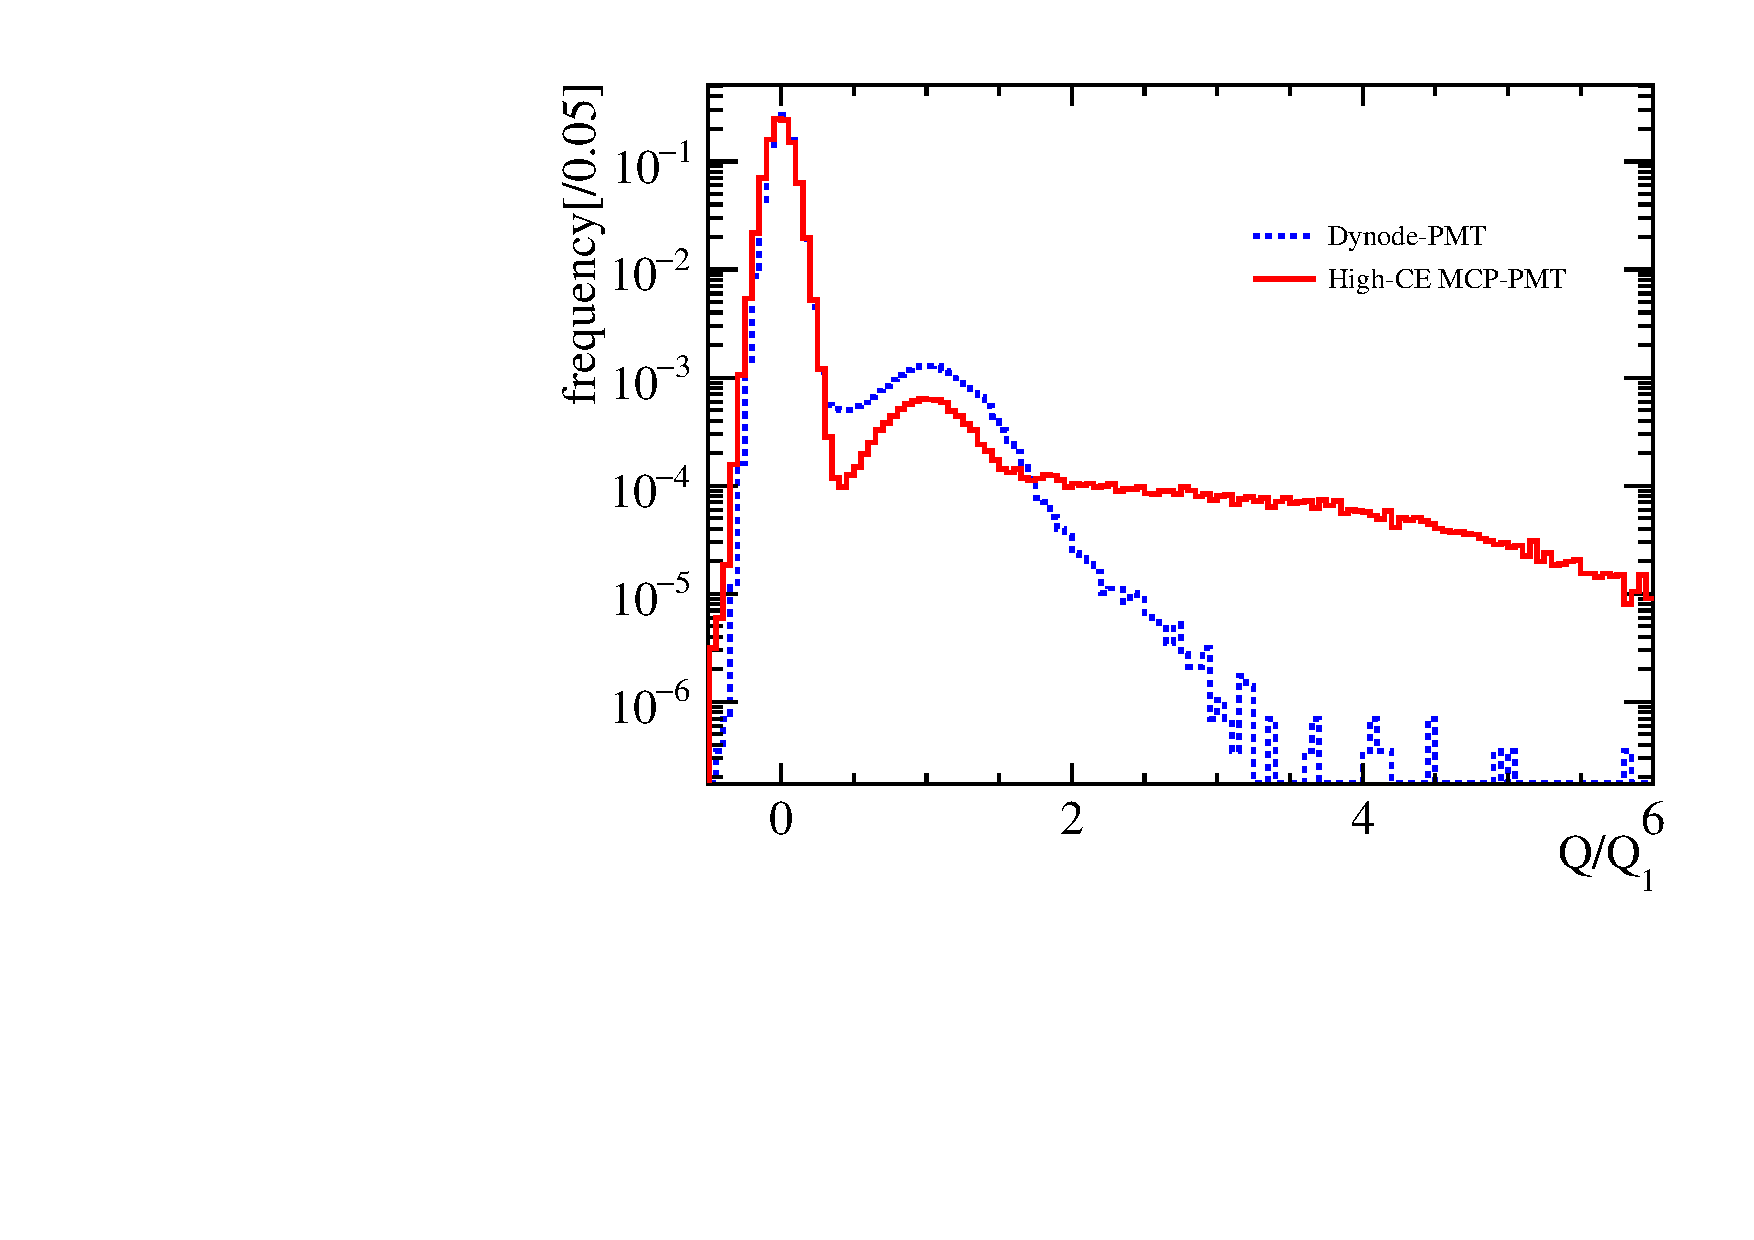
\includegraphics[width=0.9\textwidth]{PMTRelated/GTmodel/spe.pdf}
	\caption{The charge spectrum of the high-CE MCP-PMT GDB-6082~(red) and a dynode-PMT~(blue)~\cite{Zhang:2023ued}.
		The blue histogram consists of the pedestal $Q=0$ and the principal peak of $Q=Q_1$, while the red histogram includes jumbo charges.}
	\label{fig:spe_sreal}
\end{figure}

\subsection{Gamma-Distributed SER charges}\label{gammapossion}
Electron multiplication at dynodes or MCP channels follows an approximately Poisson-distributed process~\cite{branchandPoisson}. Successive multiplications constitute a cascaded Poisson sequence~\cite{1955Scintillation}, representing a branching process~\cite{Bartlett1963TheTO} that poses significant challenges for analytical computation. Woodward~\cite{Woodward} observed that the SER charge spectrum exhibits an intermediate morphology between Poissonian and Gaussian distributions. To characterize electron multiplication in PMTs, particularly accounting for dynode surface non-uniformity, Prescott~\cite{polya} proposed a cascaded Polya distribution. Kalousis~\cite{2012Calibration,2020A} subsequently approximated the Polya distribution as a Gamma form for PMT calibration, demonstrating enhanced performance compared to the Gaussian model in Eq.~\eqref{eq:sreal}.

We adopt a Gamma distribution $\varGamma(\alpha, \beta)$ parametrized by scale factor $\alpha$ and rate factor $\beta$ (Eq.~\eqref{eq:gamma}), thereby eliminating the nonphysical sub-zero tail inherent in Gaussian representations.
\begin{equation}
	\label{eq:gamma}
	\begin{aligned}
		f_\Gamma(x ; \alpha, \beta) = \frac{x^{\alpha-1} e^{-\beta x} \beta^\alpha}{\Gamma(\alpha)} \quad \text { for } x>0 \quad \alpha, \beta>0 \\
	\end{aligned}
\end{equation}
where $\Gamma(\alpha)$ is the Gamma function.
A Gamma distribution is uniquely determined by its expectation value \(\alpha/\beta=Q_1\) and variance \(\alpha/\beta^2=\sigma_1^2\),
which can be converted into the Gaussian counterparts in Eq.~\eqref{eq:sreal}.
The charge spectrum based on the Gamma distribution is,
\begin{equation}
	\begin{aligned}
		f(Q) & = & P_{\pi}(n_{\mathrm{PE}}=0;\lambda)f_{\mathrm{b}}(Q) + \sum_{n_{\mathrm{PE}}=1}^{\infty}P_\pi(n_{\mathrm{PE}};\lambda) f_\Gamma(Q;n_{\mathrm{PE}}\alpha, \beta). \\
	\end{aligned}
	\label{eq:Gamma}
\end{equation}

\subsection{Jumbo Charges through Extra Multiplication}\label{sec:see}
SEE has garnered significant research interest due to its critical role in vacuum electronic devices. Bruining's seminal monograph \textit{Physics and Applications of Secondary Electron Emmision}~\cite{bruining_physics_1954} consolidated foundational methodologies, empirical findings, and technological implementations of SEE. Baroody~\cite{baroody1950theory} proposed a metallic SEE theory postulating that incident primary electrons interact exclusively with conduction-band free electrons, neglecting energy-dependent variations in secondary emission. Dekker~et~al.~\cite{dekker1952theory} established a quantum theory addressing Coulomb interactions between incident primaries and lattice electrons. Wolff~\cite{wolff1954theory} developed the cascade theory describing secondary electron diffusion, energy dissipation, and multiplication within metals.

Under isotropic conditions for incident and backscattered electrons, Kanaya~et~al.~\cite{Kanaya_1978} derived SEY values for insulators incorporating ionization potentials, valence electron contributions, backscattering coefficients, and free-electron density effects. Vaughan~\cite{vaughan} empirically expressed SEY as a function of impact energy and direction~(the Vaughan model), enabling computational implementation. Furman and Pivi~\cite{2002Probabilistic} created a mathematically self-consistent Monte Carlo framework~(the Furman model) characterizing SEE from solid surfaces. This model probabilistically describes secondary emission statistics, treating emitted electron energies as independent, identically distributed random variables governed by material properties and primary energies.

Whereas early theoretical models emphasized mechanistic explanations, the Vaughan and Furman frameworks prioritize Monte Carlo computational methods. The Furman model achieves superior physical consistency and experimental agreement, justifying its selection for precision applications requiring adaptable parameters and enhanced accuracy.

\subsubsection{Furman probabilistic model}\label{subsec:fuman}
In the Furman model~\cite{2002Probabilistic}, there are three kinds of secondary electrons, as shown in Fig.~\ref{fig:furmanelectrons}.
\begin{figure}
	\centering
	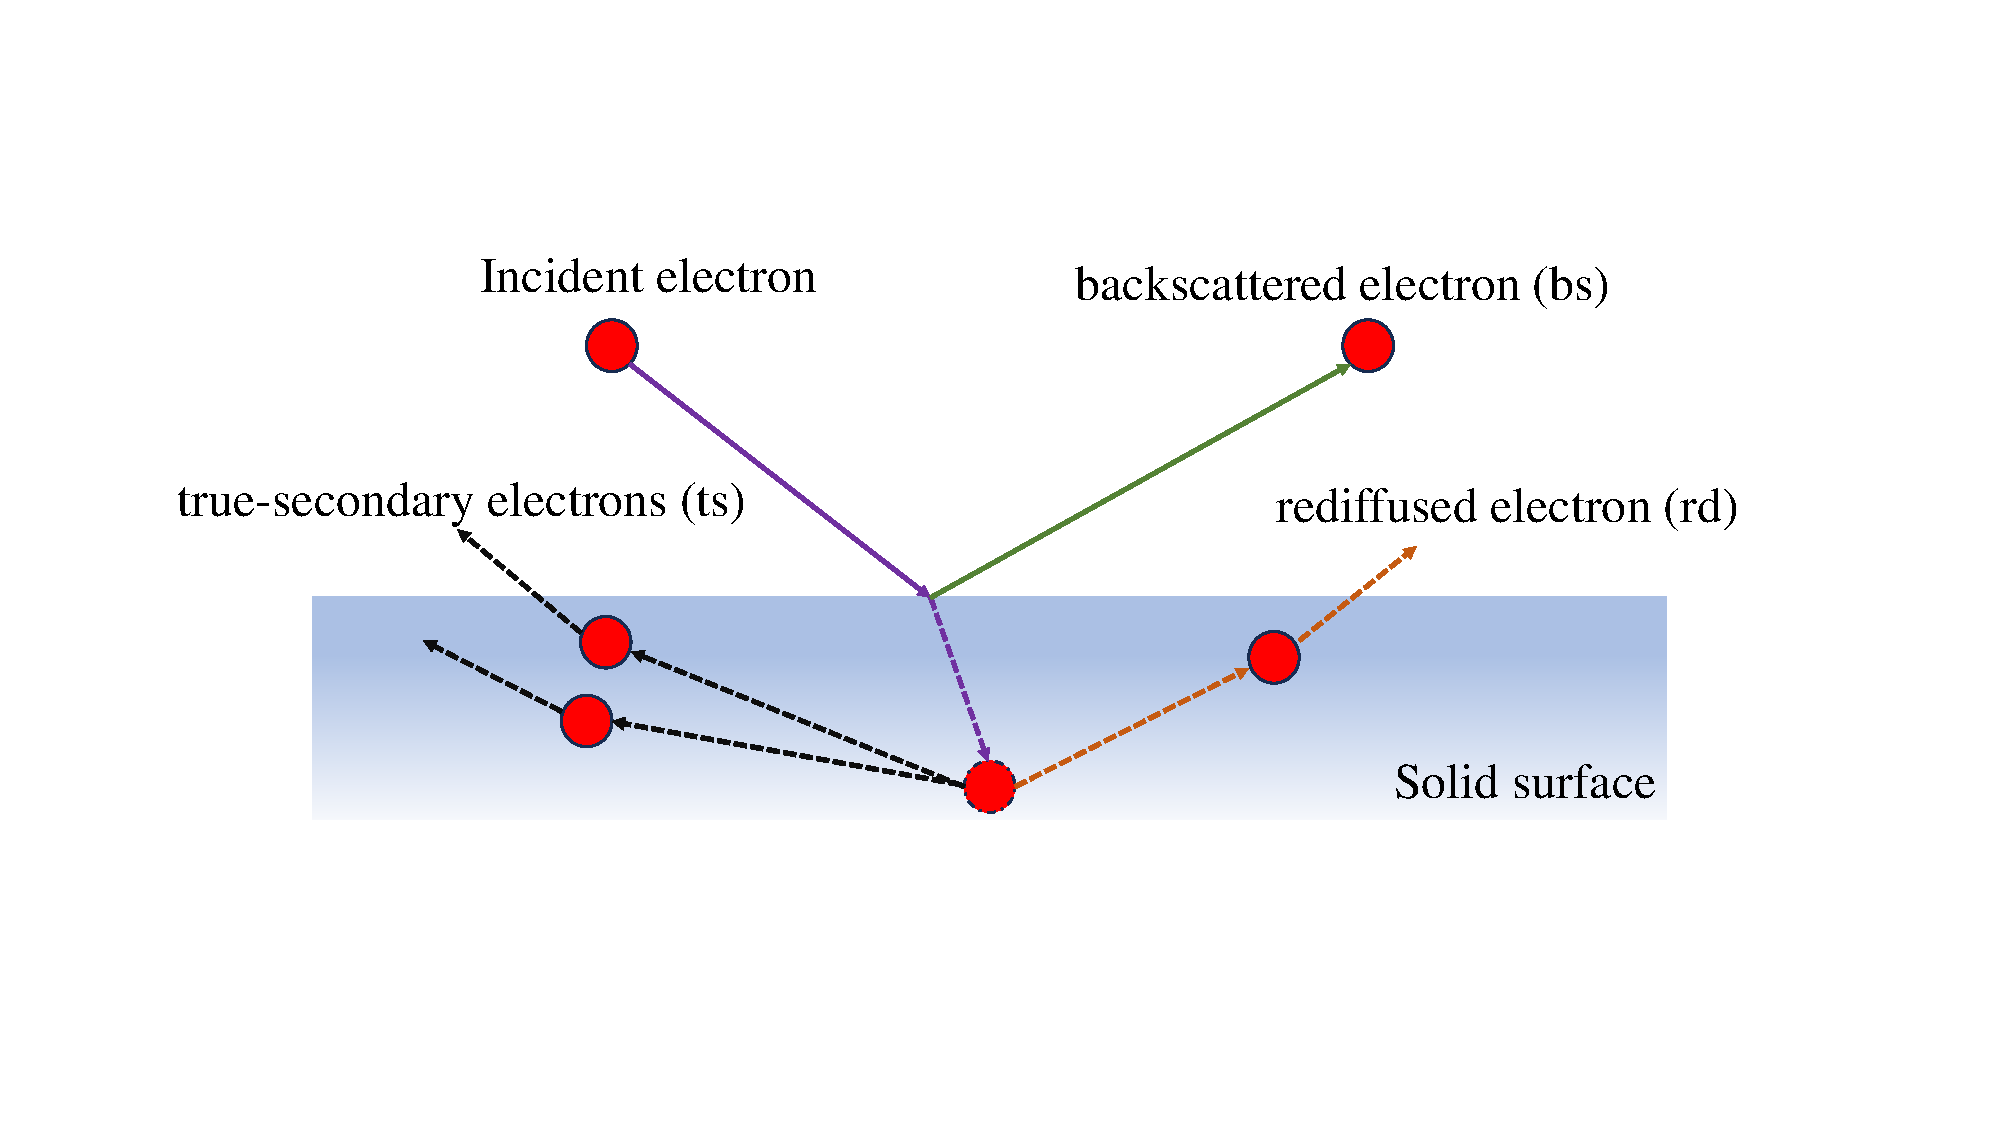
\includegraphics[width=0.9\textwidth]{PMTRelated/GTmodel/furman.pdf}
	\caption{The three kinds of secondary electrons in Furman model.}
	\label{fig:furmanelectrons}
\end{figure}
The first type is the backscattered electrons emitted through elastic scattering on the surface of the target material. Its energy distribution $\mathrm{d}\delta_{\mathrm{bs}}/\mathrm{d}E$ is given by Eq.~\eqref{eq:backscatter}, where $\delta_{\mathrm{bs}}$ represents the yield of backscattered electrons, the Heaviside function $\theta(E)$ ensures that $E < E_0$, $E_0$ is the energy of the incident primary electrons, $\theta_0$ is the incident angle, and $\sigma_{\mathrm{bs}}$ is the adjustable standard deviation.
\begin{equation}
	\label{eq:backscatter}
	\begin{aligned}
		 & \frac{\mathrm{d}\delta_{\mathrm{bs}}}{\mathrm{d}E} =\theta(E) \theta\left(E_0-E\right) \delta_{\mathrm{bs}}\left(E_0, \theta_0\right)
		\frac{2 \exp \left(-\left(E-E_0\right)^2 / 2 \sigma_{\mathrm{bs}}^2\right)}{\sqrt{2 \pi} \sigma_{\mathrm{bs}}
		\operatorname{erf}\left(E_0 / \sqrt{2} \sigma_{\mathrm{bs}}\right)}                                                                      \\
	\end{aligned}
\end{equation}

After penetrating the target material, some electrons are inelastically scattered by atoms and reflected out, forming the second type of electrons. Leonard referred to the bending of the electron trajectory as ``diffusion``, and in German literature, a $90^\circ$ turn of the trajectory is called \text {``Rückdiffusion''} in German literature~\cite{bruining_physics_1954}. Furman and Pivi~\cite{2002Probabilistic} adopted this convention and named them \emph{rediffused electrons}. The energy distribution of rediffused electrons is defined by Eq.~\eqref{eq:rediffused}, where $\delta_{\mathrm{rd}}$ is the yield of rediffused electrons and $q$ is an adjustable parameter.

\begin{equation}
	\label{eq:rediffused}
	\begin{aligned}
		 & \frac{\mathrm{d}\delta_{\mathrm{rd}}}{\mathrm{d}E} =\theta(E) \theta\left(E_0-E\right) \delta_{\mathrm{rd}}\left(E_0, \theta_0\right) \frac{(q+1) E^q}{E_0^{q+1}} \\
	\end{aligned}
\end{equation}

The last but the most important kind is the true-secondary electrons.
Upon deeper penetration of electrons into the target material, intricate physical processes ensue,
generating one or more secondaries.
This is the process of multiplying electrons.
The spectrum is defined as Eq.~\eqref{eq:true}.
\begin{equation}
	\label{eq:true}
	\begin{aligned}
		\frac{\mathrm{d} \delta_{\mathrm{ts}}}{\mathrm{d} E} =  \sum_{n=1}^{\infty}
		 & \frac{n P_{n,\mathrm{ts}}\left(n; \delta_{\mathrm{ts}}(E_0,\theta_0)\right)
		\left(E / \epsilon_{n}\right)^{p_{n}-1} e^{-E / \epsilon_{n}}}
		{\epsilon_{n} \Gamma\left(p_{n}\right) \Upsilon\left(n p_{n}, E_0 / \epsilon_{n}\right)} \\
		 & \times \Upsilon\left[(n-1) p_{n},\left(E_0-E\right) / \epsilon_{n}\right]
	\end{aligned}
\end{equation}
where $\delta_{\mathrm{ts}}(E_0,\theta_0)$
is the yield of the true-secondary electrons when the incident energy is $E_0$ and the incident angle is $\theta_0$,
$\epsilon_{n}>0$ and $p_{n}>0$ are the phenomenological parameters.
$\gamma(z,x)$ is the incomplete gamma function,
and $\Upsilon(z,x)=\gamma(z,x)/\Gamma(z)$ is the normalized form satisfying $\Upsilon(0,x)=1$.
$n$, the number of the true-secondary electrons, follows a Poisson distribution~$\mathrm{\pi}(\delta_{\mathrm{ts}}(E_0,\theta_0))$.
$P_{n,\mathrm{ts}}$ is its probability mass function.

where $\delta_{\mathrm{ts}}(E_0,\theta_0)$ represents the yield of the true-secondary electrons under the conditions that $E_0$ is the incident energy and $\theta_0$ is the incident angle. Here, $\epsilon_{n}>0$ and $p_{n}>0$ work as the phenomenological parameters. $\gamma(z,x)$ is the incomplete gamma function, and its normalized form is $\Upsilon(z,x)=\gamma(z,x)/\Gamma(z)$ satisfying $\Upsilon(0,x)=1$ . The number of the true-secondary electrons $n$ follows the Poisson distribution $\mathrm{\pi}(\delta_{\mathrm{ts}}(E_0,\theta_0))$, and its probability mass function is $P_{n,\mathrm{ts}}$.

As illustrated in Fig.~\ref{fig:SES}, the parameters~\cite{2021Effects} are setted as
$\delta_{\mathrm{bs}}=0.05$, $\delta_{\mathrm{rd}}=0.5$, $\delta_{\mathrm{ts}}=5$,
$\theta_0=0^\circ$ and $E_0=\SI{650}{eV}$.
The total spectrum is the sum of three components.
\begin{equation}
	\frac{\mathrm{d}\delta}{\mathrm{d}E}=\frac{\mathrm{d}\delta_{\mathrm{bs}}}{\mathrm{d}E} + \frac{\mathrm{d}\delta_{\mathrm{rd}}}{\mathrm{d}E} + \frac{\mathrm{d}\delta_{\mathrm{ts}}}{\mathrm{d}E}
\end{equation}

When the incident energy~$E_0$ is around \SI{650}{eV}, the energies of the secondaries are usually less than \SI{100}{eV} .
\begin{figure}[htbp]
	\centering
	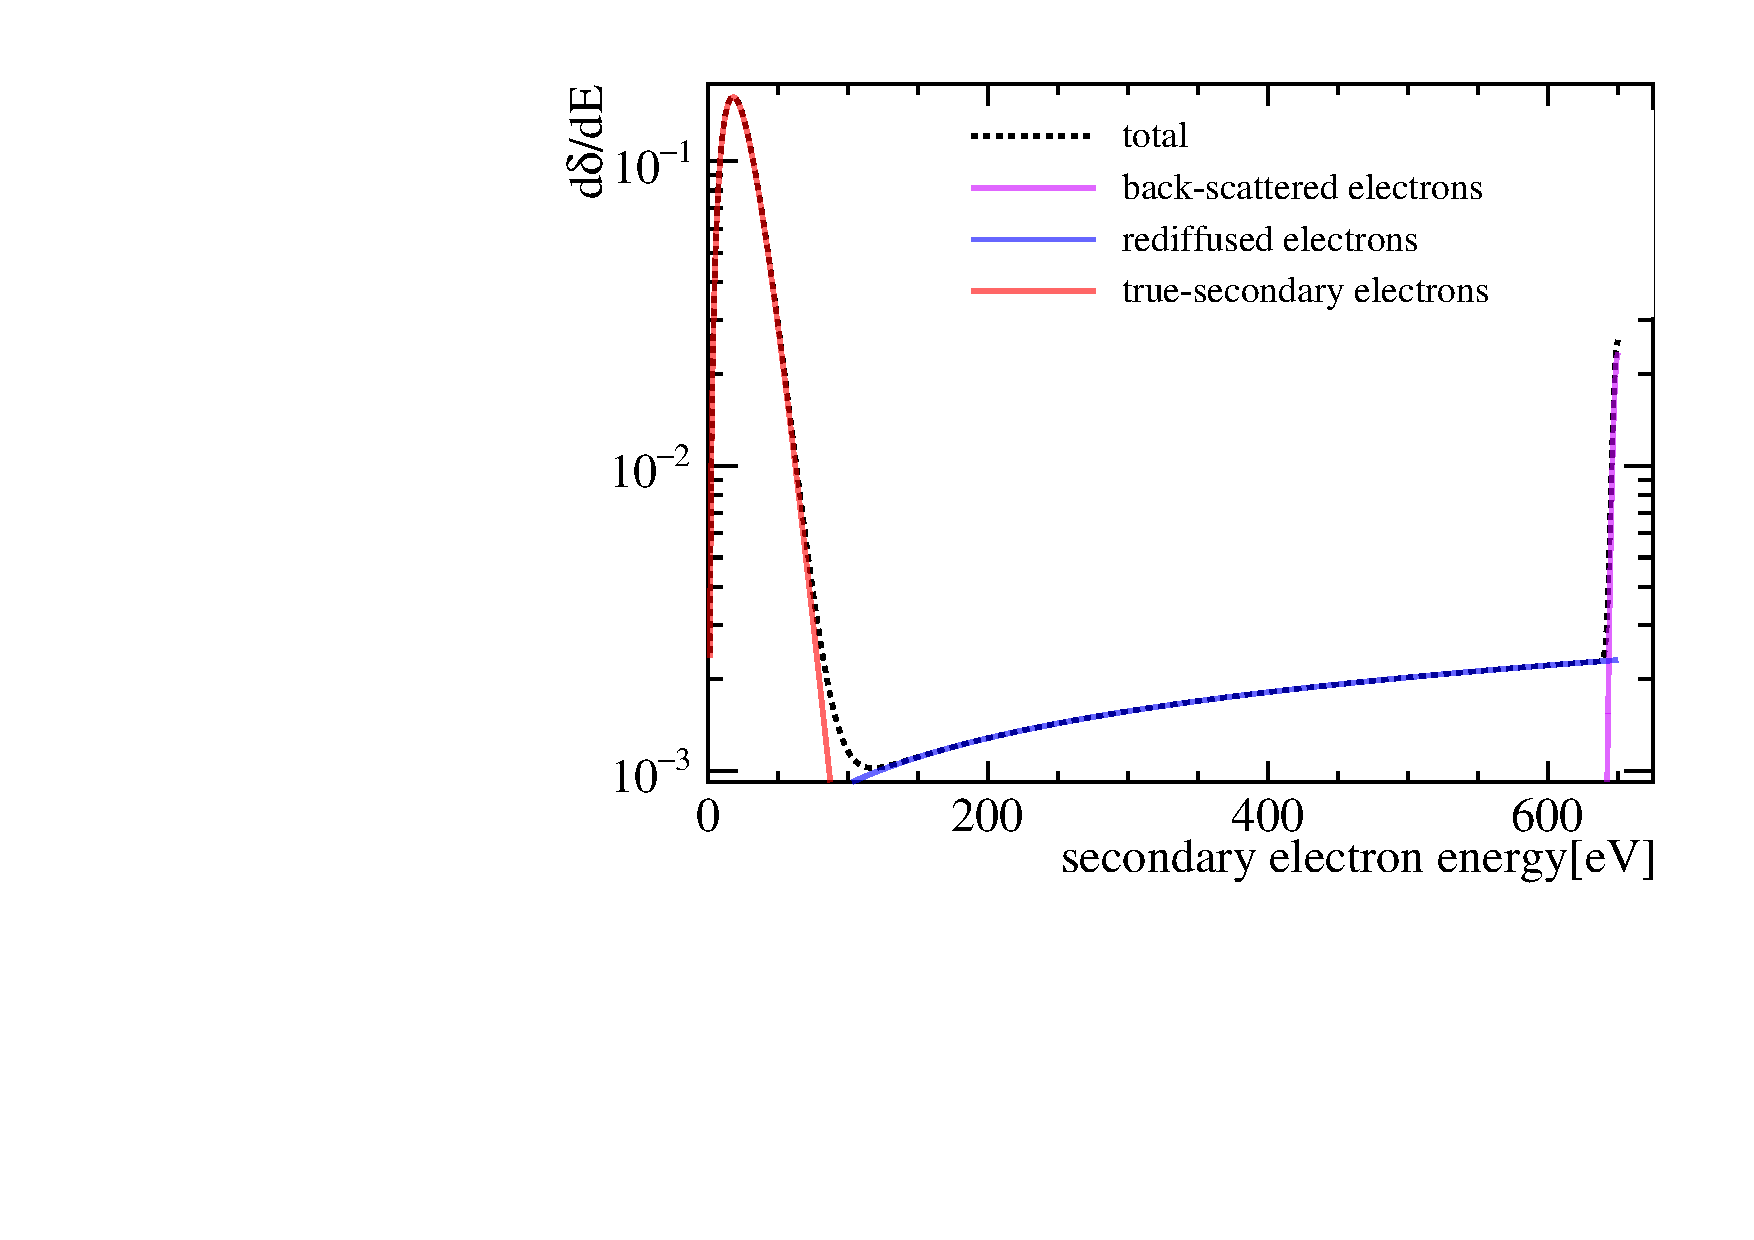
\includegraphics[width=0.7\textwidth]{PMTRelated/GTmodel/SES.pdf}
	\caption{The total energy spectrum of the secondary electrons when the incident energy is \SI{650}{eV}.
		The violet, blue, and red lines represent $\mathrm{d}\delta_{\mathrm{bs}}/\mathrm{d}E$, $\mathrm{d}\delta_{\mathrm{rd}}/\mathrm{d}E$, and
		$\mathrm{d}\delta_{\mathrm{ts}}/\mathrm{d}E$, repectively.
		The black dashed line is $\mathrm{d}\delta/\mathrm{d}E$.}
	\label{fig:SES}
\end{figure}

\subsubsection{An extra multiplication mode}
A Chevron stack of two MCPs as the electron multiplier is used in the MCP-PMT both in JUNO and JNE.
As shown in Fig.~\ref{fig:circuit}, through the ALD technology, an \ce{Al2O3}-\ce{MgO}-\ce{Al2O3} layer~\cite{zzj2021Al} is deposited not only on the channel surface of the lead glass body
but also on the entrance electrode M1 of the first MCP.

Such a design enables each PE to have two potential amplification methods, as shown in Fig.~\ref{fig:circuit}.
In the channel mode, they directly penetrate the channels; in the surface mode, they strike $\mathrm{M}1$, generating secondary electrons that subsequently enter the channels, as detailed in ~\cite{2016Optimization}. Once inside the MCP channel, the electrons undergo multiple collisions with the channel wall, leading to amplification through a series of multiplicative processes, as described in~\cite{1955Scintillation}

The choice of these two routes constitutes a Bernoulli trial~\cite{1955Scintillation}. Regarding those low-energy secondary electrons in the surface mode, the MCP gain is significantly lower than that of the primary PEs in the channel mode, as reported in Ref.~\cite{2012An}.

\subsubsection{Voltage-division Experiment}\label{sec:gain}
The dependence of the MCP gain for an electron versus its incident energy at the
channel entrance is crucial to understanding the jumbo charges.
We designed a voltage-division experiment to measure such a relationship.
It is of critical importance for the origin of the jumbo charges to understand the dependence of the MCP gain for an electron on its incident energy at the channel entrance. To measure such a relationship, we devised a voltage-division experiment.

As shown in Fig~\ref{fig:circuit},  a positive high-voltage power supply~(positive HV) was utilized to keep the potentials applied
to the MCPs stable through the circuit~\cite{Luo:2023jdf}.  In parallel, a negative high-voltage power supply~(negative HV) was taken to vary the electric
potential difference between the photocathode and $\mathrm{M}1$, which can help get PEs at different incident energies.
Our circuit design was adapted from the circuit implementation presented in~\cite{Luo:2023jdf}. In our modification, we eliminated the redundant resistors R1 and R2, while keeping the remaining resistors unaltered.
In comparison with the experiment conducted by Yang et al. \cite{2017MCP}, in which the potentials of all electrodes M1 - 4 are controllable, our design represents a simplified adaptation. This adaptation is specifically aimed at tuning the energies of the PEs using commercially available HV products.

\begin{figure}[!ht]
	\centering
	\includegraphics[width=\textwidth]{PMTRelated/GTmodel/set.pdf}
	\caption{
		In the context of MCP operation, $\mathrm{M}1$ and $\mathrm{M}3$ serve as the input electrodes, while $\mathrm{M}2$ and $\mathrm{M}4$ function as the output electrodes. These four electrodes establish the potential differences essential for the device's operation. }
	\label{fig:circuit}
\end{figure}

A picosecond laser with a wavelength of \SI{405}{nm} was used to illuminate the MCP-PMT at \SI{1}{kHz} rate. The laser also feed an electronic trigger signal to capture waveform data.
We adjusted the intensity of the picosecond laser until the occupancy was below 0.1 to obtain the single PE.

A 10-bit oscilloscope~(HDO9000 with HD1024 Technology)~\cite{teledynelecroy} was utilized to capture the \SI{100}{ns} waveform. This oscilloscope worked at a sampling rate of \SI{40}{GS/s} and a range of [-20, 60]~\si{mV}.

We obtained the MCP gain at different incident energies of the electrons by fitting the Gaussian on the charge distribution. To control the experimental variables and contrast the effect of the surface mode, the same experiment were conducted on two MCP-PMTs with~(Fig.~\ref{fig:gain_ald}) and without~(Fig.~\ref{fig:gain_noald}) \ce{Al2O3}-\ce{MgO} deposited on $\mathrm{M}1$.
The positive voltage for the MCP-PMT with \ce{Al2O3}-\ce{MgO} on M1 was +\SI{1205}{V} after calculation and for that without \ce{Al2O3}-\ce{MgO} on M1 was +\SI{1240}{V}, respectively.
The energies of the PEs when generated at the photocathod are \SI{\sim 1}{eV}~\cite{Nathan1970TheED} and the error of the negative HV itself is within \SI{2}{V}.
The incident energies~($E_0$) can be treated as the energies that the PEs get in the electric field, numerically equal to the voltage between the photocathode and M1, with a systematic error of $\pm$\SI{2}{eV}.
The MCP gain was scanned every \SI{10}{eV} when $10\leqslant E_0<100$~\si{eV}, every \SI{20}{eV} when $100\leqslant E_0<200$~\si{eV}
and every \SI{50}{eV} when $200<E_0\leqslant 650$~\si{eV}.
The scan range is $10\leqslant E_0\leqslant 600$~\si{eV} for the MCP-PMT with \ce{Al2O3}-\ce{MgO} deposited on M1 and $10\leqslant E_0\leqslant 680$~\si{eV} for that without.

The charges of the captured waveforms were measured using \emph{fast stochastic matching pursuit} (FSMP)~\cite{Xu_2022,Wang_2024}. This method can suppress the interference of electronic noise, enabling the acquisition of accurate charge spectra across a wide range of gain. Due to FSMP's capacity to PEs, the charge is zero when $n_{\mathrm{PE}} = 0$, and the pedestal is clearly removed from the charge distribution.
In Fig.~\ref{fig:gain_fit}, the peaks are associated with the channel mode. The jumbo charges coming from the surface mode are located to the right of the peaks, while the insufficient amplifications are to the left. For the MCP-PMT without \ce{Al2O3}-\ce{MgO} deposited on $\mathrm{M}1$, since the contribution of secondaries from the surface mode is minimal, there are no large charges in the charge spectrum, as depicted in Fig.~\ref{fig:gain_noald}. To determine the MCP gain for electrons in channel mode, only the peak was fitted to eliminate the influence of the surface mode.

We acquired approximate values of $\mu_{\mathrm{p}}$ and $\sigma_{\mathrm{p}}$ for the charge distribution. These values were used to supply initial values and ranges for a detailed fitting process. The fitting ranges were decided based on the incident energies of the PEs. Specifically, when $E_0>100$~\si{eV}, the range was set as $[\mu_{\mathrm{p}} - 1.3\sigma_{\mathrm{p}}, \mu_{\mathrm{p}}+1.6\sigma_{\mathrm{p}}]$; when $30<E_0\leqslant 100$~\si{eV}, it was $[\mu_{\mathrm{p}} - 0.8\sigma_{\mathrm{p}}, \mu_{\mathrm{p}}+1.6\sigma_{\mathrm{p}}]$; and when $E_0\leqslant 30$~\si{eV}, the range became $[\mu_{\mathrm{p}} - 1.5\sigma_{\mathrm{p}}, \mu_{\mathrm{p}}+1.8\sigma_{\mathrm{p}}]$. To measure the MCP gain for electrons at various energies, it suffices to extract the mean charge $\mu(E_0)$ and the standard deviation $\sigma(E_0)$ of the channel - mode peak.

\begin{figure}[!ht]
	\centering
	\begin{subfigure}[b]{0.5\textwidth}
		\centering
		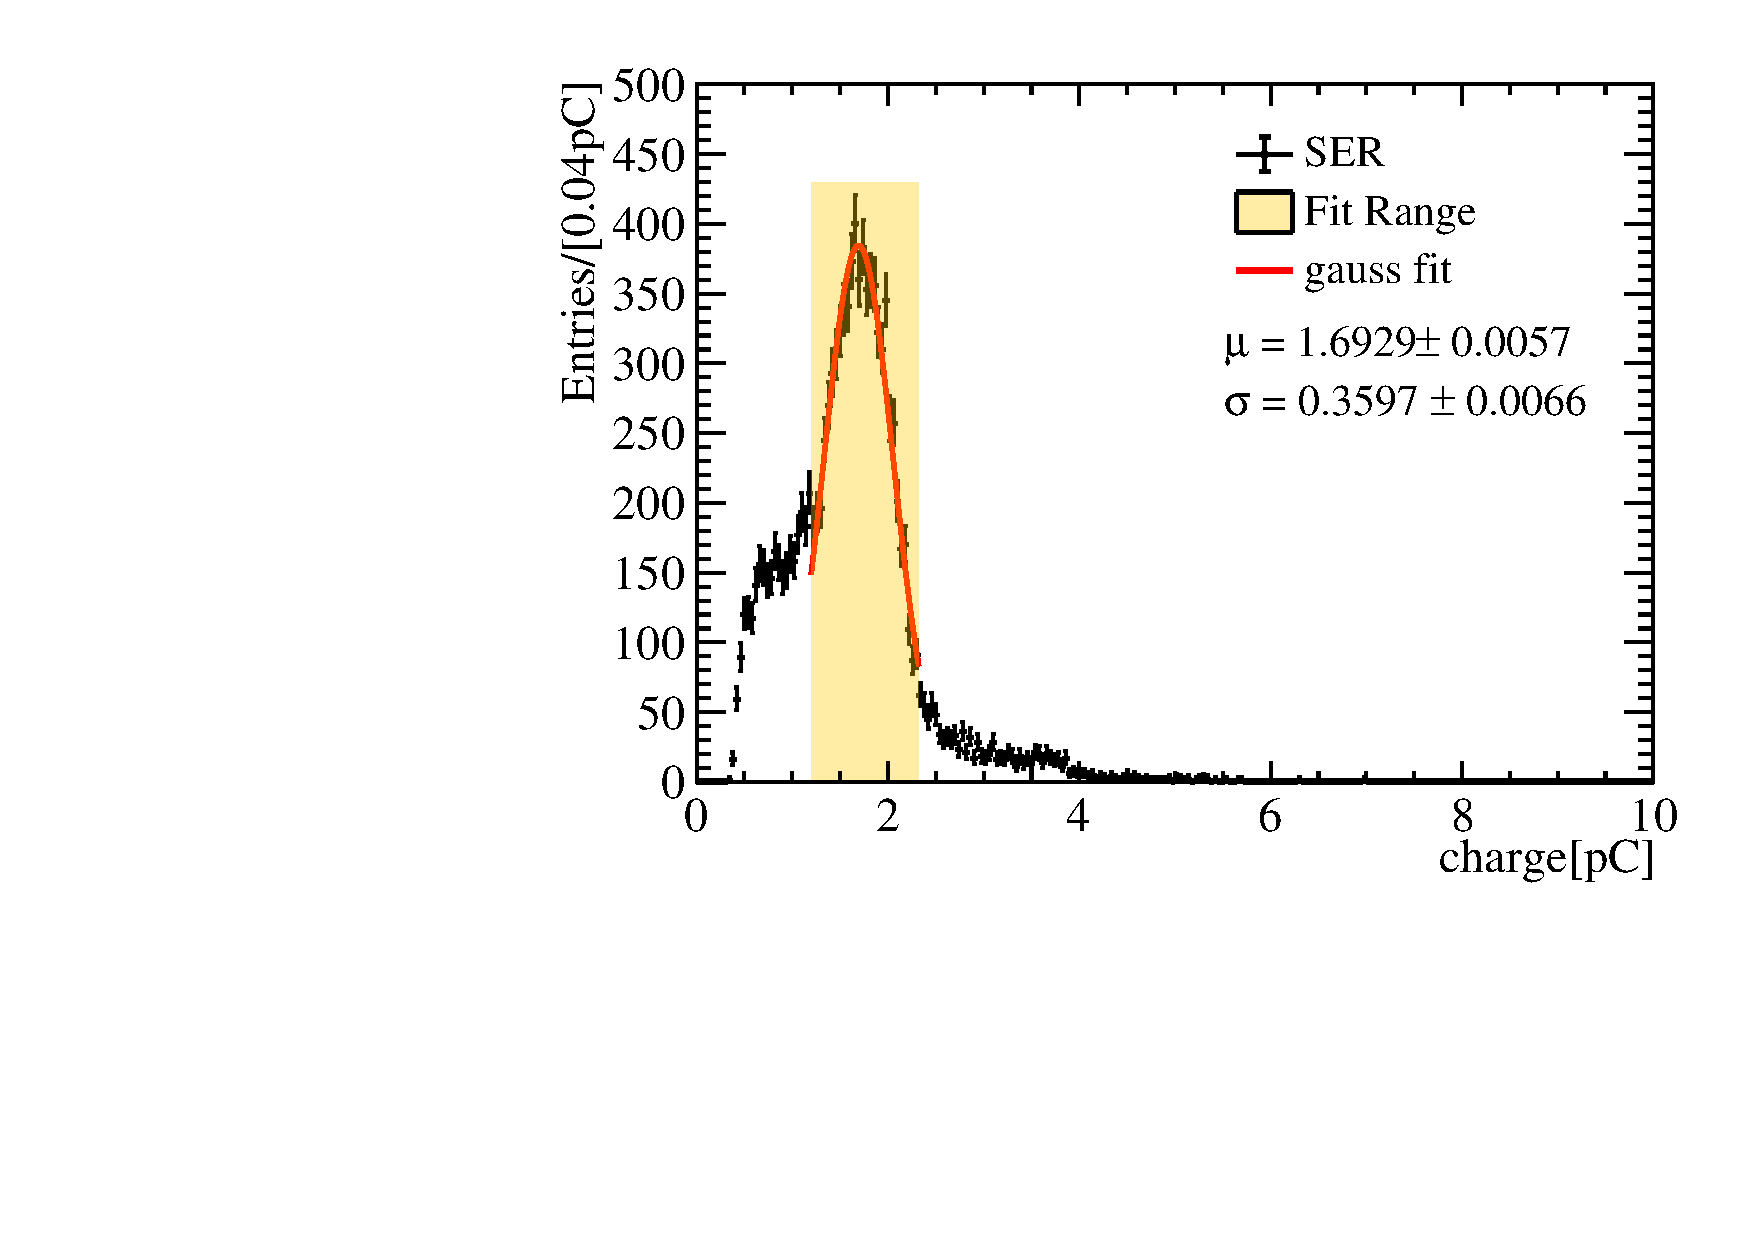
\includegraphics[width=0.9\textwidth]{PMTRelated/GTmodel/fit_noald.pdf}
		\caption{}
		\label{fig:gain_noald}
	\end{subfigure}%
	\hfill
	\begin{subfigure}[b]{0.5\textwidth}
		\centering
		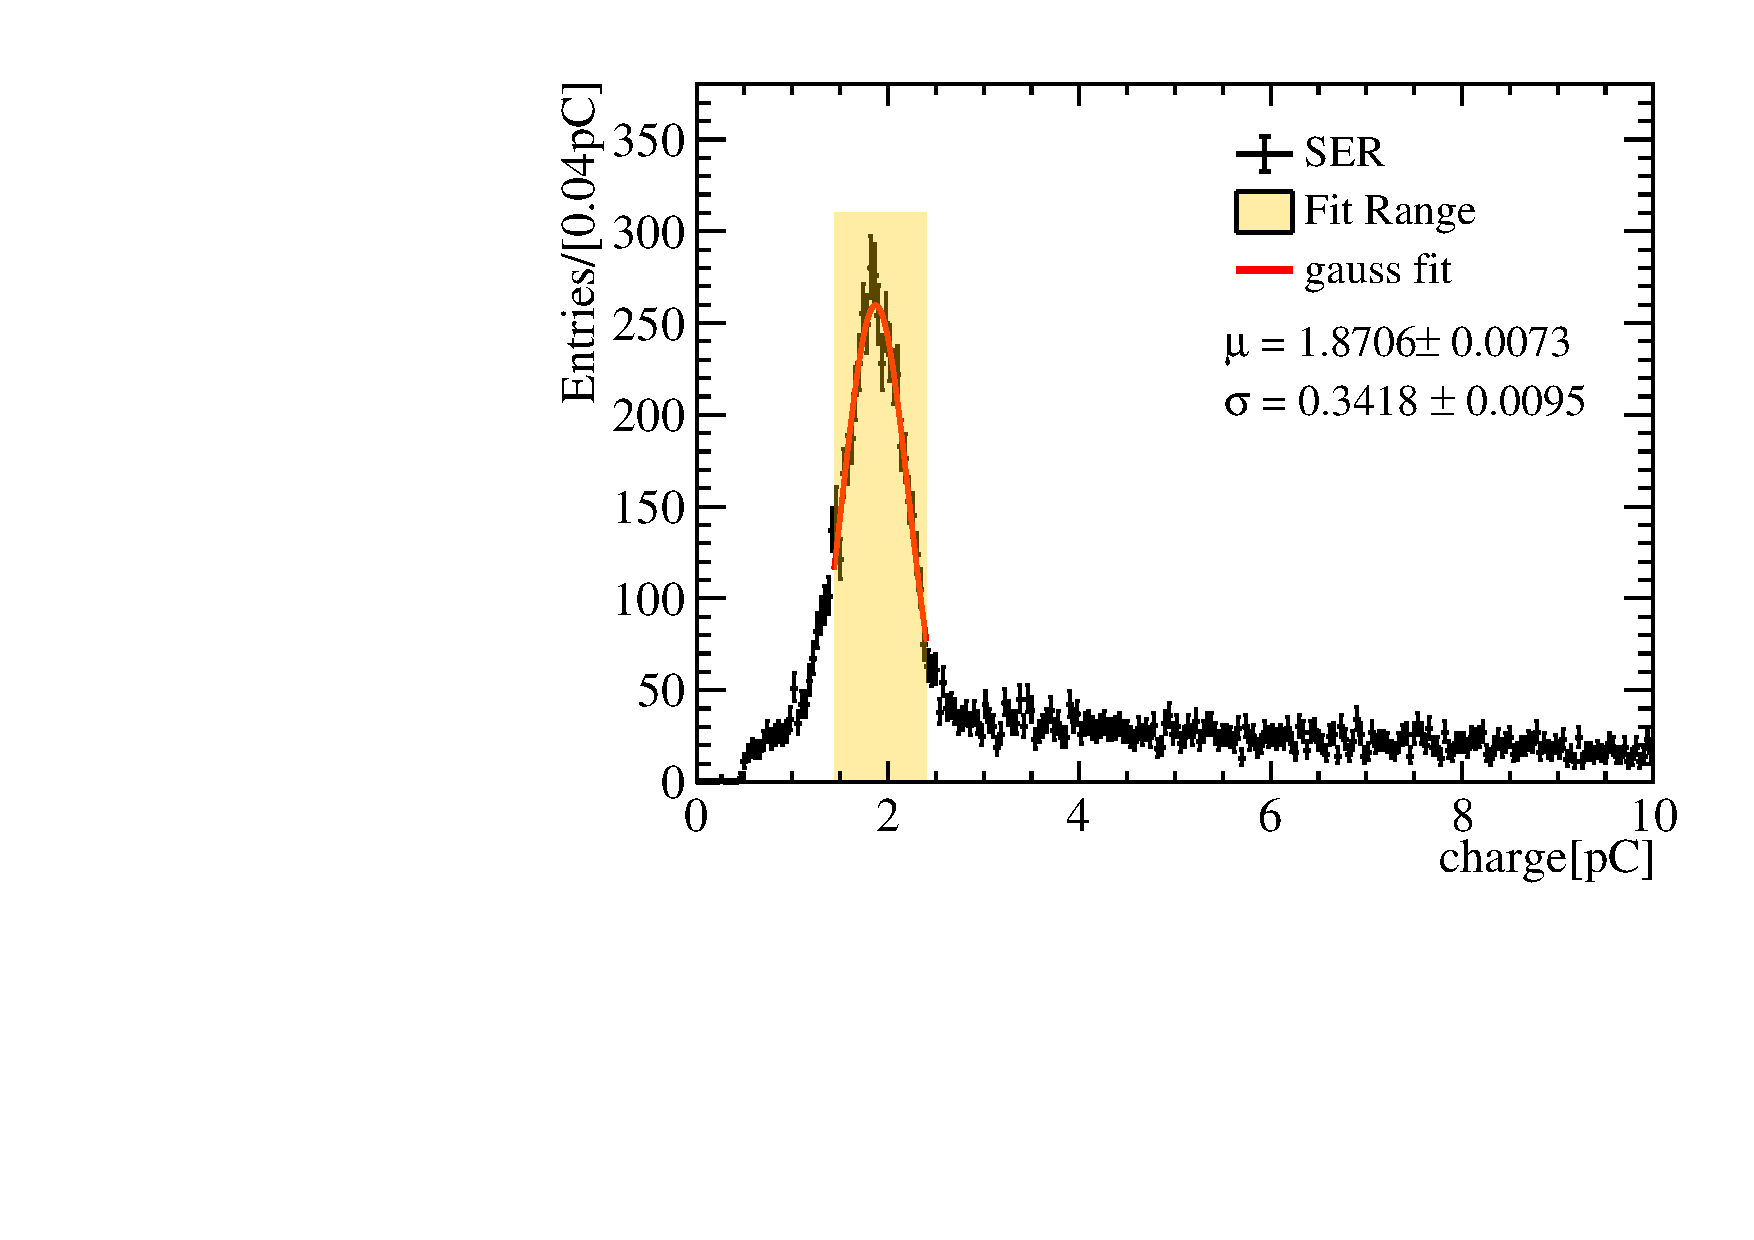
\includegraphics[width=0.9\textwidth]{PMTRelated/GTmodel/fit_ald.pdf}
		\caption{}
		\label{fig:gain_ald}
	\end{subfigure}

	\caption{The fit of the charge spectrum of the MCP-PMT is presented both without \subref{fig:gain_noald} and with \subref{fig:gain_ald} \ce{Al2O3}-\ce{MgO} deposited on $\mathrm{M}1$. It was noticed that \subref{fig:gain_noald} does not show jumbo charges. The yellow regions represent intervals that depend on the incident energy, and the red lines are the fitting outcomes of the Gaussian functions within these intervals.
	}
	\label{fig:gain_fit}
\end{figure}

After performing Gaussian fitting, we conduct linear interpolation and extrapolation to acquire the relationships of $\mu(E_0)$ and $\sigma(E_0)$ presented in Fig.~\ref{fig:gaintest}. The disparity in the relationships of MCP-PMTs with and without \ce{Al2O3}-\ce{MgO} deposited on $\mathrm{M}1$ stems from the impact of the charge contributed by the surface mode. When \(E_0 < \SI{200}{eV}\), $\mu(E_0)$ experiences a rapid increase. Once \(E_0 > \SI{200}{eV}\), $\mu(E_0)$ gradually reaches a stable state. The $\sigma(E_0)$ generally increases in a manner similar to $\mu(E_0)$, yet it shows a decrease around \SI{200}{eV}. Yang et al.~\cite{2017MCP} reported a similar tendency for $\mu(E_0)$. In our study, the optimal relative resolution $\sigma/\mu$ occurs at approximately \SI{600}{eV}, while the results of Yang et al. indicated \SI{200}{eV}. Cao et al.\cite{cao_secondary_2021} discovered that the SEY of \ce{Al2O3}-\ce{MgO} rises with the incident energy within the range of 100 - \SI{600}{eV}. Even though the film structure and thickness we employed are different, taking into account the variation curves of the SEY of \ce{Al2O3} and \ce{MgO} with energy, we can still make a rough evaluation that the trend of $\sigma/\mu$ obtained herein is reasonable.
\begin{figure}[!ht]
	\centering
	\begin{subfigure}[b]{0.5\textwidth}
		\centering
		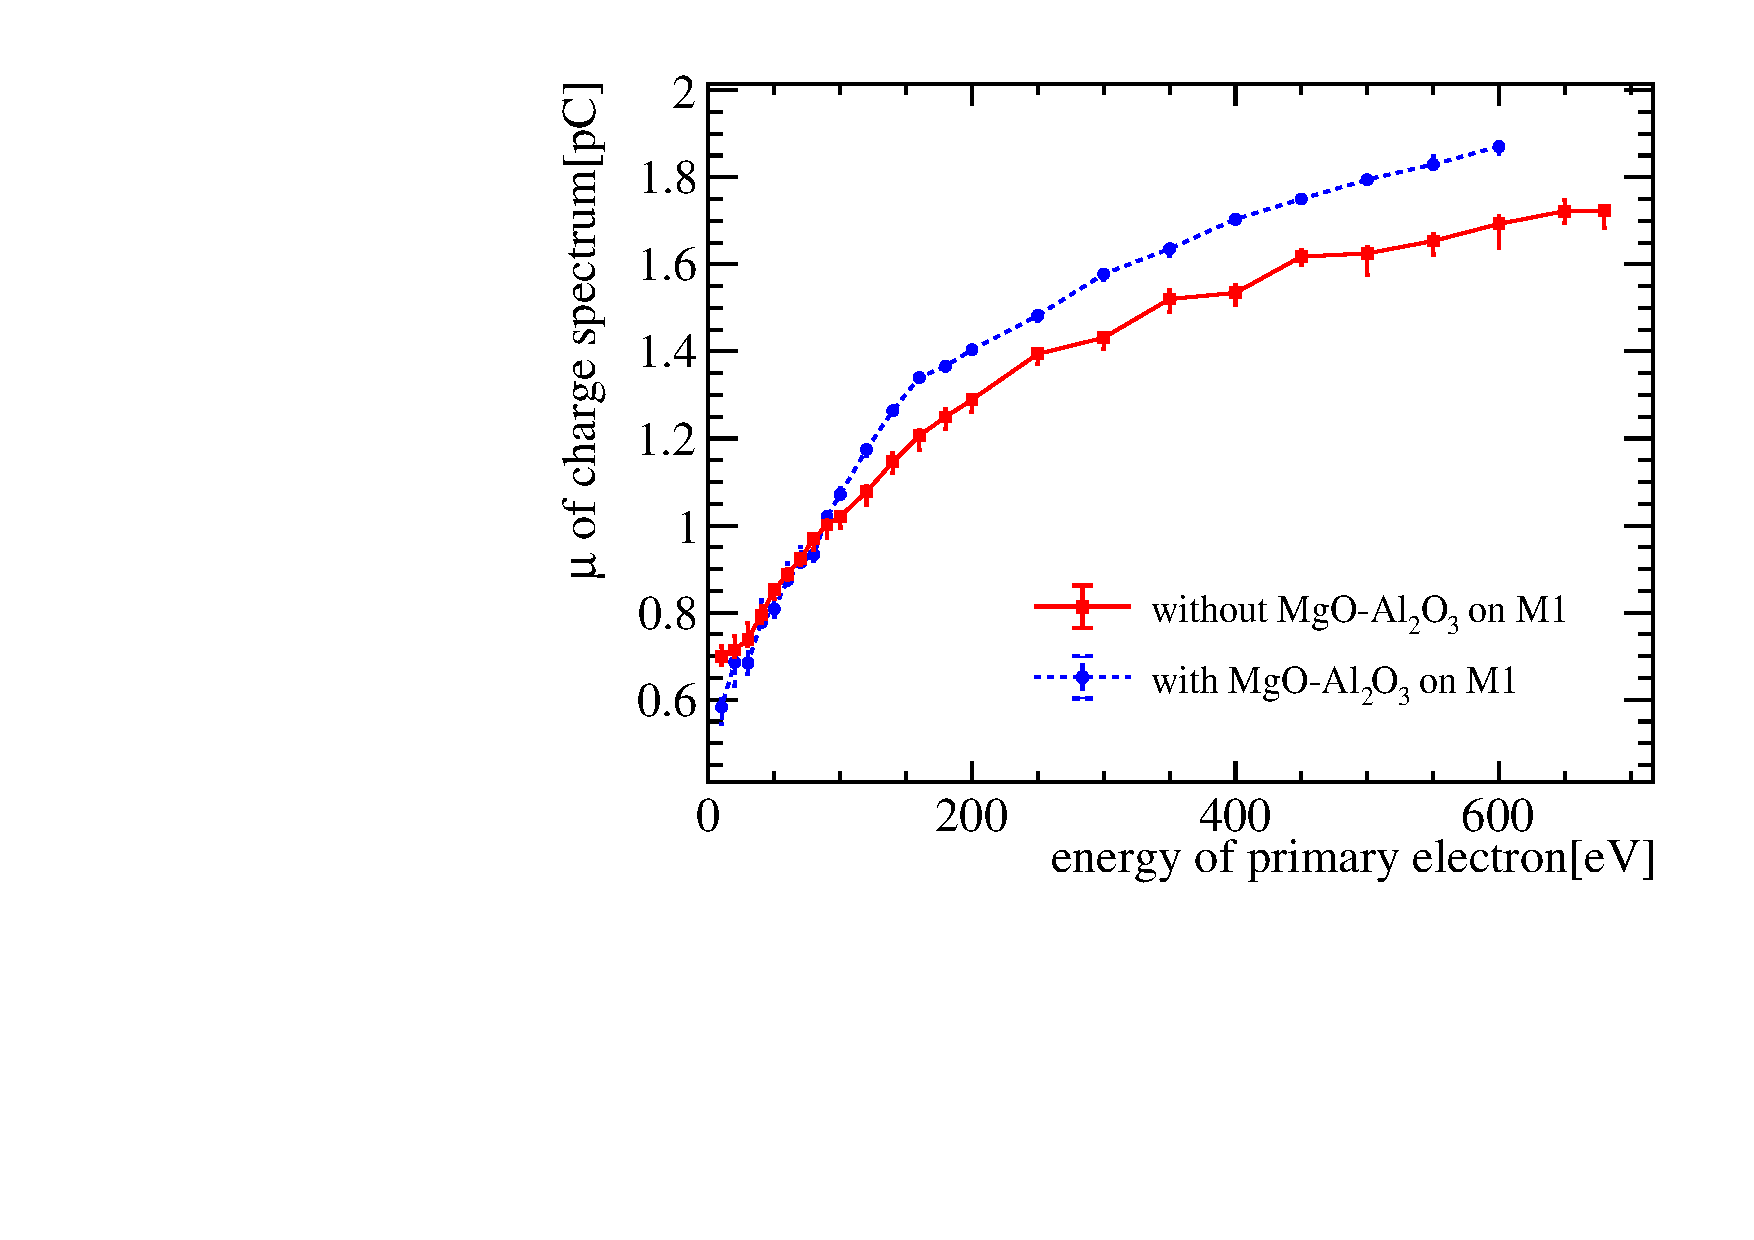
\includegraphics[width=0.9\textwidth]{PMTRelated/GTmodel/gain_mu.pdf}
		\caption{}
		\label{fig:gain}
	\end{subfigure}%
	\begin{subfigure}[b]{0.5\textwidth}
		\centering
		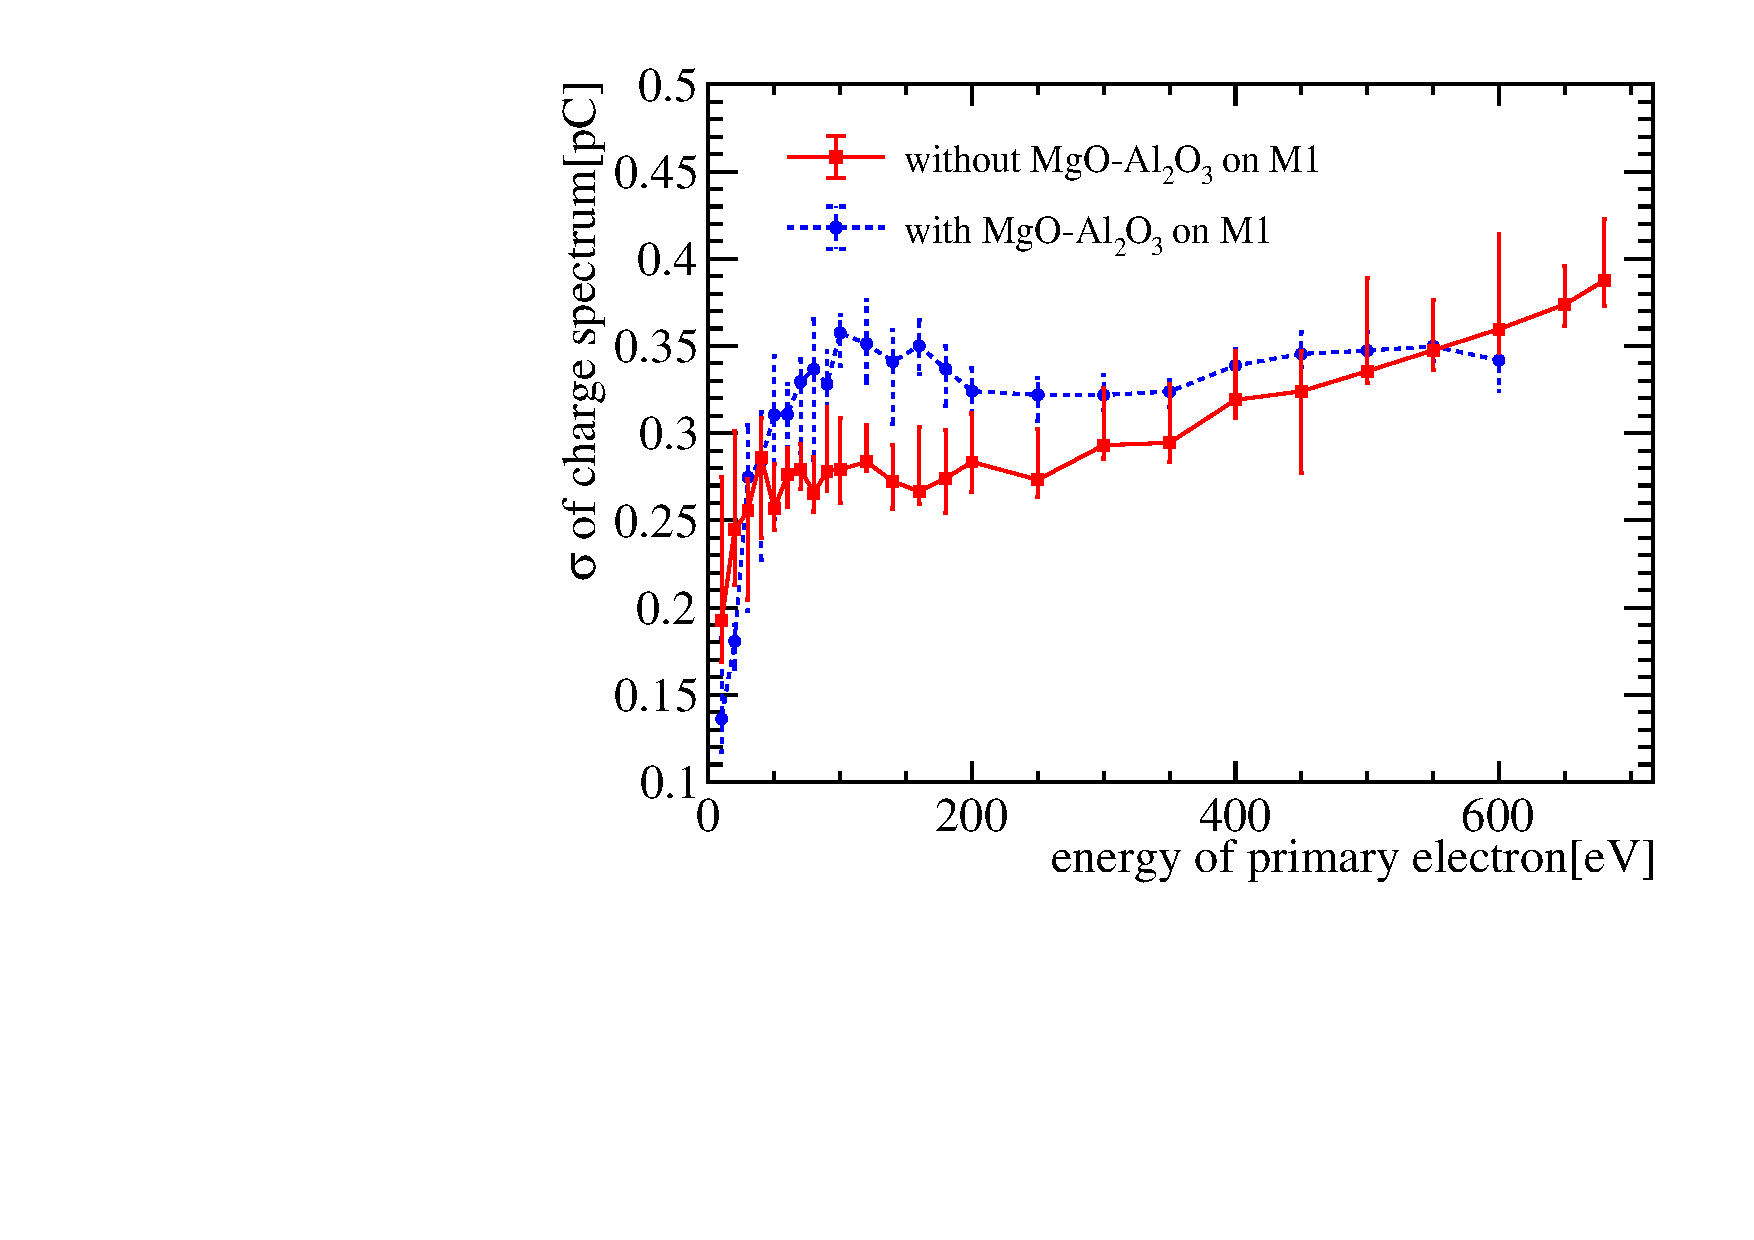
\includegraphics[width=0.9\textwidth]{PMTRelated/GTmodel/gain_sigma.pdf}
		\caption{}
		\label{fig:sigma}
	\end{subfigure}
	\hfill
	\begin{subfigure}[b]{0.5\textwidth}
		\centering
		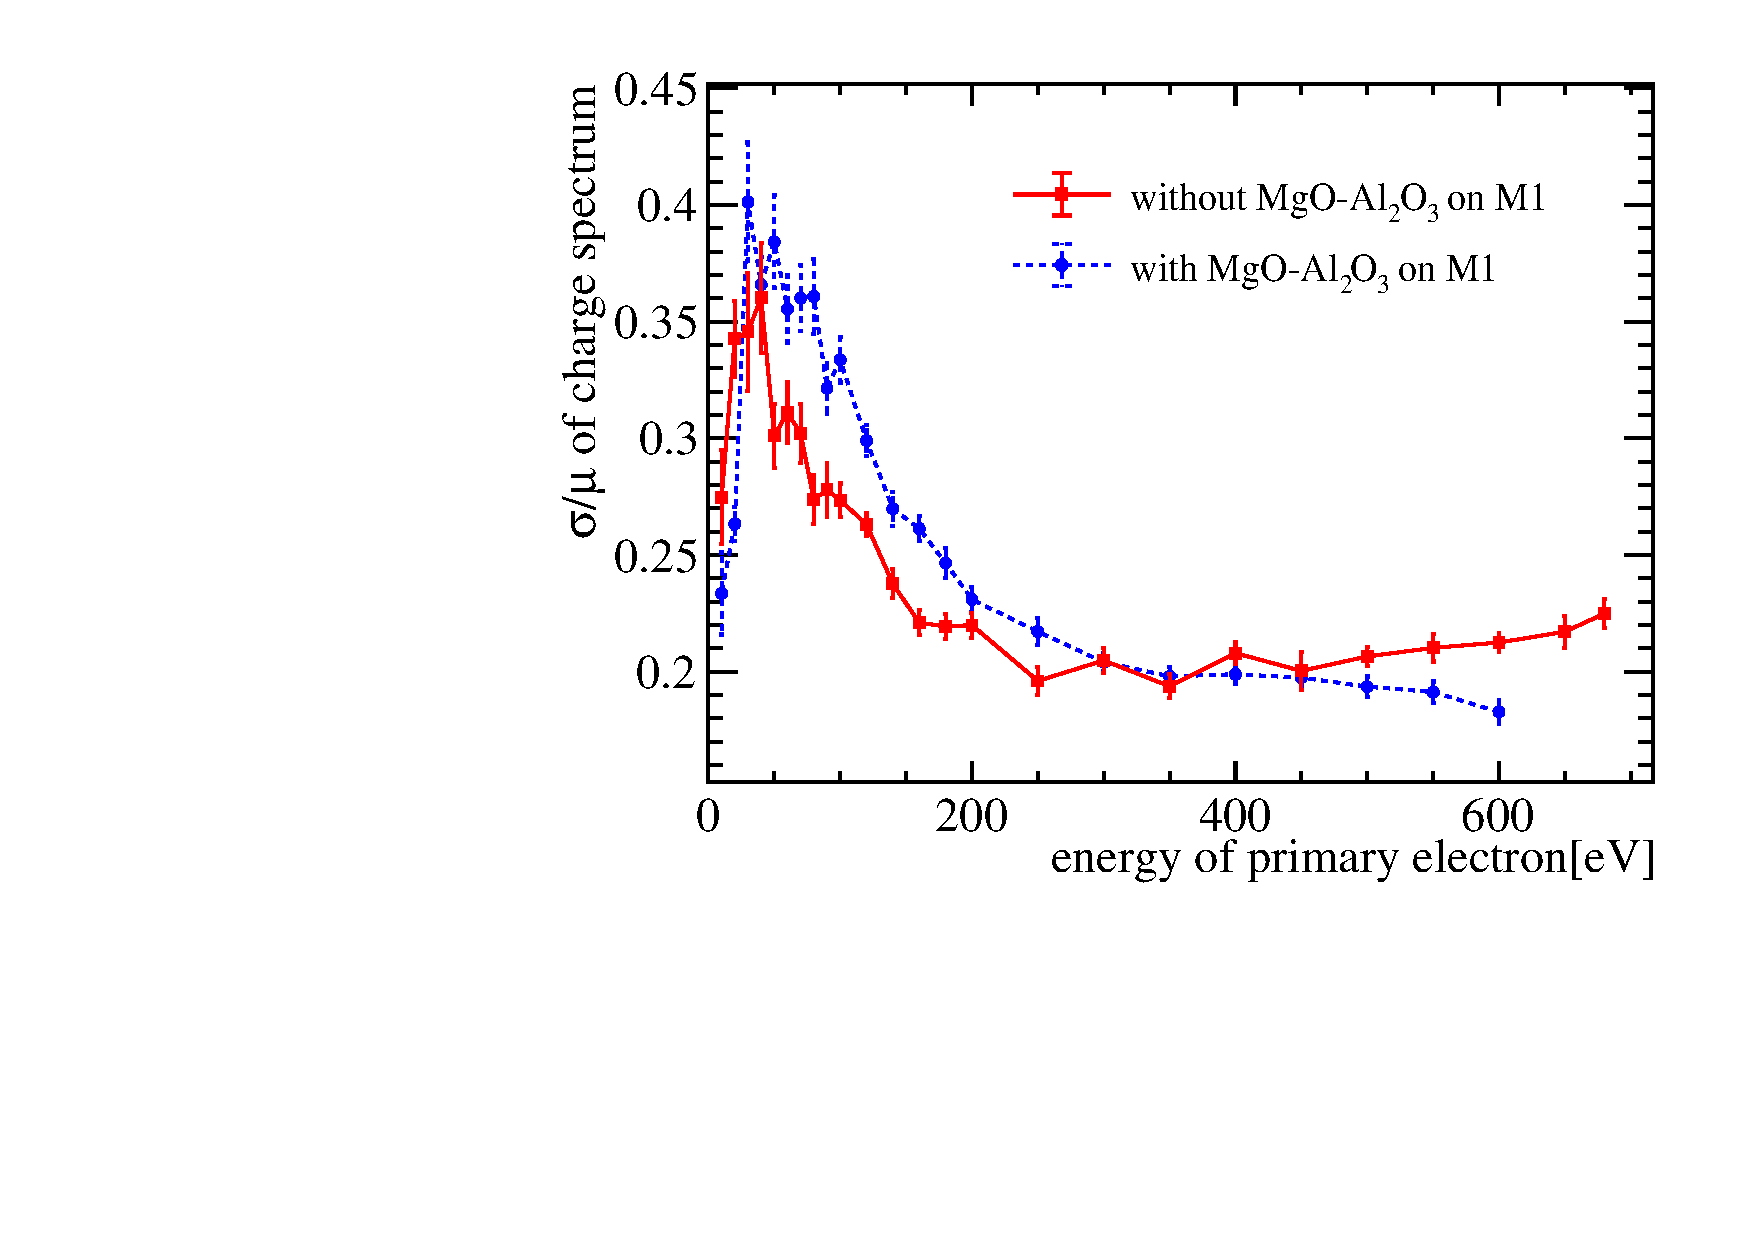
\includegraphics[width=0.9\textwidth]{PMTRelated/GTmodel/gain_sigmamu.pdf}
		\caption{}
		\label{fig:sigmamu}
	\end{subfigure}
	\caption{In \subref{fig:gain}, the mean value \(\mu\) rises as the incoming electron energy \(E_0\) goes up. Regarding \subref{fig:sigma}, the standard deviation \(\sigma\) varies with energy. The MCP - PMT with \ce{Al2O3}-\ce{MgO} deposited on \(\mathrm{M}1\) (represented by the red line) exhibits a variation trend similar to that of the one without such deposition (represented by the blue line). In \subref{fig:sigmamu}, the resolution \(\sigma/\mu\) increases in the range of 0 - \SI{50}{eV}, decreases between 50--\SI{400}{eV}, and after \SI{400}{eV}, for the MCP-PMT with \ce{Al2O3}-\ce{MgO} deposited on \(\mathrm{M}1\) (the blue line), there is a slight decline, while for the one without such deposition (the red line), there is a slight increase.
	}
	\label{fig:gaintest}
\end{figure}

\subsubsection{Charge-Spectra Decomposition}\label{sec:convolution}
The Furman model presented in Sec.~\ref{subsec:fuman} forecasts the energies of the secondaries. In our voltage-division experiment detailed in Sec.~\ref{sec:gain}, we measured the correlation between the MCP gain and the incident energies of electrons. We calculate the charge distribution using Monte Carlo following the flowchart shown in Fig.~\ref{fig:process}. In this research, we directed the laser at the apex of the photocathode hemisphere, and the PEs struck M1 with an incident angle of $\theta_0 = 0^\circ$. The intricate amplification process within the channels is characterized by the incident energy-dependent Gamma distributions $\varGamma(\alpha(E), \beta(E))$ as described in Sec.~\ref{gammapossion}. The values of $\alpha(E)$ and $\beta(E)$ are estimated based on the relationships of $\mu(E)$ and $\sigma(E)$ of an MCP-PMT without an \ce{Al2O3}-\ce{MgO} coating on the input electrode. This approach removes the influence of the surface mode.
\begin{figure}[!ht]
	\centering
	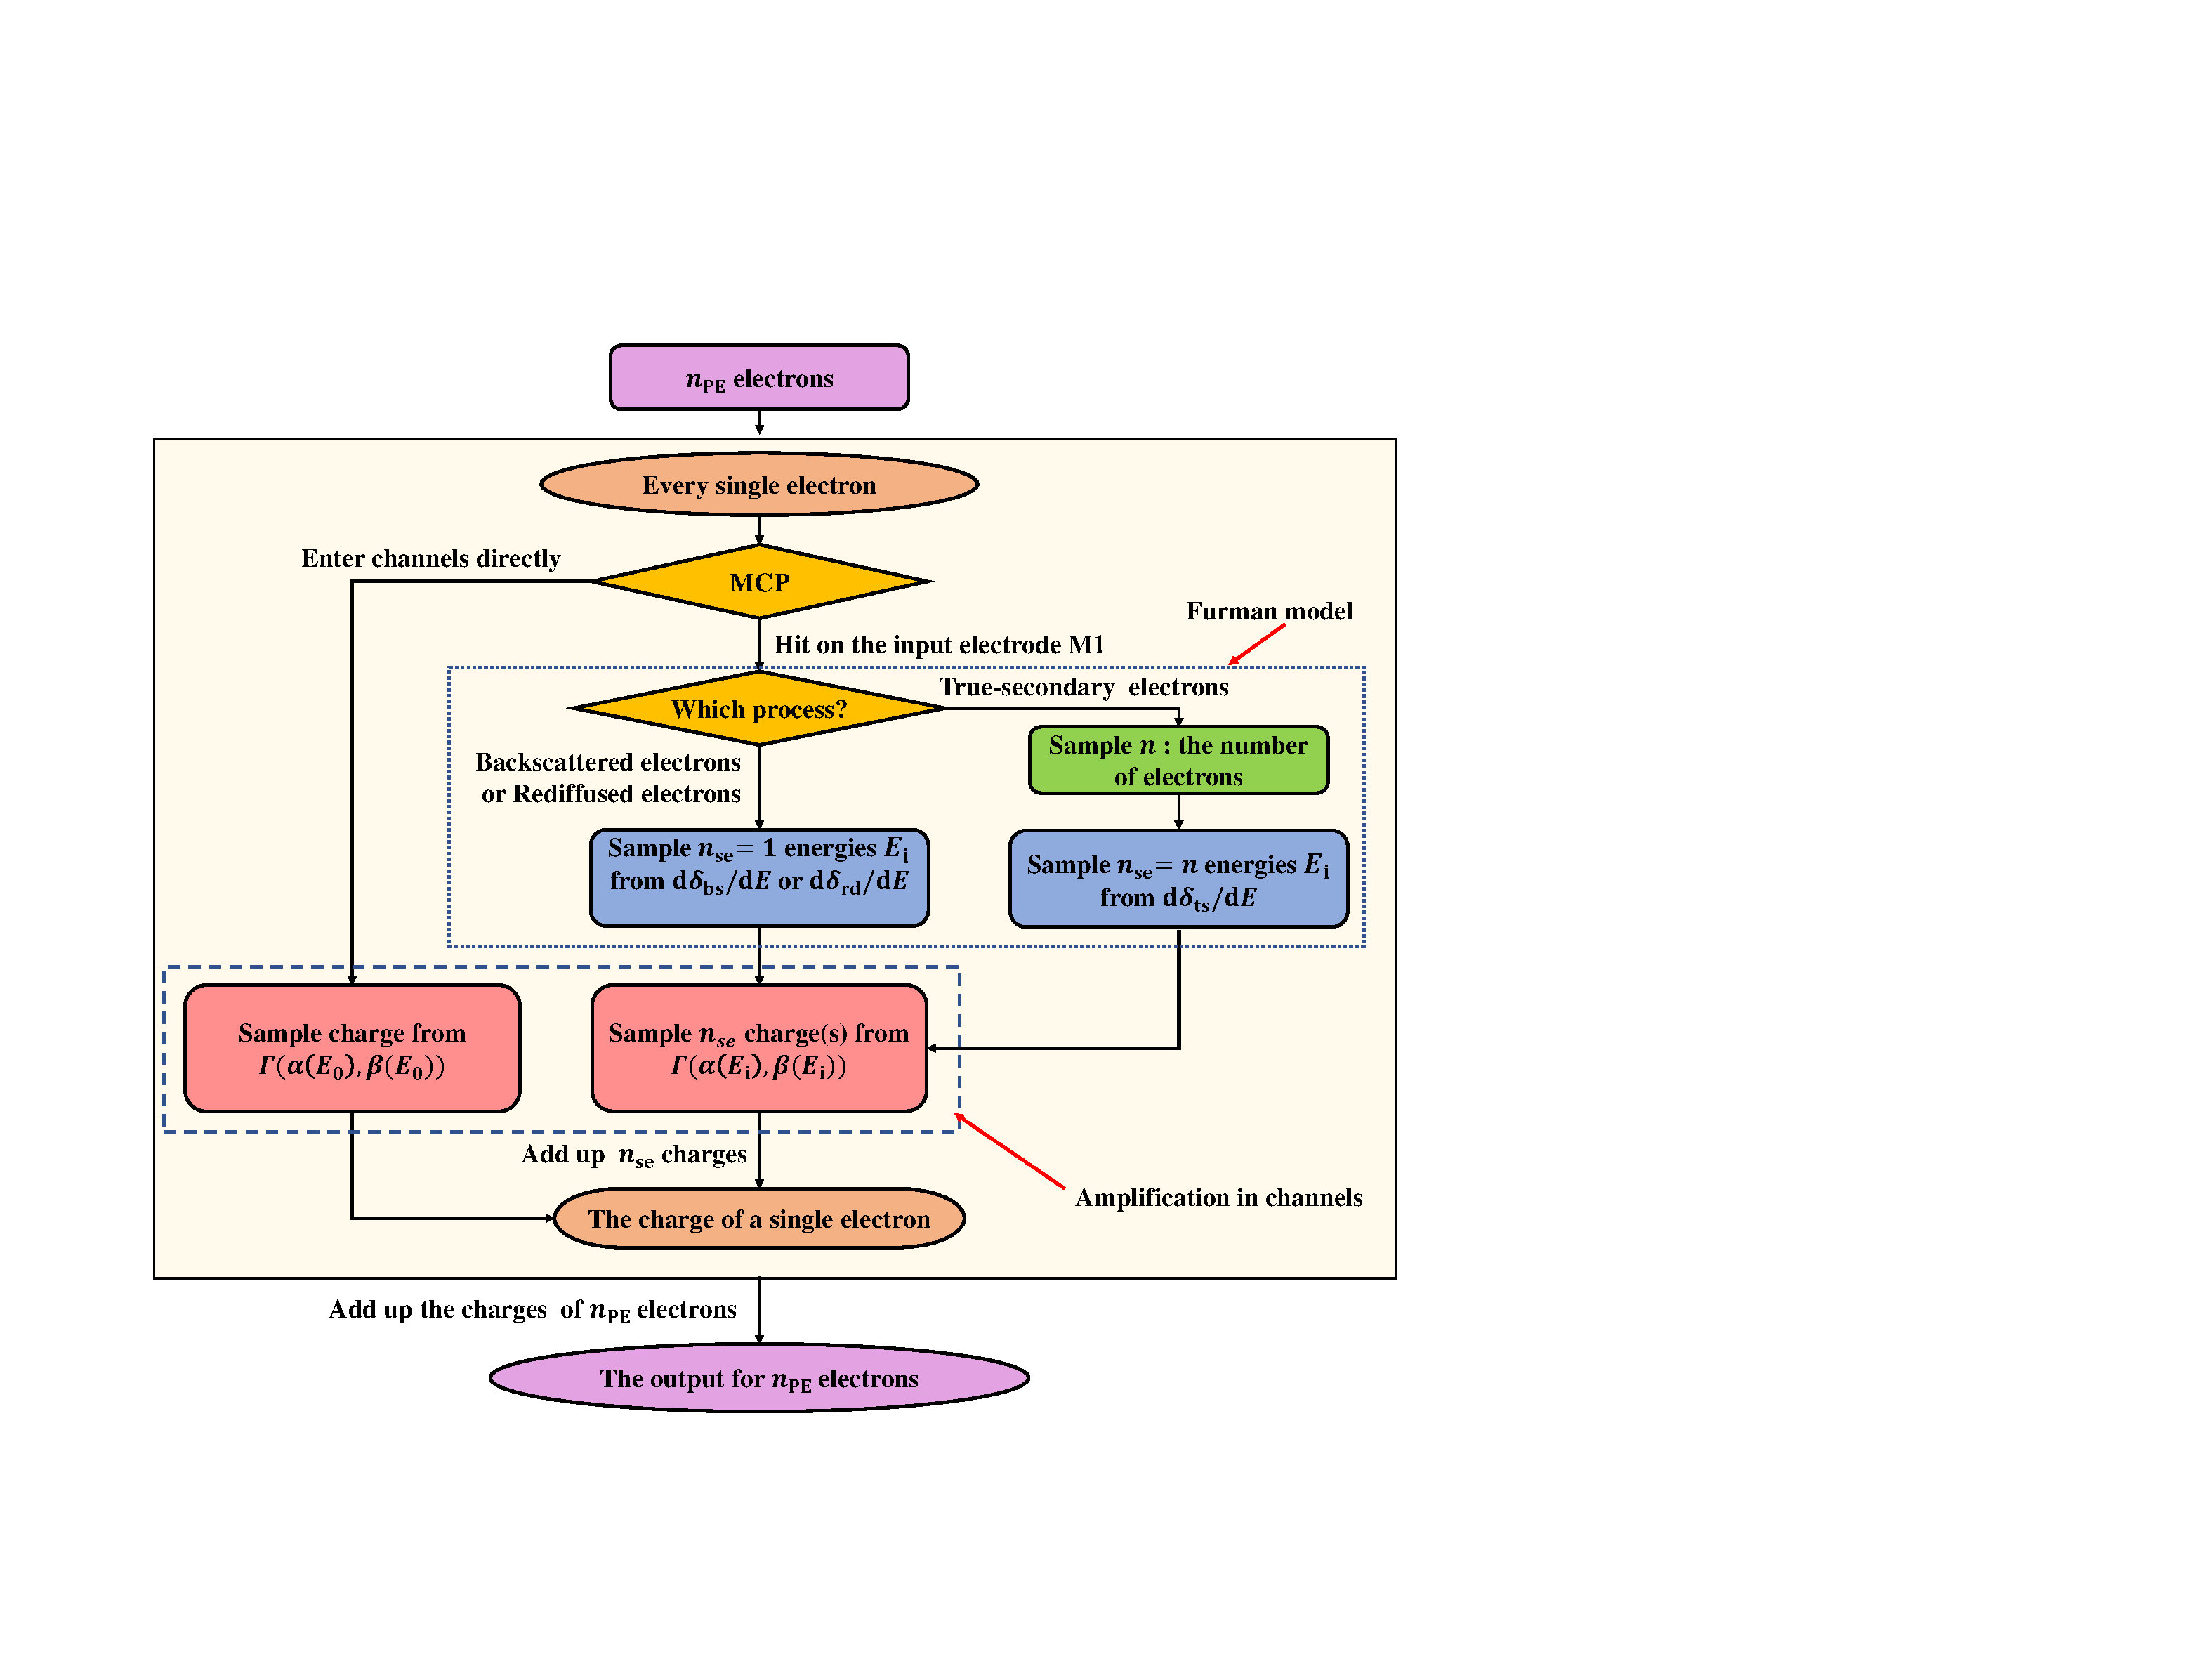
\includegraphics[width=\textwidth]{PMTRelated/GTmodel/process.pdf}
	\caption{The flowchart of Monte Carlo for calculating the charge spectrum is presented. The output charge is composed of \(n_\mathrm{PE}\) SER charges. In the channel mode, the PEs directly enter the channels, whereas in the surface mode, the PEs strike the input electrode. The energies of the \(n_\mathrm{se}\) secondaries in the surface mode are sampled according to the Furman model. The amplification in the channels is modeled using the incident energy-dependent Gamma distribution.
	}
	\label{fig:process}
\end{figure}
Considering the light intensity, we sample $n_{\mathrm{PE}}$ from the Poisson distribution multiple times. Then, we sum up $n_{\mathrm{PE}}$ SER charges for the output to obtain a spectrum. When sampling an SER charge, for a Bernoulli trial, we assign the probabilities of the channel and surface modes as $p$ and $1 - p$ respectively. The SER charge spectrum $f_{\text{MCP-PMT}}(Q)$ is given by the following equation:
\begin{equation}
	\label{eq:convolution}
	f_{\text{MCP-PMT}}(Q) = p f_{\mathrm{ch}}(Q)+(1 - p) f_{\mathrm{surf}}(Q)
\end{equation}
Here, $f_{\mathrm{ch}}(Q)$ and $f_{\mathrm{surf}}(Q)$ represent the charge distributions of the channel and surface modes. $f_{\mathrm{ch}}(Q)$ is set to \(f_\Gamma(Q; \alpha(E_0), \beta(E_0))\), where the incident energy is \SI{650}{eV}. The factors \(\alpha(E_0), \beta(E_0)\) are derived from $\mu(E_0)$ and $\sigma(E_0)$ without the \ce{Al2O3}-\ce{MgO} coating as shown in Fig.~\ref{fig:gaintest}.
According to the Furman model, $f_{\mathrm{surf}}(Q)$ is divided into three components corresponding to Eqs.~(\ref{eq:backscatter})--(\ref{eq:true}). Specifically, $f_{\mathrm{bs}}(Q)$ is for the back-scattered electrons, $f_{\mathrm{rd}}(Q)$ is for the rediffused electrons, and $f_{\mathrm{ts}}(Q)$ is for the true-secondary electrons.
\begin{equation}
	\label{eq:surface_3}
	\begin{aligned}
		f_{\mathrm{surf}}(Q) & = p_{\mathrm{bs}} f_{\mathrm{bs}}(Q) + p_{\mathrm{rd}} f_{\mathrm{rd}}(Q) + (1- p_{\mathrm{bs}} - p_{\mathrm{rd}}) f_{\mathrm{ts}}(Q)                     \\
		                     & = \delta_{\mathrm{bs}} f_{\mathrm{bs}}(Q) + \delta_{\mathrm{rd}} f_{\mathrm{rd}}(Q) + (1- \delta_{\mathrm{bs}} - \delta_{\mathrm{rd}}) f_{\mathrm{ts}}(Q) \\
	\end{aligned}
\end{equation}
In this context, $p_{\mathrm{bs}}$ and $p_{\mathrm{rd}}$ represent the mixture ratios. These ratios are decided by the composition and thickness of the surface emissive material, which can differ among the PMTs. According to Furman and Pivi in reference \cite{2002Probabilistic}, it is assumed that in the back-scattered mode and rediffused mode, only one electron is emitted. As a result, $\delta_{\mathrm{bs}} = p_{\mathrm{bs}}$ and $\delta_{\mathrm{rd}} = p_{\mathrm{rd}}$. During the calculation process, we set $\delta_{\mathrm{rd}} = 0.09$ and $\delta_{\mathrm{bs}} = 0.01$.
The energy of the back-scattered electron is approximately the same as that of the PEs in the channel mode. Consequently, the MCP gain for the back-scattered electron is also similar to that in the channel mode. In contrast, the energy of the rediffused electron is in the range of \SIrange{100}{600}{eV}, which is relatively lower. Due to the relatively slow increase of the gain in this energy range as shown in Fig.~\ref{fig:gain}, the charge after MCP multiplication for the rediffused electron is slightly smaller.
Both the back-scattered and rediffused electrons contribute a single electron each. In the charge spectra, they are virtually indistinguishable from the channel mode. This degeneracy phenomenon is concisely presented in Eq.~\eqref{eq:gammaTweedie}.
\begin{equation}
	\label{eq:gammaTweedie}
	\begin{aligned}
		f_{\text{MCP-PMT}}(Q) & = p f_{\mathrm{ch}}(Q) + (1-p) f_{\mathrm{surf}}(Q)                                                                                                                                    \\
		                      & = p f_{\mathrm{ch}}(Q)+(1-p) [\delta_{\mathrm{bs}} f_{\mathrm{bs}}(Q) + \delta_{\mathrm{rd}} f_{\mathrm{rd}}(Q) + (1- \delta_{\mathrm{bs}} - \delta_{\mathrm{rd}}) f_{\mathrm{ts}}(Q)] \\
		                      & = [p + (1-p)(\delta_{\mathrm{bs}} + \delta_{\mathrm{rd}})] f_{\mathrm{ch}}(Q) + (1-p)(1-\delta_{\mathrm{bs}} - \delta_{\mathrm{rd}})f_{\mathrm{ts}}(Q)
	\end{aligned}
\end{equation}
In this situation, the spectra \(f_{\mathrm{ch}}(Q)\), \(f_{\mathrm{rd}}(Q)\), and \(f_{\mathrm{bs}}(Q)\) are combined into \(f_{\mathrm{ch}}(Q)\). However, Eq.~(\ref{eq:gammaTweedie}) is not complete. We need to take into account the scenario where the secondaries strike the MCP surface once more. The round trip does not introduce additional energy. A back-scattered or rediffused secondary is amplified in a manner that is essentially the same as a primary PE. On the other hand, a true-secondary electron has an energy that is too low to undergo multiplication again. Consequently, \(p_0\), which is the net contribution to \(f_{\mathrm{ch}}(Q)\), forms a geometric series.
\begin{equation}
	\label{eq:p0}
	p_0 = p \sum_{{i}=0}^\infty [(1-p) (\delta_{\mathrm{bs}} + \delta_{\mathrm{rd}})]^{i} = \frac{p}{1 - (1-p) (\delta_{\mathrm{bs}} + \delta_{\mathrm{rd}})}
\end{equation}
and \(f_{\mathrm{ts}}(Q)\) gets \(\frac{(1-p)(1-\delta_{\mathrm{bs}} - \delta_{\mathrm{rd}})}{1 - (1-p) (\delta_{\mathrm{bs}} + \delta_{\mathrm{rd}})}\) or \(1-p_0\).
Eq.~(\ref{eq:gammaTweedie}) is remarkably reduced to
\begin{equation}
	\label{eq:1}
	f_{\text{MCP-PMT}}(Q) = p_0 f_{\mathrm{ch}}(Q) + (1-p_0) f_{\mathrm{ts}}(Q).
\end{equation}

For the true-secondary electrons, the count $n$ follows a Poissonian. The sum of the sampled $n$ charges serves as the output \(Q_{\mathrm{ts}}\),
\begin{equation}
	\label{eq:ts_all}
	\begin{aligned}
		 & Q_{\mathrm{ts}} = \sum_{i=1}^{n} Q_{i}            \\
		 & n \sim \mathrm{\pi}(\delta_{\mathrm{ts}}')        \\
		 & Q_{i} \sim \varGamma[\alpha(E_{i}), \beta(E_{i})] \\
	\end{aligned}
\end{equation}
where \(E_{i}\) is sampled from Eq.~(\ref{eq:true}).
The values of \(\alpha(E_{i})\) and \(\beta(E_{i})\) are derived from \(\mu(E_{i})\) and \(\sigma(E_{i})\) as presented in Fig.~\ref{fig:gaintest}. For the sake of comprehensiveness, \(\delta_\mathrm{ts} = (1-\delta_{\mathrm{bs}} - \delta_{\mathrm{rd}})\delta_{\mathrm{ts}}'\) represents the ratio of the electric current of the true-secondary electrons to that of the primary electrons. The charge spectra corresponding to different values of \(n\) are depicted in Fig.~\ref{fig:true_n}. Owing to the relatively lower energies of the secondary electrons, their charges are smaller. Differentiating each charge formed at the anode is a difficult task because multiple secondary electrons enter the MCP channels at the same time. A larger value of \(n\) leads to a greater charge.
\begin{figure}[htbp]
	\begin{subfigure}{0.5\textwidth}
		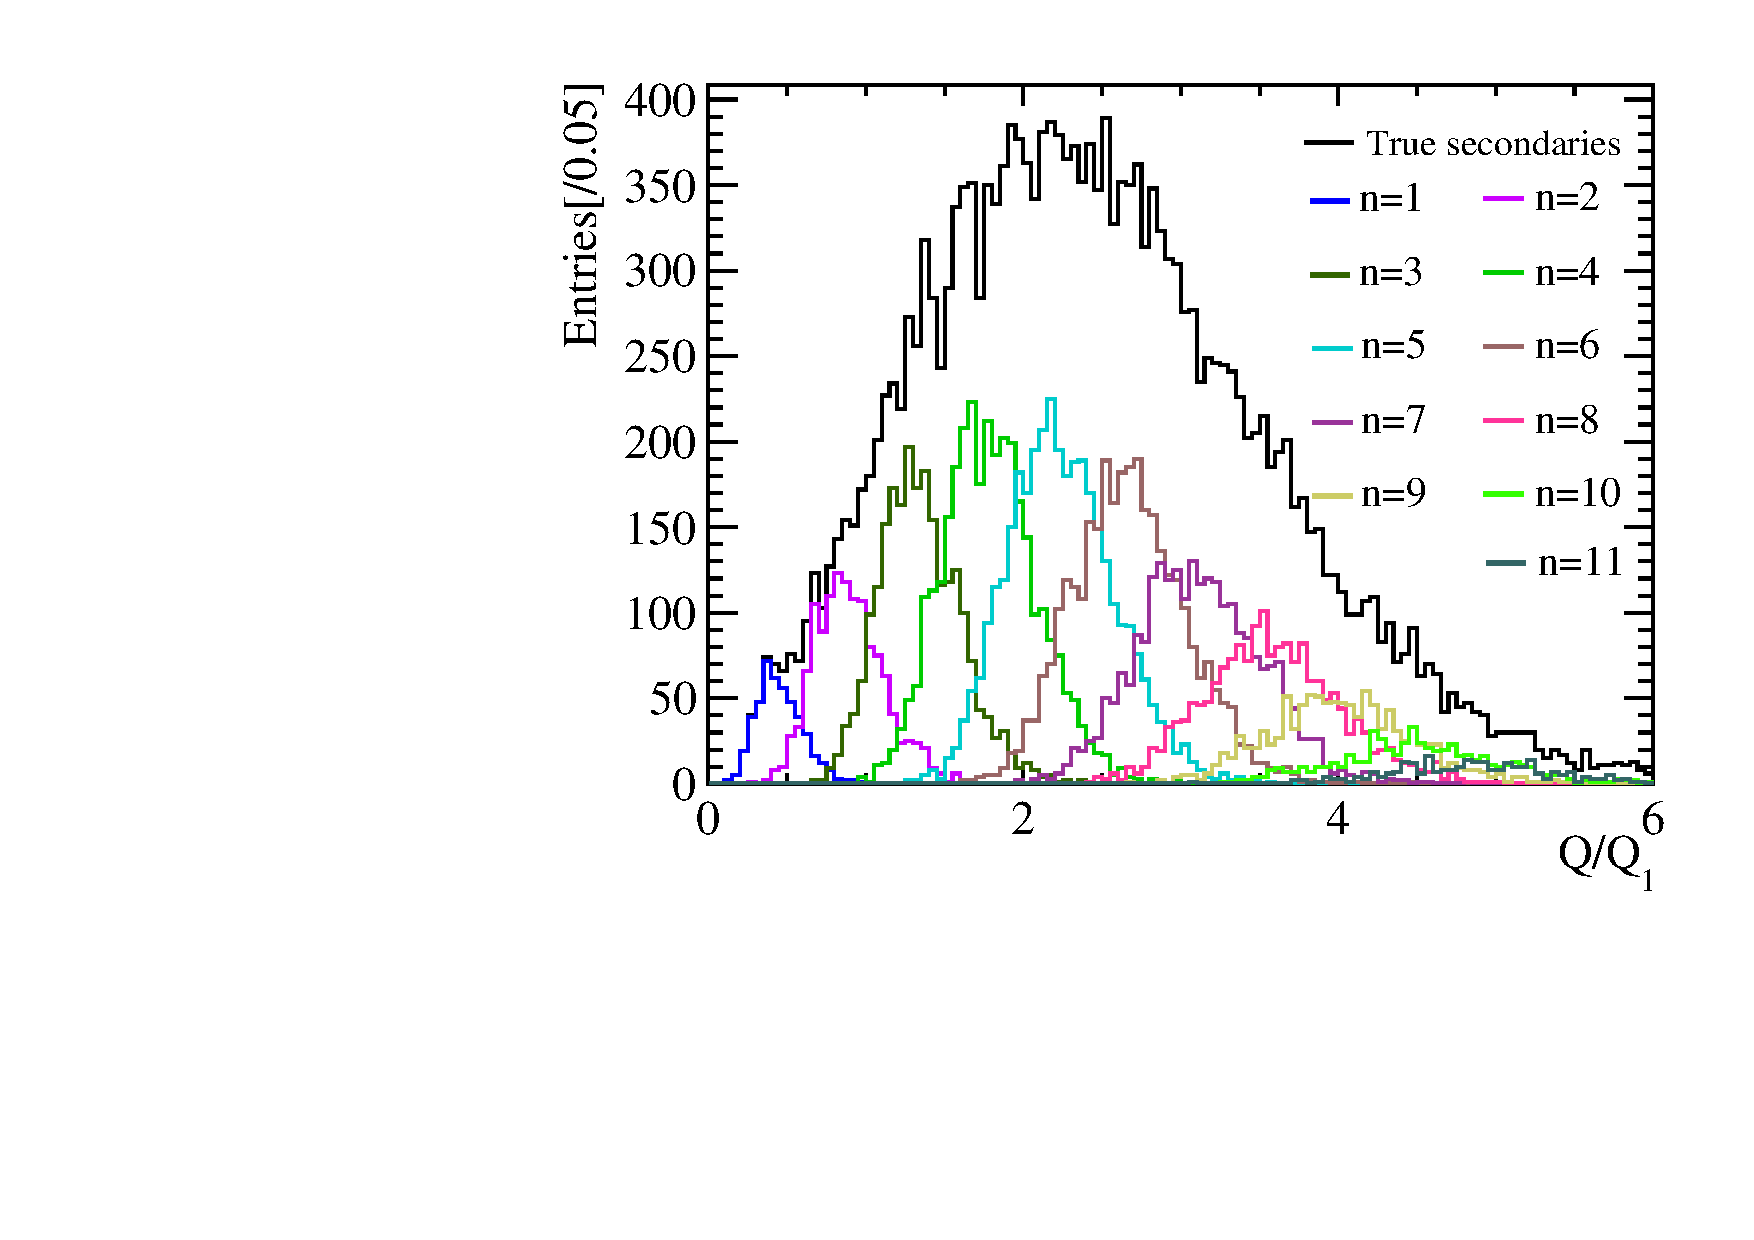
\includegraphics[width=0.9\textwidth]{PMTRelated/GTmodel/true_all.pdf}
		\caption{}
		\label{fig:true_n}
	\end{subfigure}%
	\hfill
	\begin{subfigure}{0.5\textwidth}
		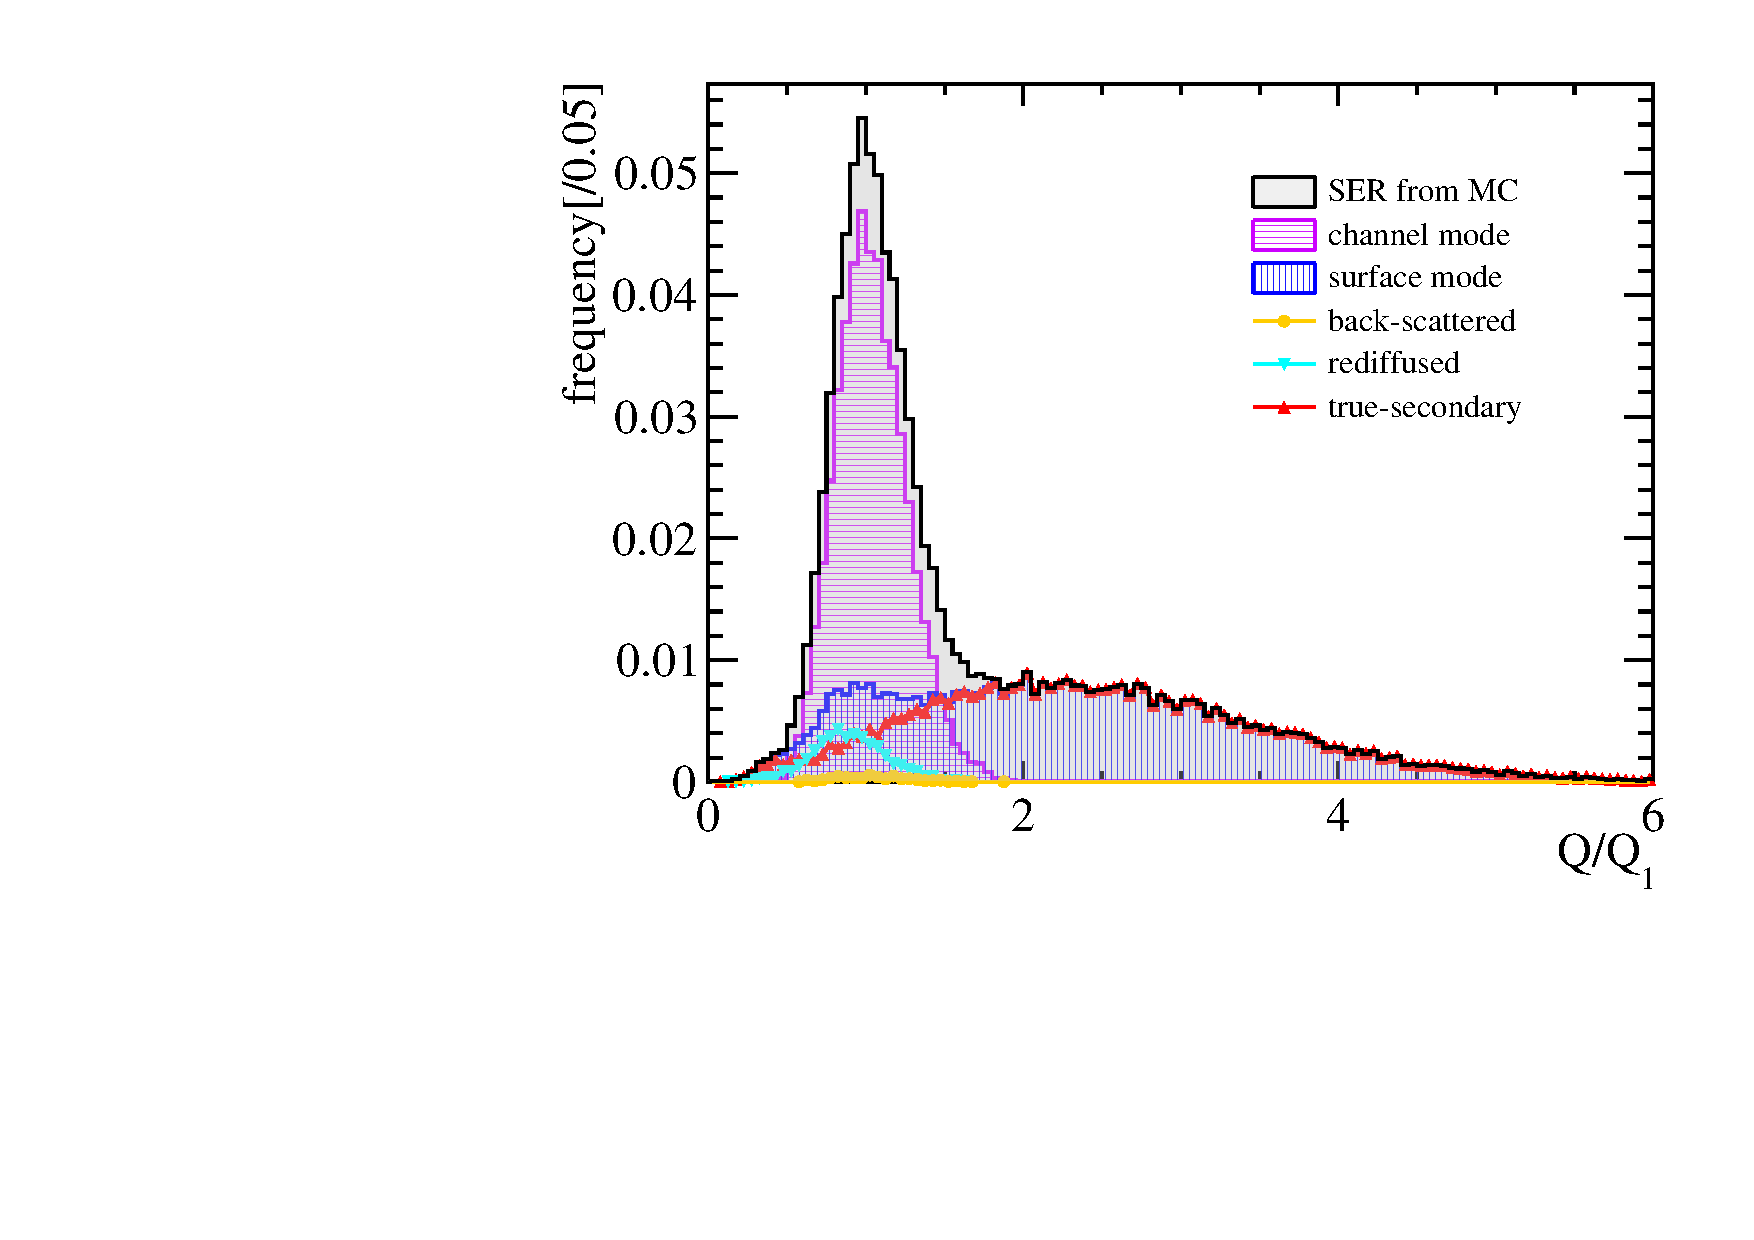
\includegraphics[width=0.9\textwidth]{PMTRelated/GTmodel/allmode.pdf}
		\caption{}
		\label{fig:allmode}
	\end{subfigure}
	\caption{\subref{fig:true_n}: In the MC calculation, when $\delta_{\mathrm{ts}}' = 5.5$ and $p_0 = 0.55$, this shows the charge distribution of the true-secondary electrons mode. The black histogram represents the sum of all distributions. \subref{fig:allmode}: The charge distribution formed in the channel mode is centered around the peak. Meanwhile, the tail part is mainly produced by the true-secondary electrons in the surface mode. }
\end{figure}

Fig.~\ref{fig:allmode} presents a typical decomposition of the SER charge spectra. The jumbo charges, which are also referred to as the “long tail,” result from the true secondaries generated by the surface mode.

\subsection{Parameter Extraction from Data}\label{subsec:chitest}
From Eq.~(\ref{eq:1}) and (\ref{eq:ts_all}), it can be clearly seen that $\delta_{\mathrm{ts}}'$ and \(p_0\) have a substantial influence on the SER charge distribution, as shown in Fig.~\ref{fig:tsp}. To determine these two parameters, we utilize the MCP - PMT test data provided by Zhang et al.~\cite{Zhang:2023ued}.
\begin{figure}[htbp]
	\centering
	\begin{subfigure}{0.5\textwidth}
		\centering
		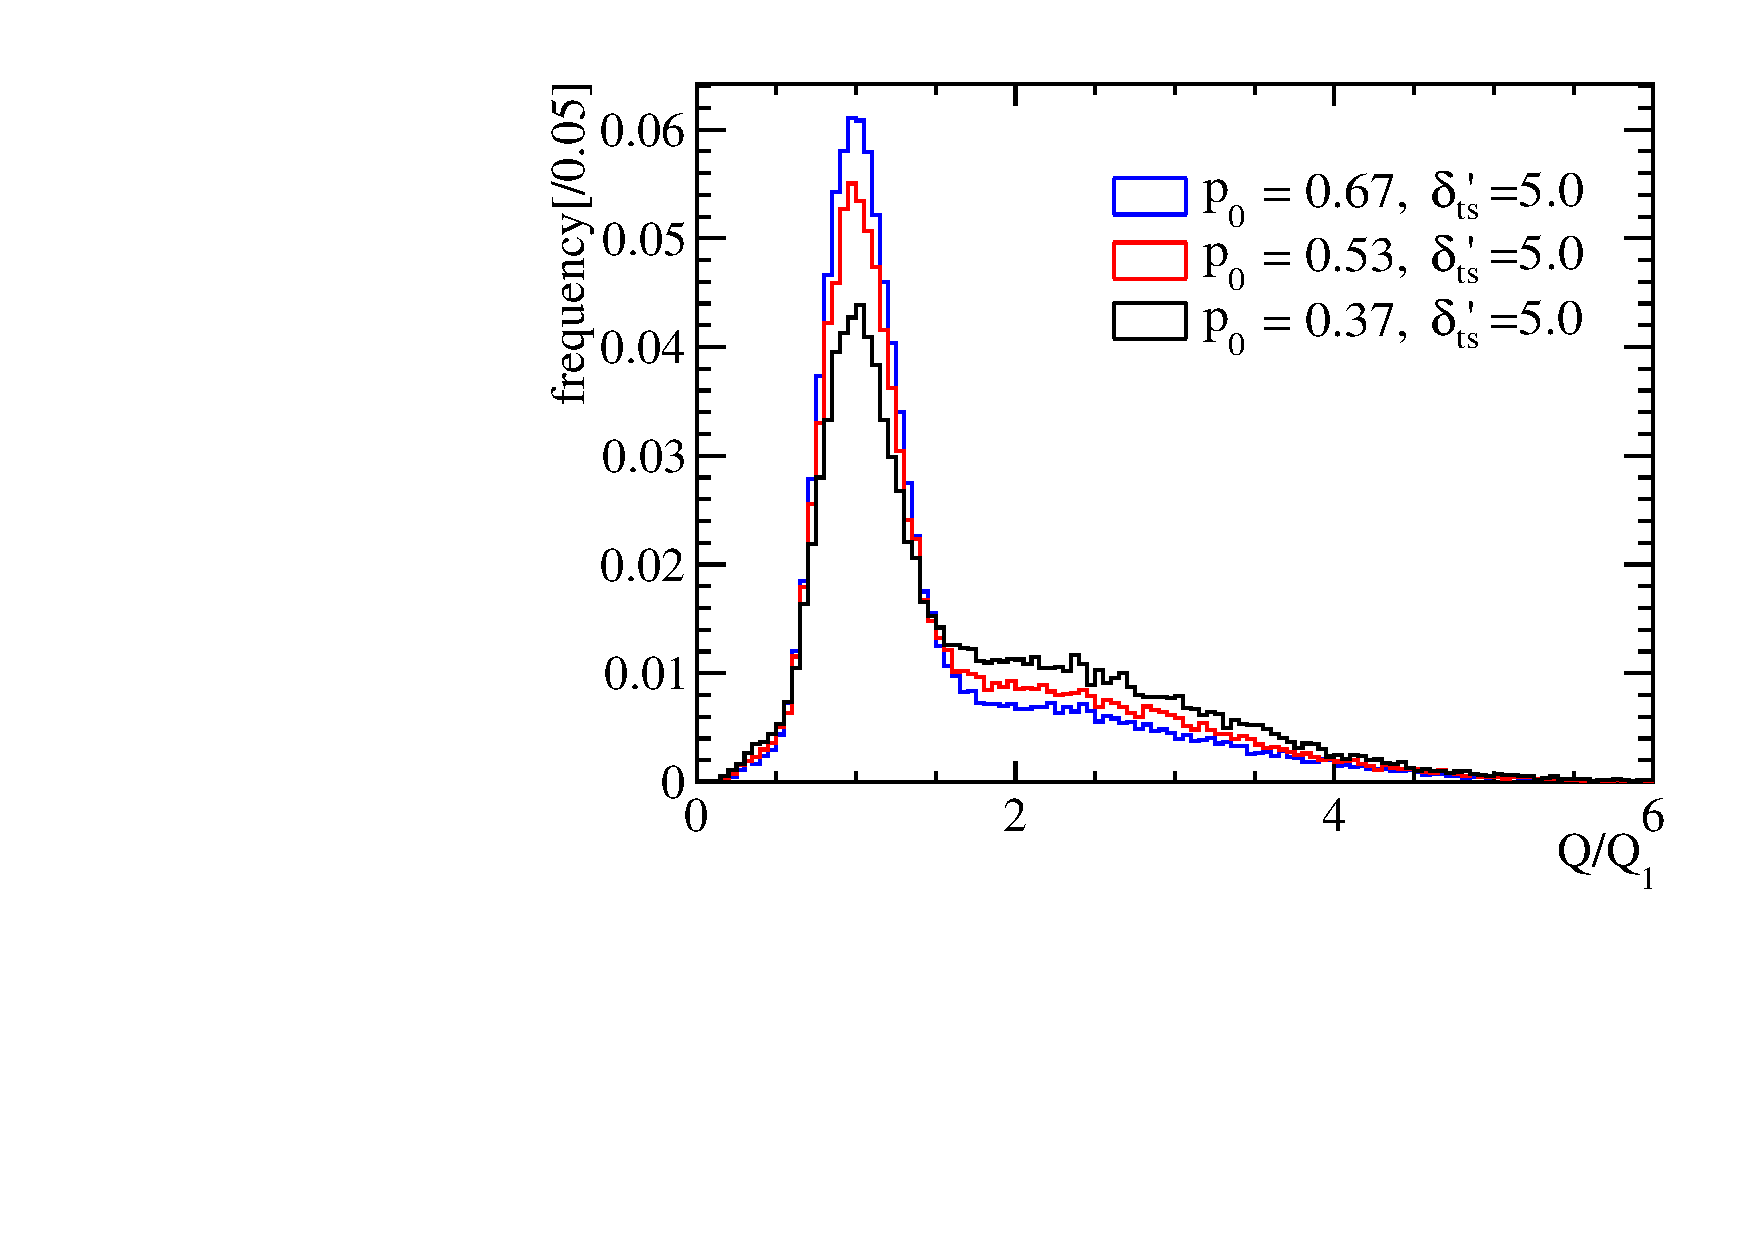
\includegraphics[width=0.9\textwidth]{PMTRelated/GTmodel/p.pdf}
		\caption{}
		\label{fig:p}
	\end{subfigure}%
	\hfill
	\begin{subfigure}{0.5\textwidth}
		\centering
		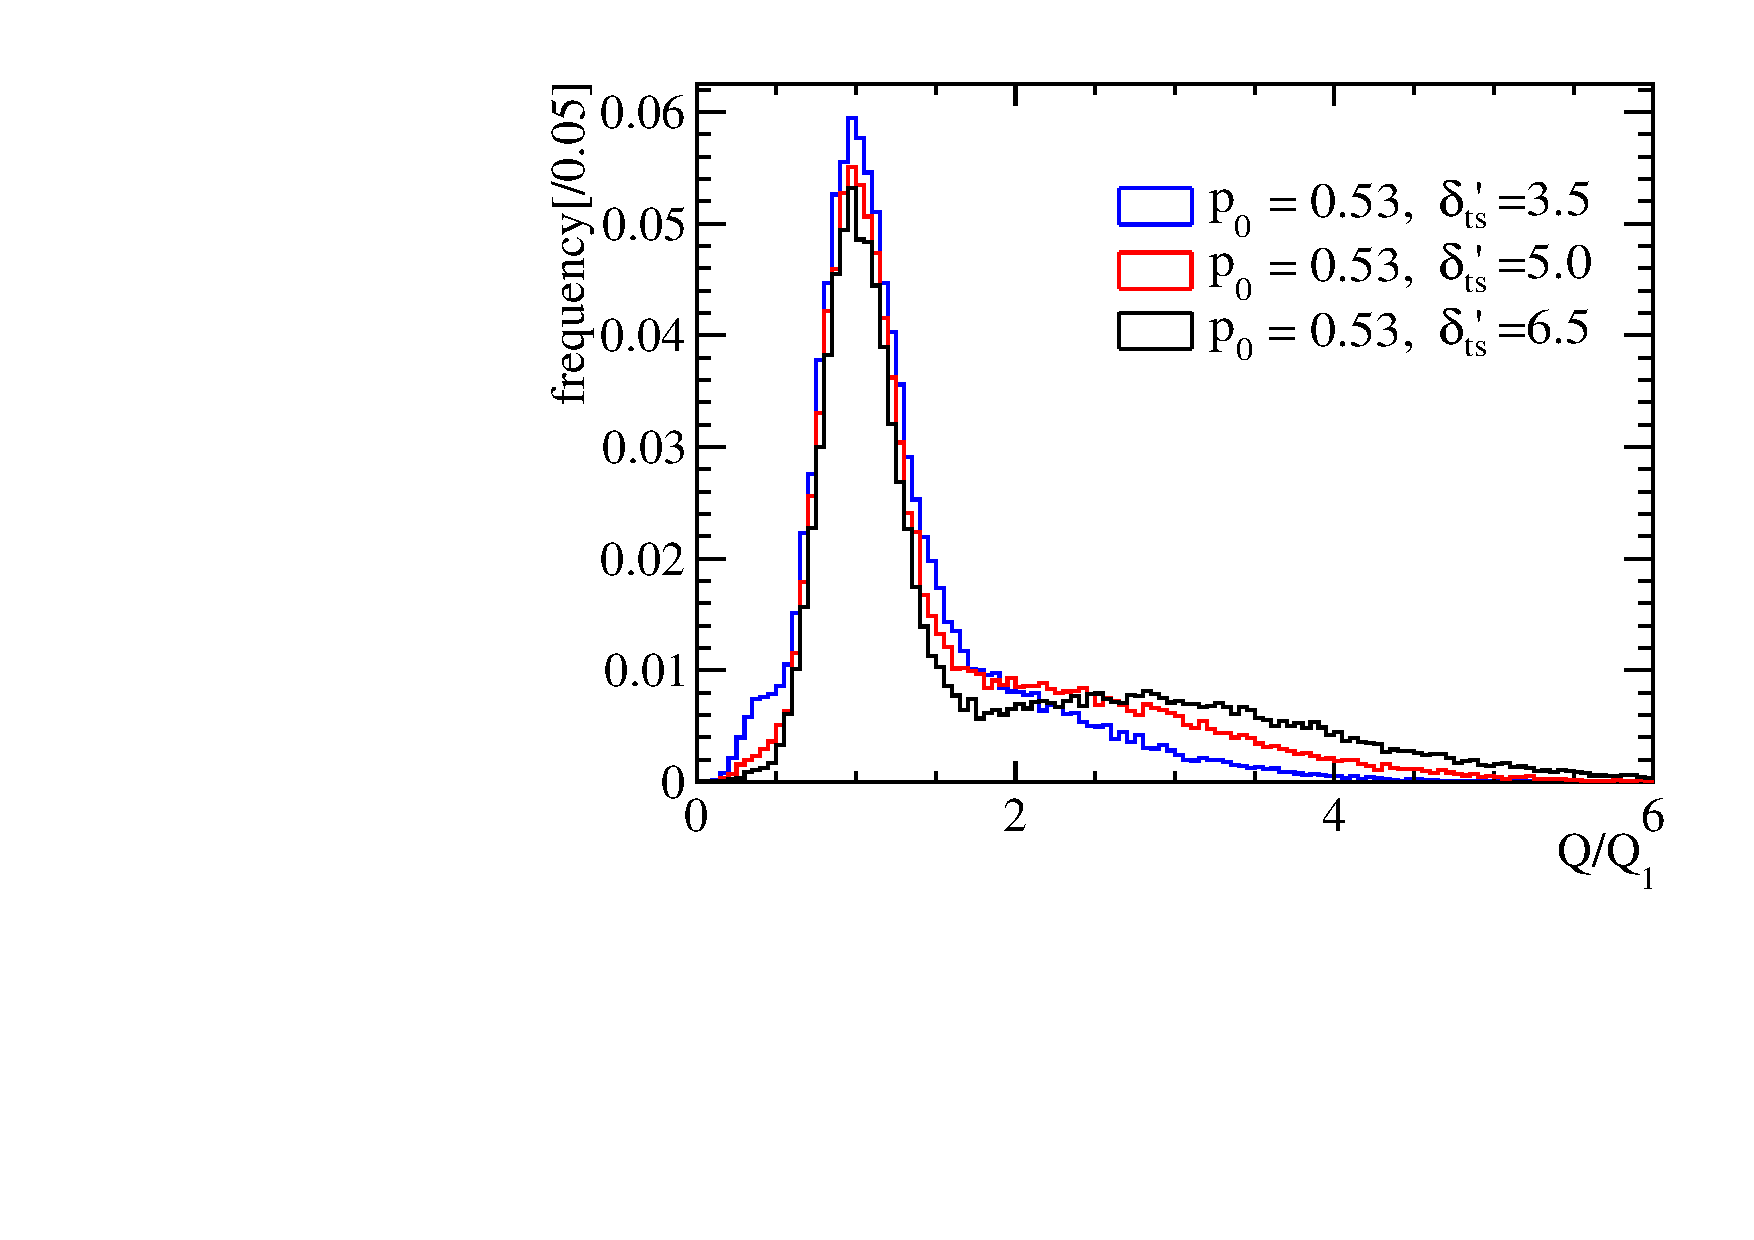
\includegraphics[width=0.9\textwidth]{PMTRelated/GTmodel/ts.pdf}
		\caption{}
		\label{fig:ts}
	\end{subfigure}
	\caption{The shape of the SER charge spectrum obtained from MC is affected by $\delta_{\mathrm{ts}}'$ and $p_0$. When $\delta_{\mathrm{ts}}'$ rises, the tail region extends more. When $p_0$ increases, the height of the principal peak region goes up, and the tail becomes  narrower.
	}
	\label{fig:tsp}
\end{figure}

We conduct a chi-square test for each pair of the predicted and measured charge distributions. The same binning approach is used to divide these two histograms into \(r\) bins. Let the number of entries in the \(i\)-th bin be \(n_i\) and \(m_{i}\), where \(N=\sum_{i = 1}^{r}n_{i}\) and \(M=\sum_{i = 1}^{r}m_{i}\). As stated in reference \cite{2006Comparison}, the chi-square test serves to show the similarity between the two histograms.
\begin{equation}
	\label{eq:chi}
	\begin{aligned}
		\chi^2_{r-1} & =\sum_{{i}=1}^r \frac{\left(n_{i}-N \hat{k}_{i}\right)^2}{N \hat{k}_{i}}+\sum_{{i}=1}^r\frac{\left(m_{i}-M \hat{k}_{i}\right)^2}{M \hat{k}_{i}} \\
		             & =\frac{1}{M N} \sum_{{i}=1}^r\frac{\left(M n_{i}-N m_{i}\right)^2}{n_{i}+m_{i}}
	\end{aligned}
\end{equation}
where \(\hat{k}_{i}=\frac{n_{i}+m_{i}}{N+M}\).

The \(\chi^2_{r - 1}\) values are scanned across the \((p_0,\delta_{\mathrm{ts}}')\) grid. An example is presented in Fig.~\ref{fig:cour}. We adopt a linear model~\cite{Gelman_Hill_2006} to smooth the approximately parabolic relationship between the \(\chi^2_{r - 1}\) and \((p_0, \delta_{\mathrm{ts}}')\). Subsequently, we extract the \((\hat{p}_0, \hat{\delta}_{\mathrm{ts}}')\) values that minimize \(\chi^2_{r - 1}\), along with intervals at \SI{68.3}{\percent} confidence levels~\cite{cowan1997statistical}.

\begin{figure}[htbp]
	\centering
	\begin{subfigure}{0.5\textwidth}
		\centering
		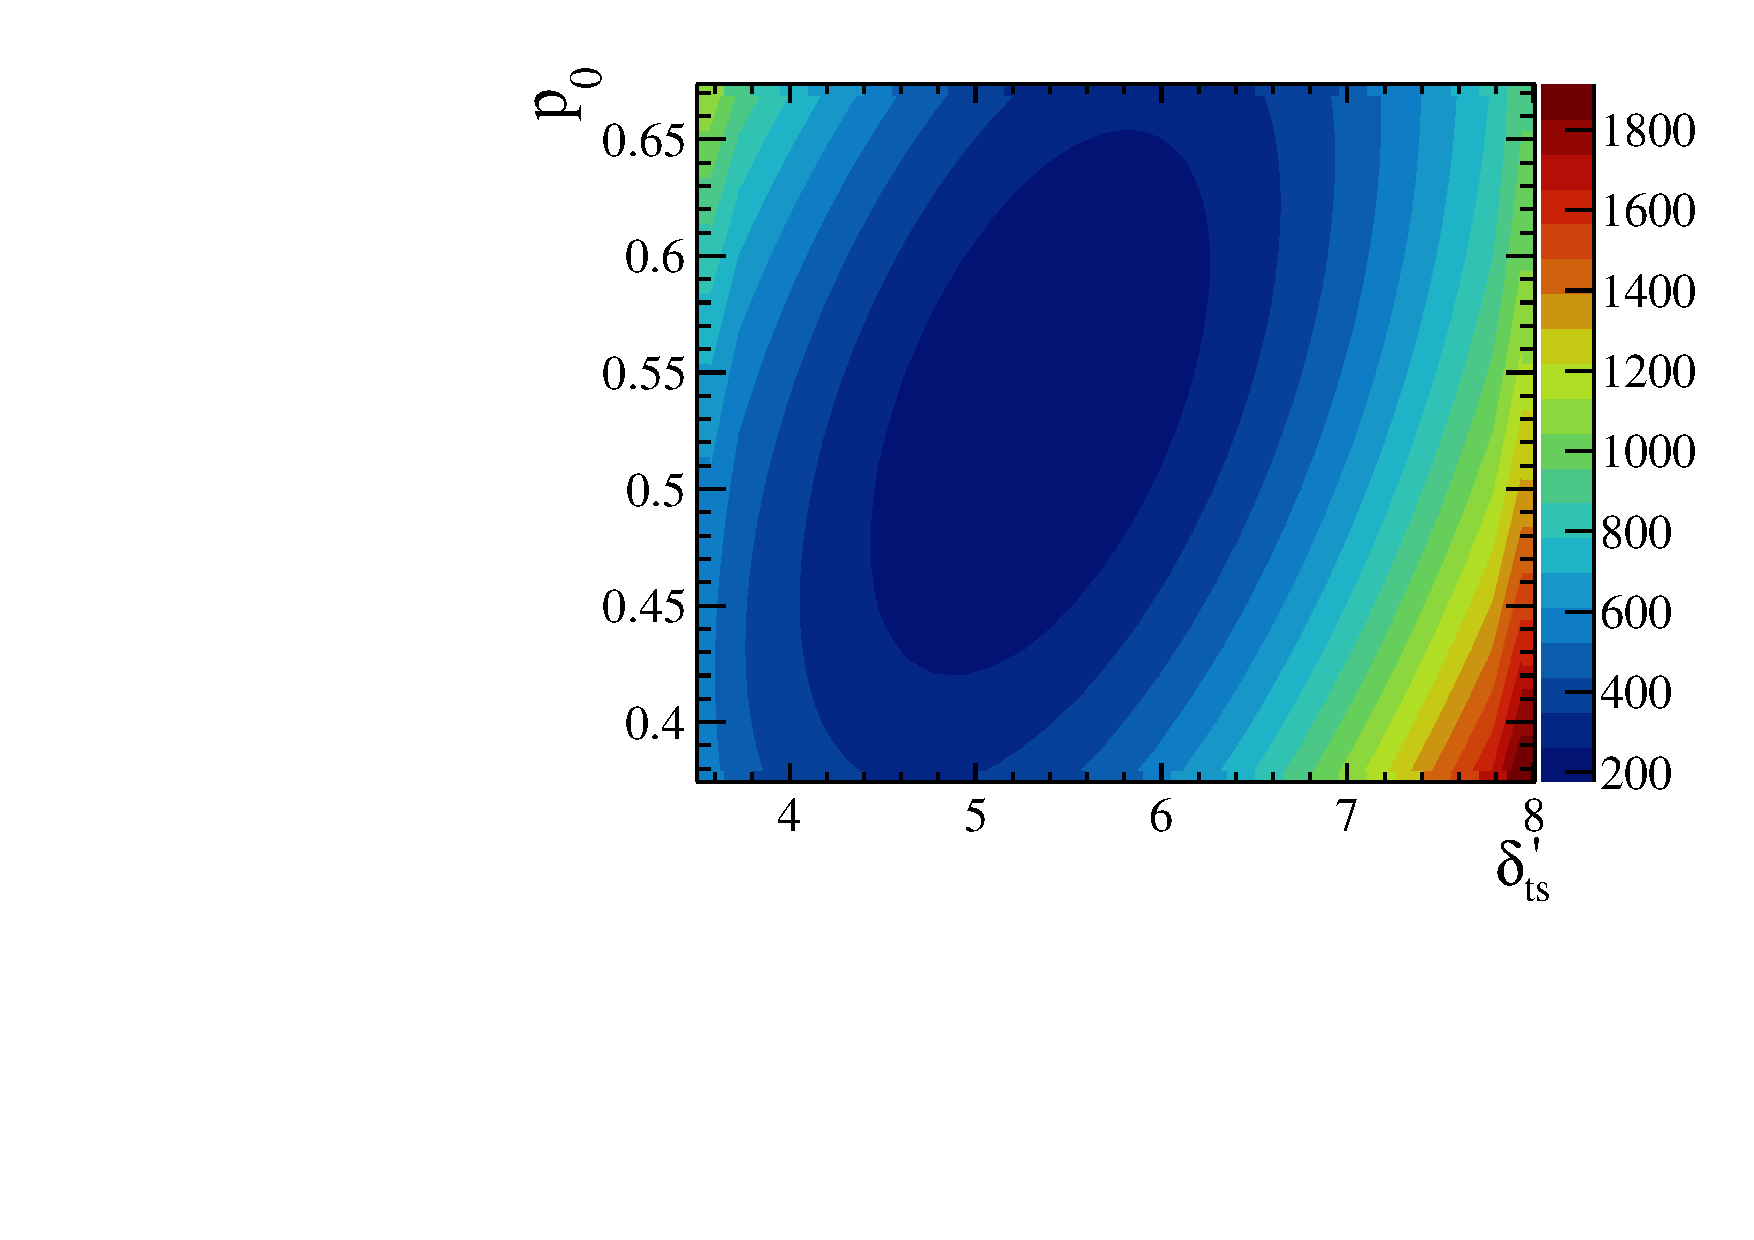
\includegraphics[width=0.9\textwidth]{PMTRelated/GTmodel/cour.pdf}
		\caption{}
		\label{fig:cour}
	\end{subfigure}%
	\hfill
	\begin{subfigure}{0.5\textwidth}
		\centering
		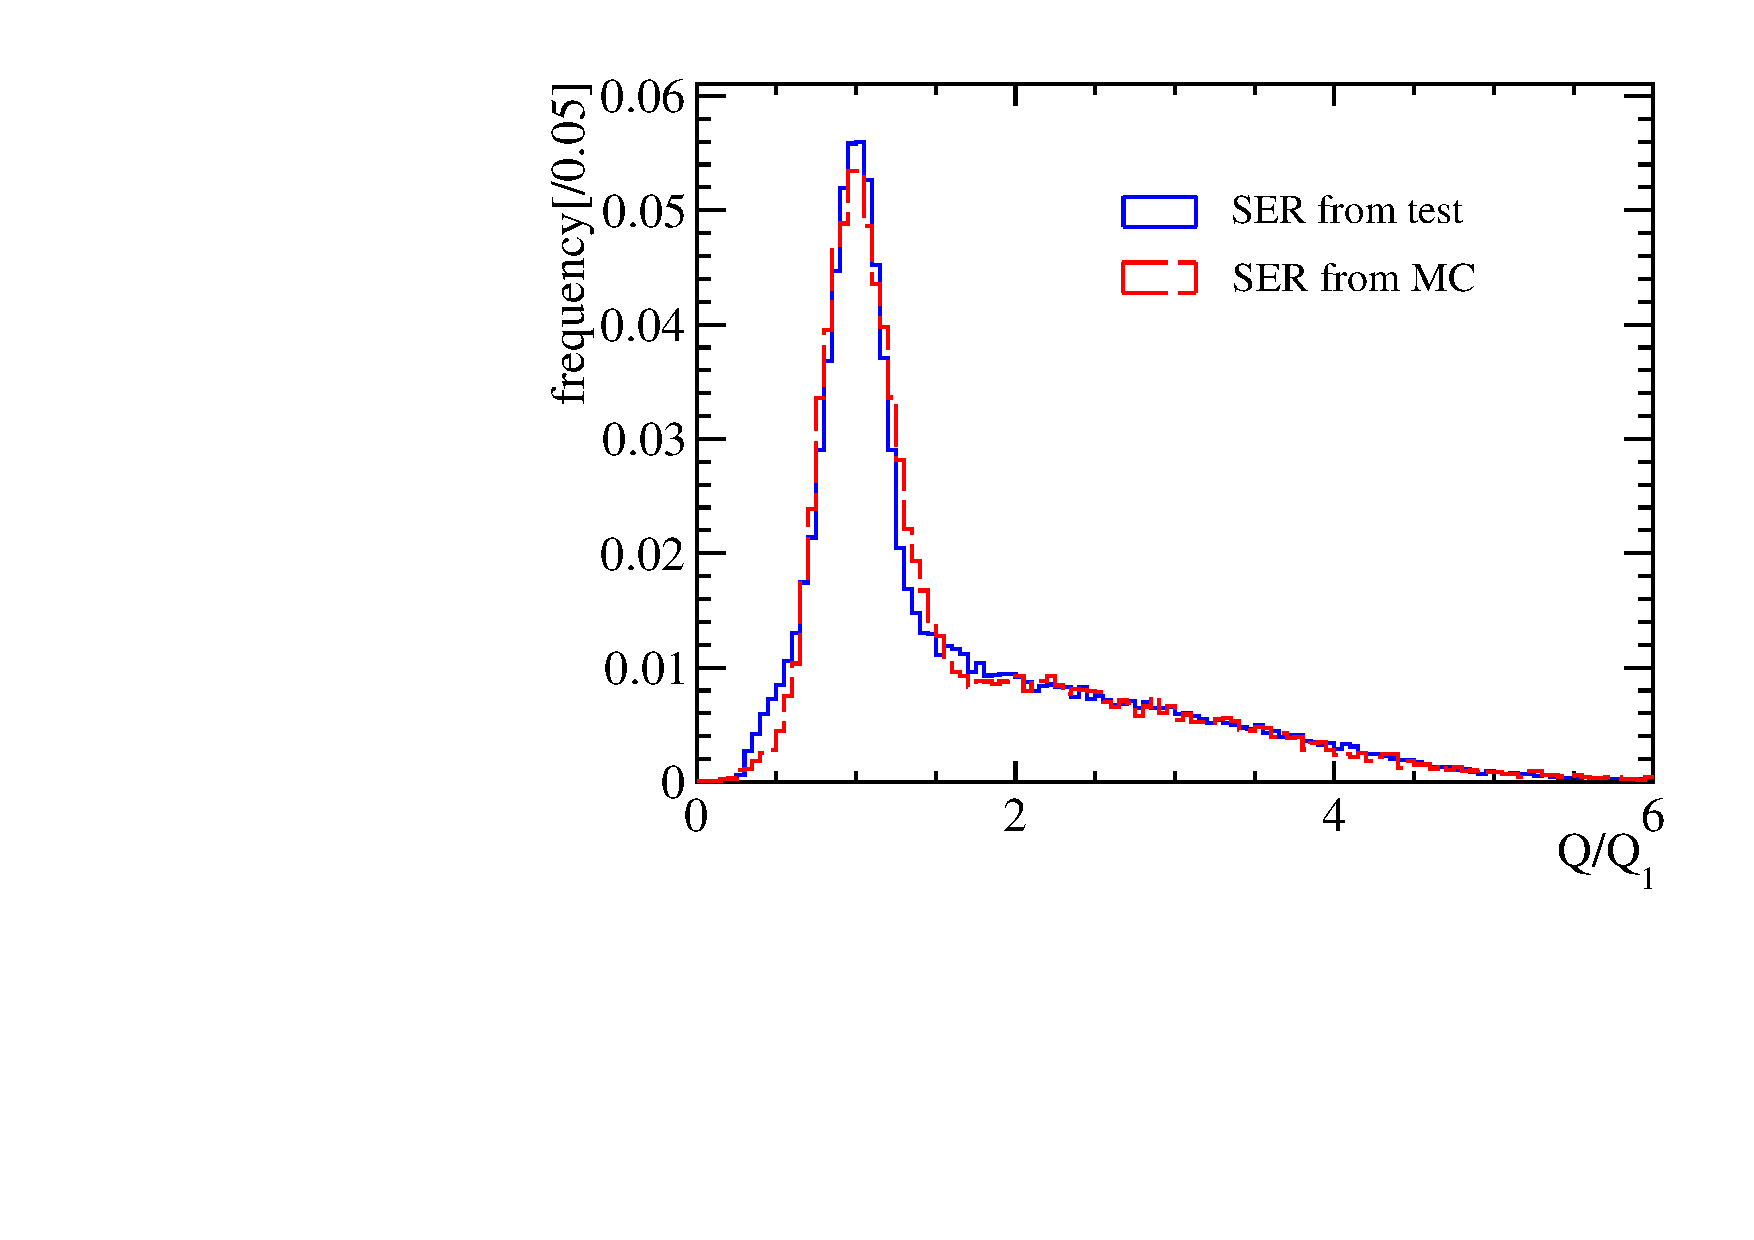
\includegraphics[width=0.9\textwidth]{PMTRelated/GTmodel/hist.pdf}
		\caption{}
		\label{fig:hist}
	\end{subfigure}
	\caption{The plot in \subref{fig:cour} is a contour plot of the chi-square test. Here, $p_0$ and $\delta_{\mathrm{ts}}'$ are used as parameters, and the chi-square values represent the height. The plot in \subref{fig:hist} shows an example of the Monte Carlo (MC) histogram (depicted by the red line) and the histogram obtained from the test (represented by the blue line).
	}
	\label{fig:chi}
\end{figure}

The scatter plot of $\hat{\delta}_{\mathrm{ts}}'$ versus $\hat{p}_0$ for 9 MCP-PMTs shown in Fig.~\ref{fig:true_p} does not suggest a strong correlation. This is because they are decided by independent manufacturing steps. On an average basis, the value of $\delta_{\mathrm{ts}}'$ is 5.979 and that of $p_0$ is 0.5341. % rd=0.09,bs=0.01. 
The PEs of the channel, back-scattered, and rediffused surface modes make up \SI{53.41}{\percent}, forming the peak. For each of the remaining cases, when hitting the surface, it induces 5.979 true-secondary electrons on average.
\begin{figure}[htbp]
	\centering
	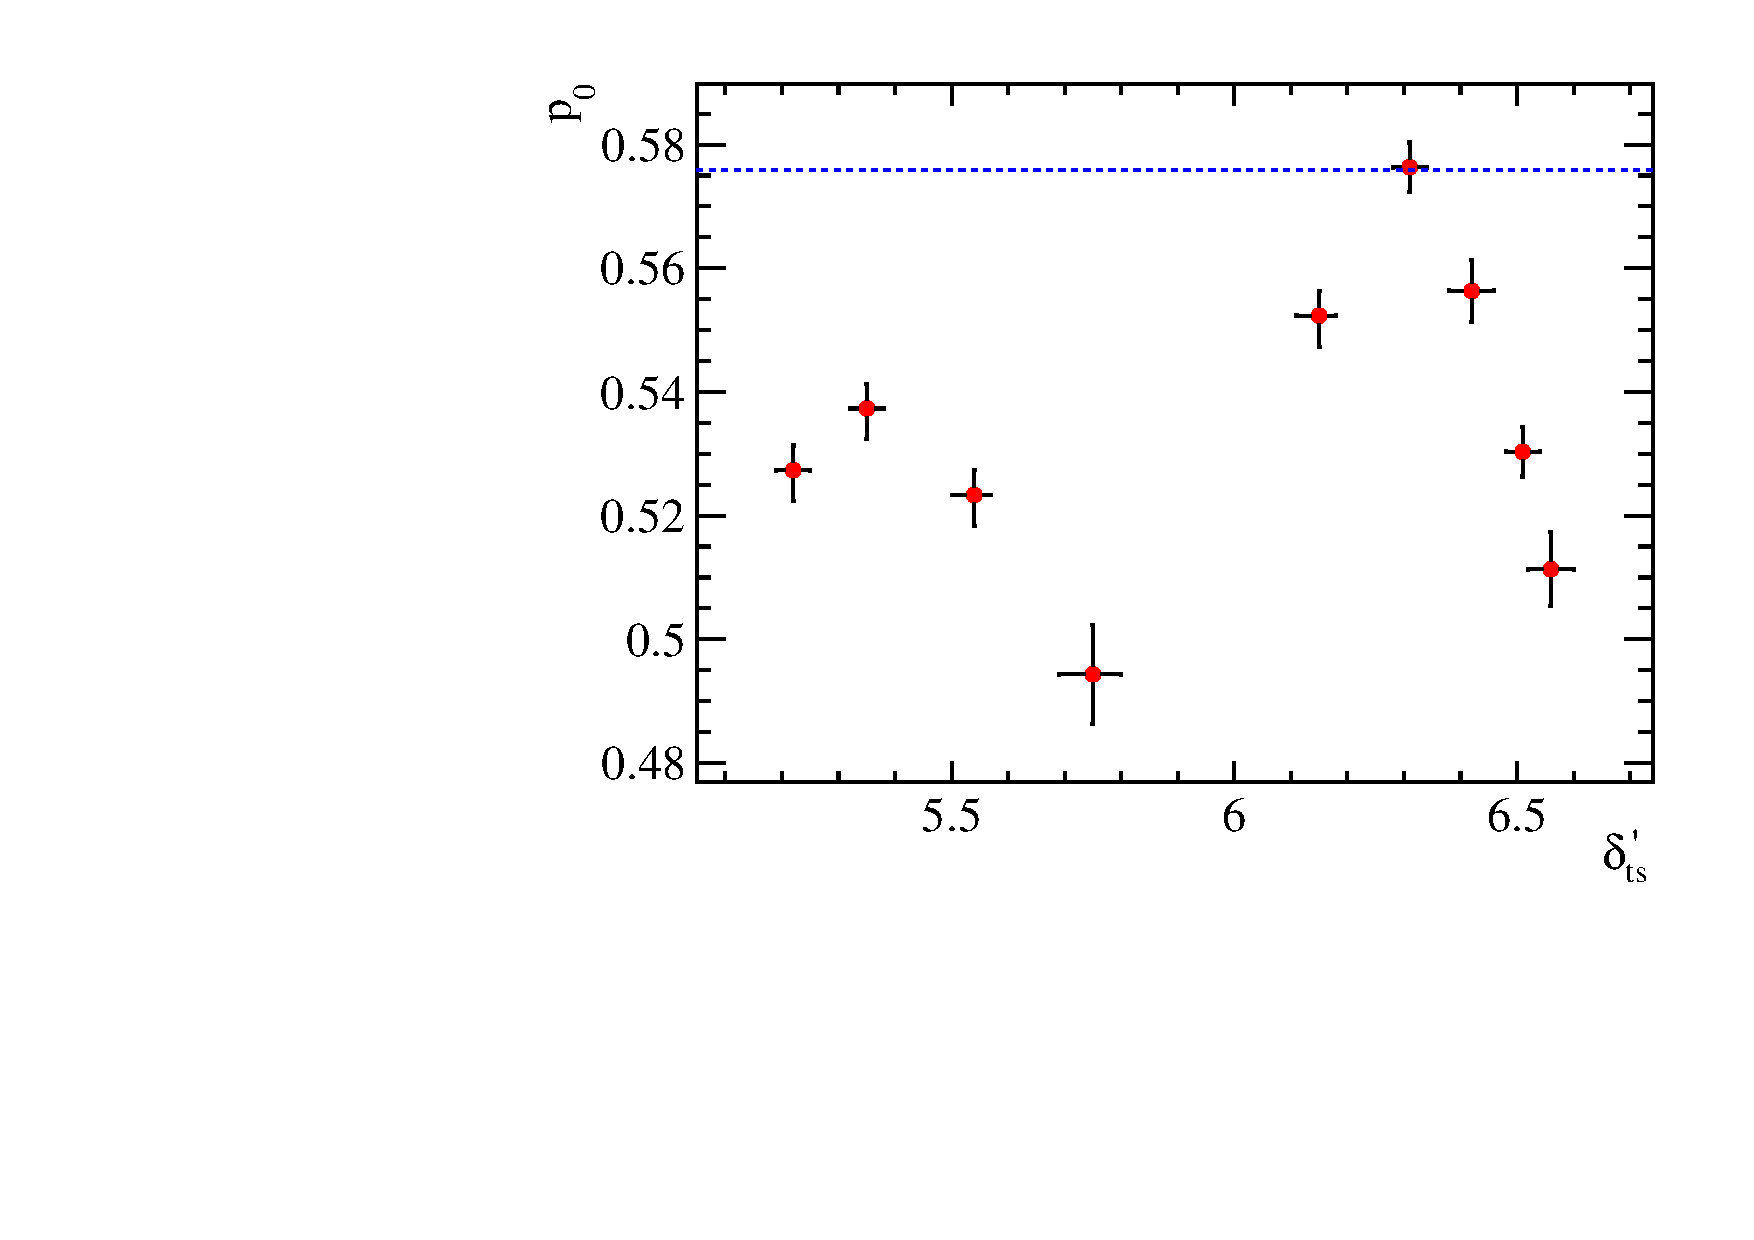
\includegraphics[width=0.9\textwidth]{PMTRelated/GTmodel/true_p.pdf}
	\caption{When performing convolution with 9 MCP-PMTs, the distribution of $\delta_{\mathrm{ts}}'$ and $p_0$ takes place at the point of minimum chi-square. The blue dashed line represents the expected $\hat{p}_0$ that is estimated from~\cite{chen2018photoelectron}. }
	\label{fig:true_p}
\end{figure}

To make a comparison between our measurement and previous studies, we transform \(\delta_\text{ts}'\) into the SEY \(\delta\).
\begin{equation}
	\label{eq:2}
	\delta = \delta_\text{bs} + \delta_\text{rd} + (1-\delta_\text{bs} - \delta_\text{rd}) \delta_\text{ts}'
\end{equation}
and the fraction \(p_0\) to \(p\) is determined by Eq.~\eqref{eq:p0}. Cao et al.~\cite{cao_secondary_2021} measured the secondary electron yield (SEY) of the \ce{Al2O3}-\ce{MgO} double - layered film to be in the range of 4 - 5. Chen et al.~\cite{2016Optimization} noted that there exists an electrostatic lens effect at the entrances of the microchannel plate (MCP) channels. This effect results in the ratio of the PEs entering the MCP channels being smaller than the open - area ratio. When the incident angle of the PEs is \(\theta_0 = 0^\circ\), when the open - area ratio of the MCP is \SI{74.9}{\percent}, the proportion of PEs directly entering the MCP channels is approximately \SI{60}{\percent}. Chen et al.~\cite{chen2018photoelectron} showed that when the open - area ratio is \SI{65}{\percent}, this proportion is around \SI{55}{\percent}. In our study, the MCPs have pore diameters of \SI{12}{\mu\meter}, the spacing between pores is \SI{14} {\mu\meter}, and the open - area ratio is \SI{66.6}{\percent}. For \(\delta_{\mathrm{rd}}+\delta_{\mathrm{bs}} = 0.1\), the expected value of \(\hat{p}_0\) is calculated as \(\hat{p}_0=\frac{55\%}{1-(1 - 55\%)\delta_{\mathrm{rd}}+\delta_{\mathrm{bs}}}\approx 57.6\%\).
\begin{figure}[htbp]
	\centering
	\begin{subfigure}{0.5\textwidth}
		\centering
		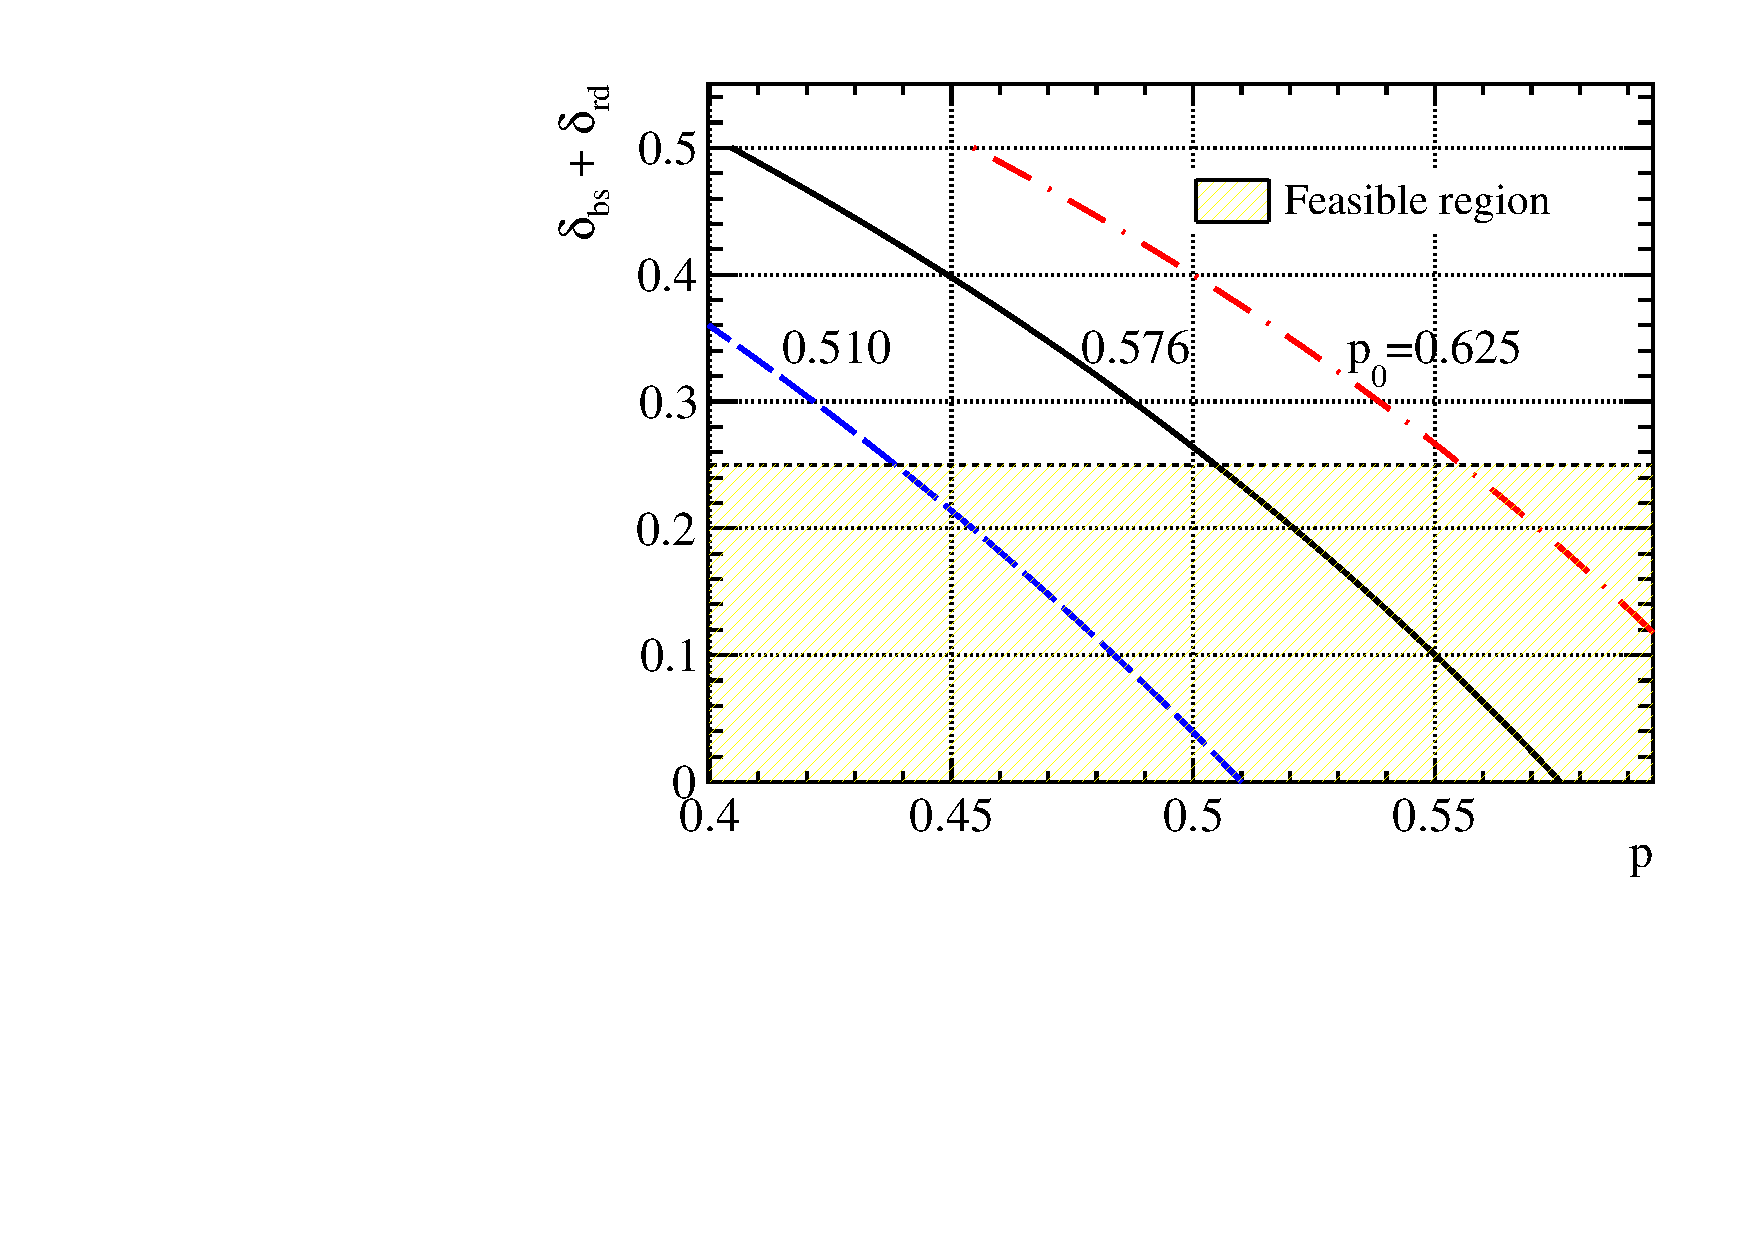
\includegraphics[width=0.9\textwidth]{PMTRelated/GTmodel/parameter_pp0.pdf}
		\caption{}
		\label{fig:pp0}
	\end{subfigure}%
	\hfill
	\begin{subfigure}{0.5\textwidth}
		\centering
		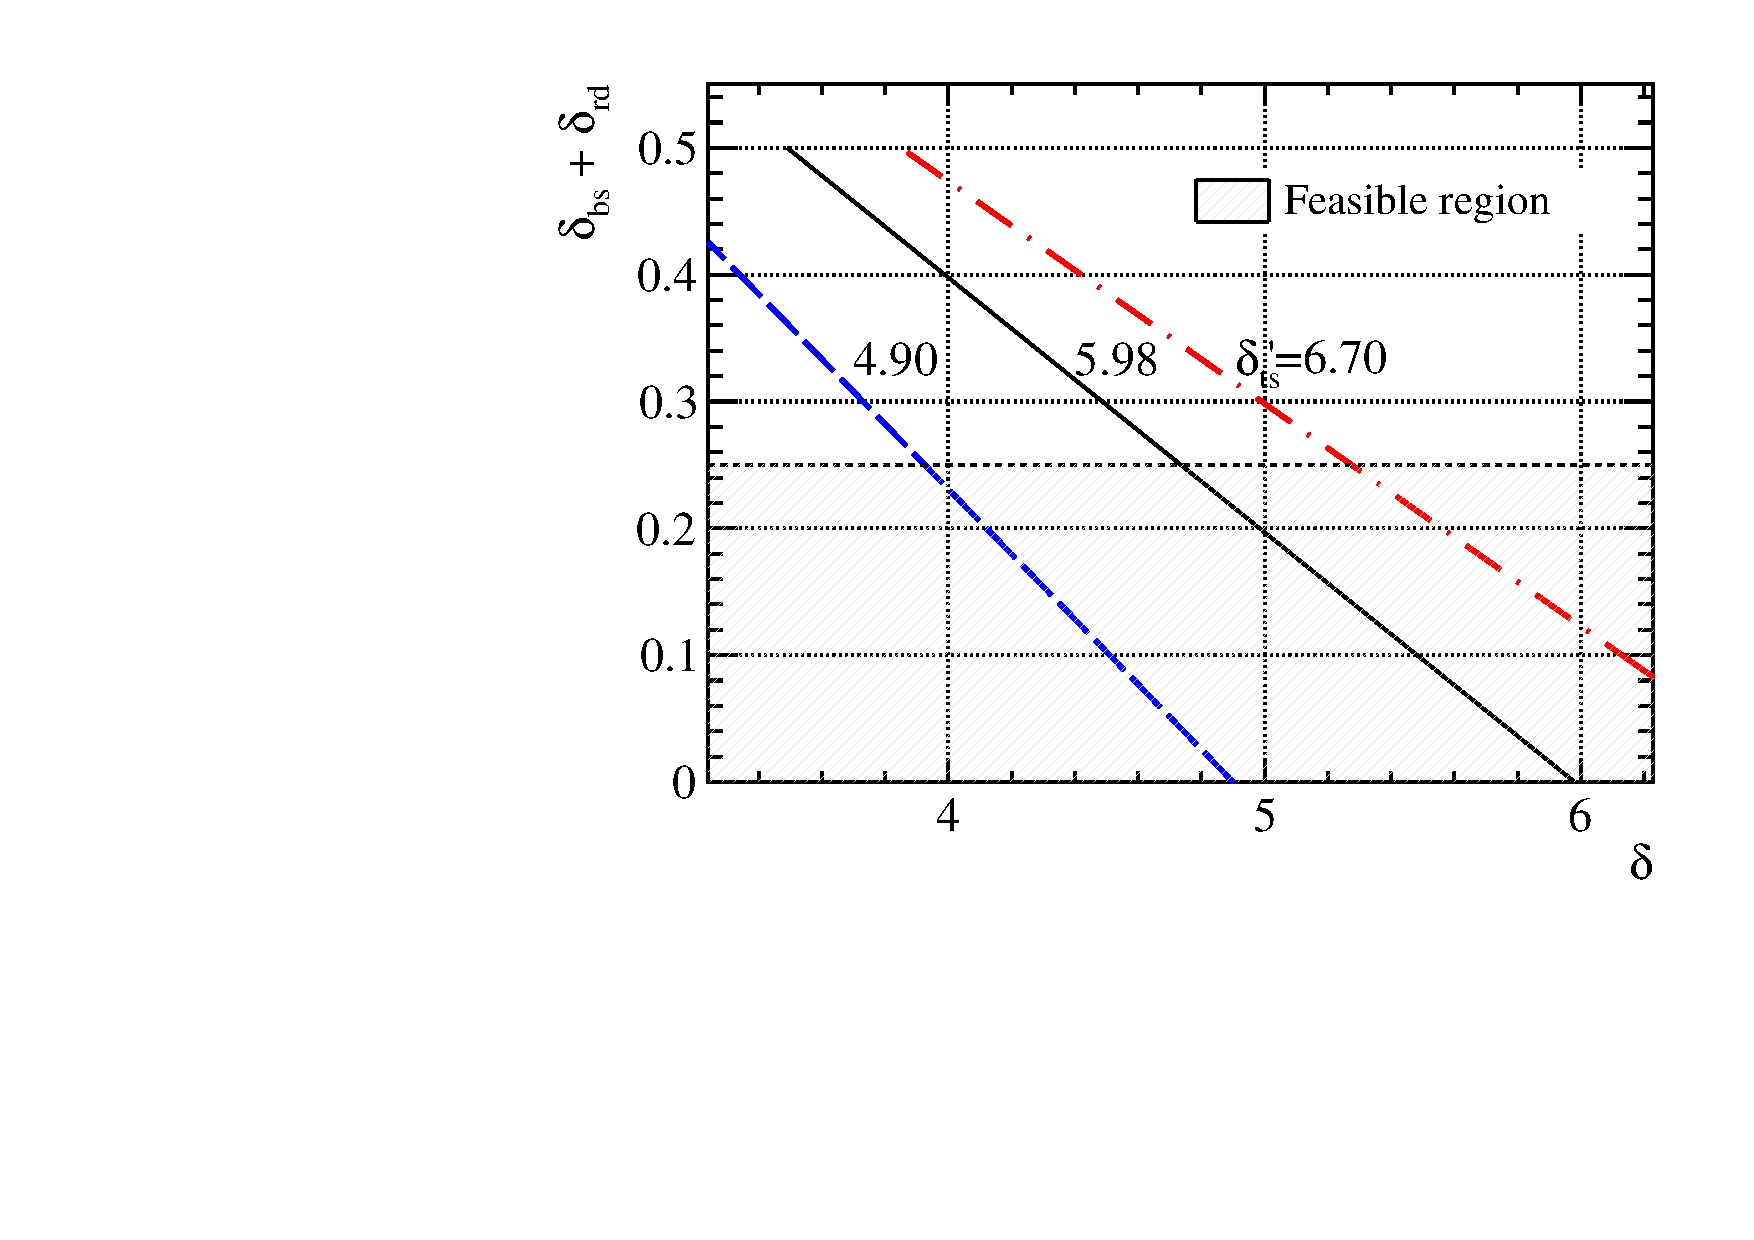
\includegraphics[width=0.9\textwidth]{PMTRelated/GTmodel/parameters_ts.pdf}
		\caption{}
		\label{fig:tsts}
	\end{subfigure}
	\caption{Relations of \(\delta_\text{bs} + \delta_\text{rd}\) vs. the SEY \(\delta\) and the fraction of channel mode \(p\).
		The feasible region shows the consistency of our measurement to the literature.}
	\label{fig:pdelta}
\end{figure}

In Fig.~\ref{fig:pdelta}, when considering the typical values of \(\delta = 5\) and \(p = 0.55\), our measurement aligns with the assumption that \(\delta_\text{bs}+\delta_\text{rd}<0.25\). Beck~\cite{beck_physical_1966} indicated that the minor contribution of back-scattered and rediffused electrons in SEE holds particularly true for insulators featuring a high SEY.


\subsection{Gamma-Tweedie model for MCP-PMT}\label{sec:model}
In our computations, the distribution of the MCP charge response to the true-secondary electrons, denoted as $\varGamma(\alpha_{i},\beta_{i})$, is dictated by their energies $E_{i}$. These energies $E_{i}$ meet the condition $\sum_{i}^{n}E_{i}<E_0$. The incident energy \(E_0\) of the PEs is \SI{650}{eV}, which is over ten times the energies of the true secondaries. Since $n$ adheres to a Poisson distribution with an expected value ranging from 5 to 6.5, the probability that $n$ is greater than 10 is extremely low and can be disregarded. Consequently, the influence of $n$ on $E_{i}$ can be neglected, and the energy \(E_{i}\) has an independent and identical distribution, as illustrated in Fig.~\ref{fig:single_pe}. Correspondingly, the charge response of the MCP to a single true-secondary electron can be treated in the same manner, as presented in Fig.~\ref{fig:single_fit}. Moreover, a single Gamma distribution \(\varGamma(\alpha',\beta')\) is sufficiently adaptable to depict the continuous mixture of \(\int dE_{i}\frac{1} {\delta_{\mathrm{ts}}}\frac{d\delta_{\mathrm{ts}}} {dE_{i}}\varGamma[\alpha(E_{i}),\beta(E_{i})]\).

\begin{figure}[htbp]
	\centering
	\begin{subfigure}{0.5\textwidth}
		\centering
		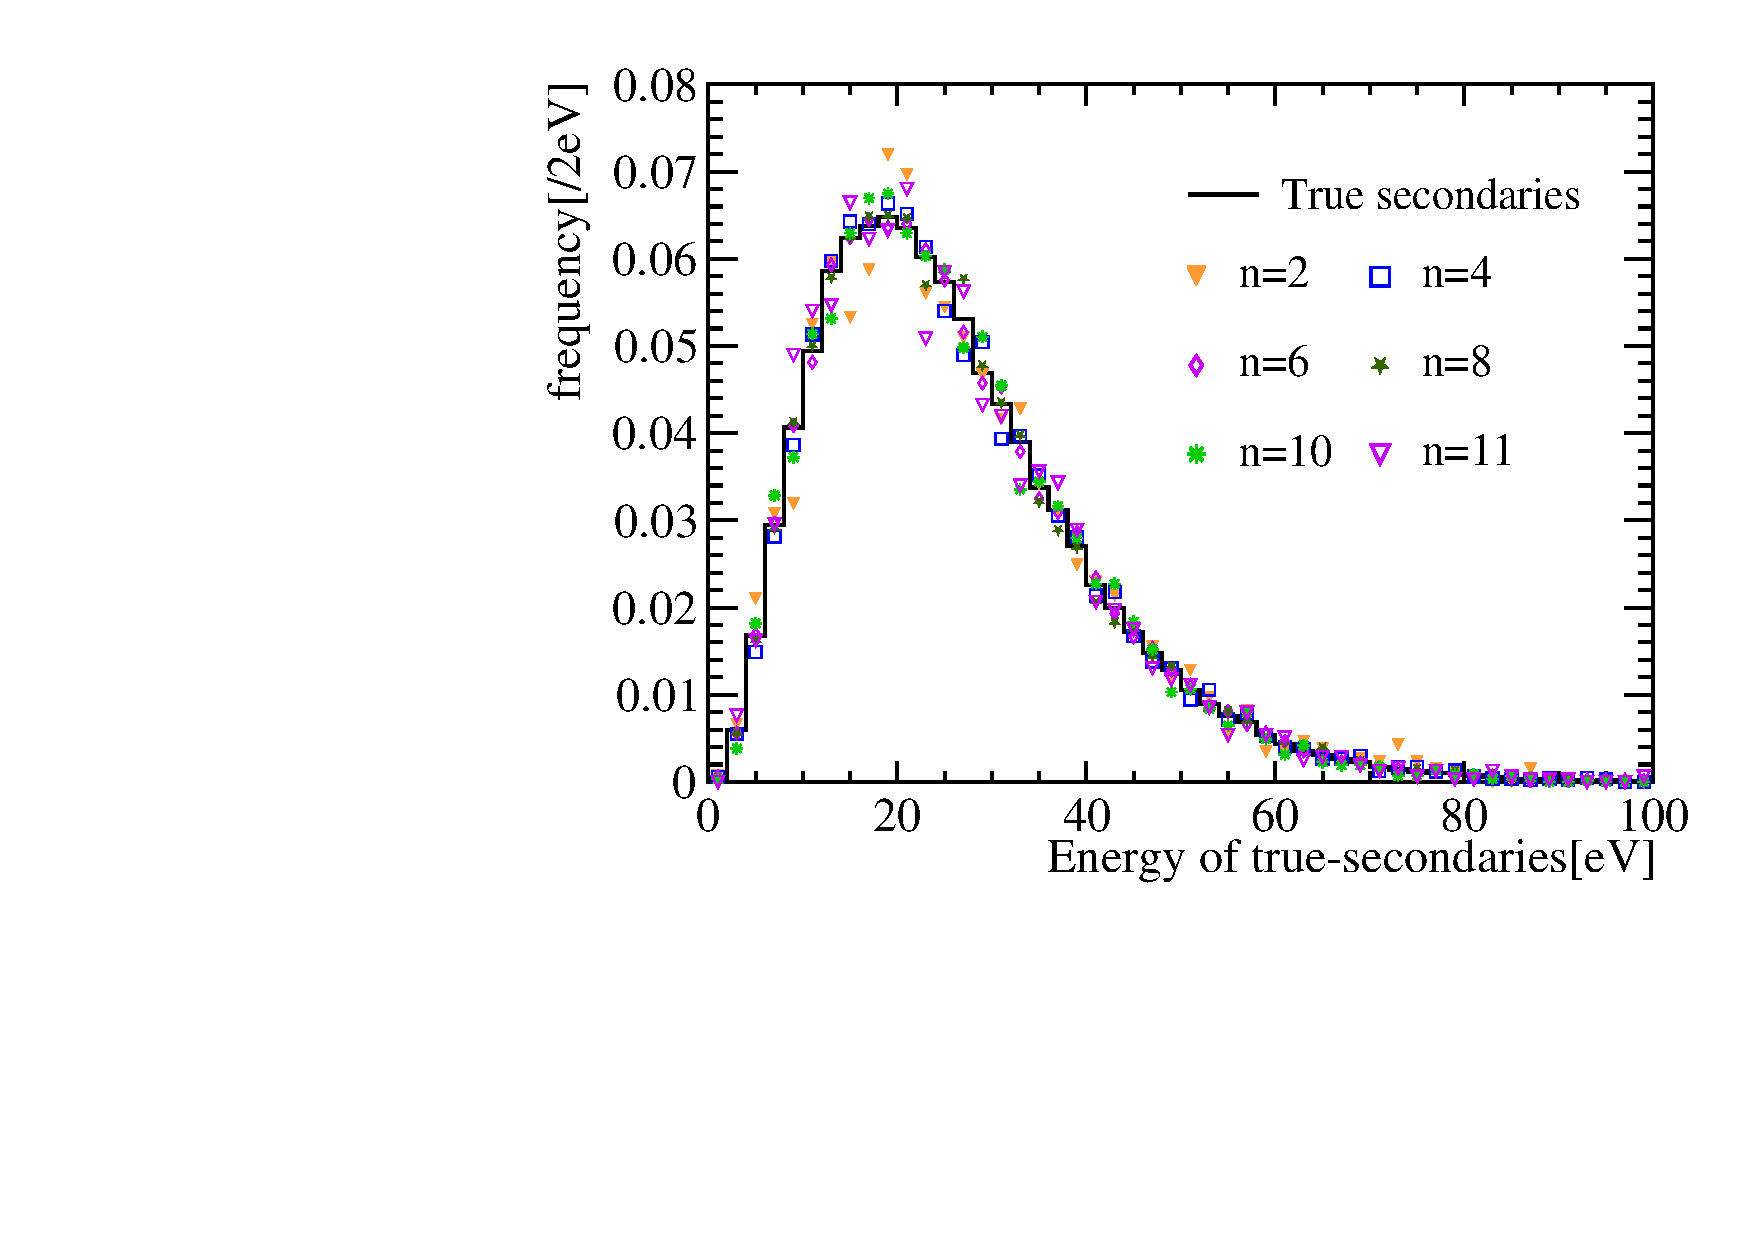
\includegraphics[height=4.5cm]{PMTRelated/GTmodel/single_pecharge.pdf}
		\caption{}
		\label{fig:single_pe}
	\end{subfigure}%
	\hfill
	\begin{subfigure}{0.5\textwidth}
		\centering
		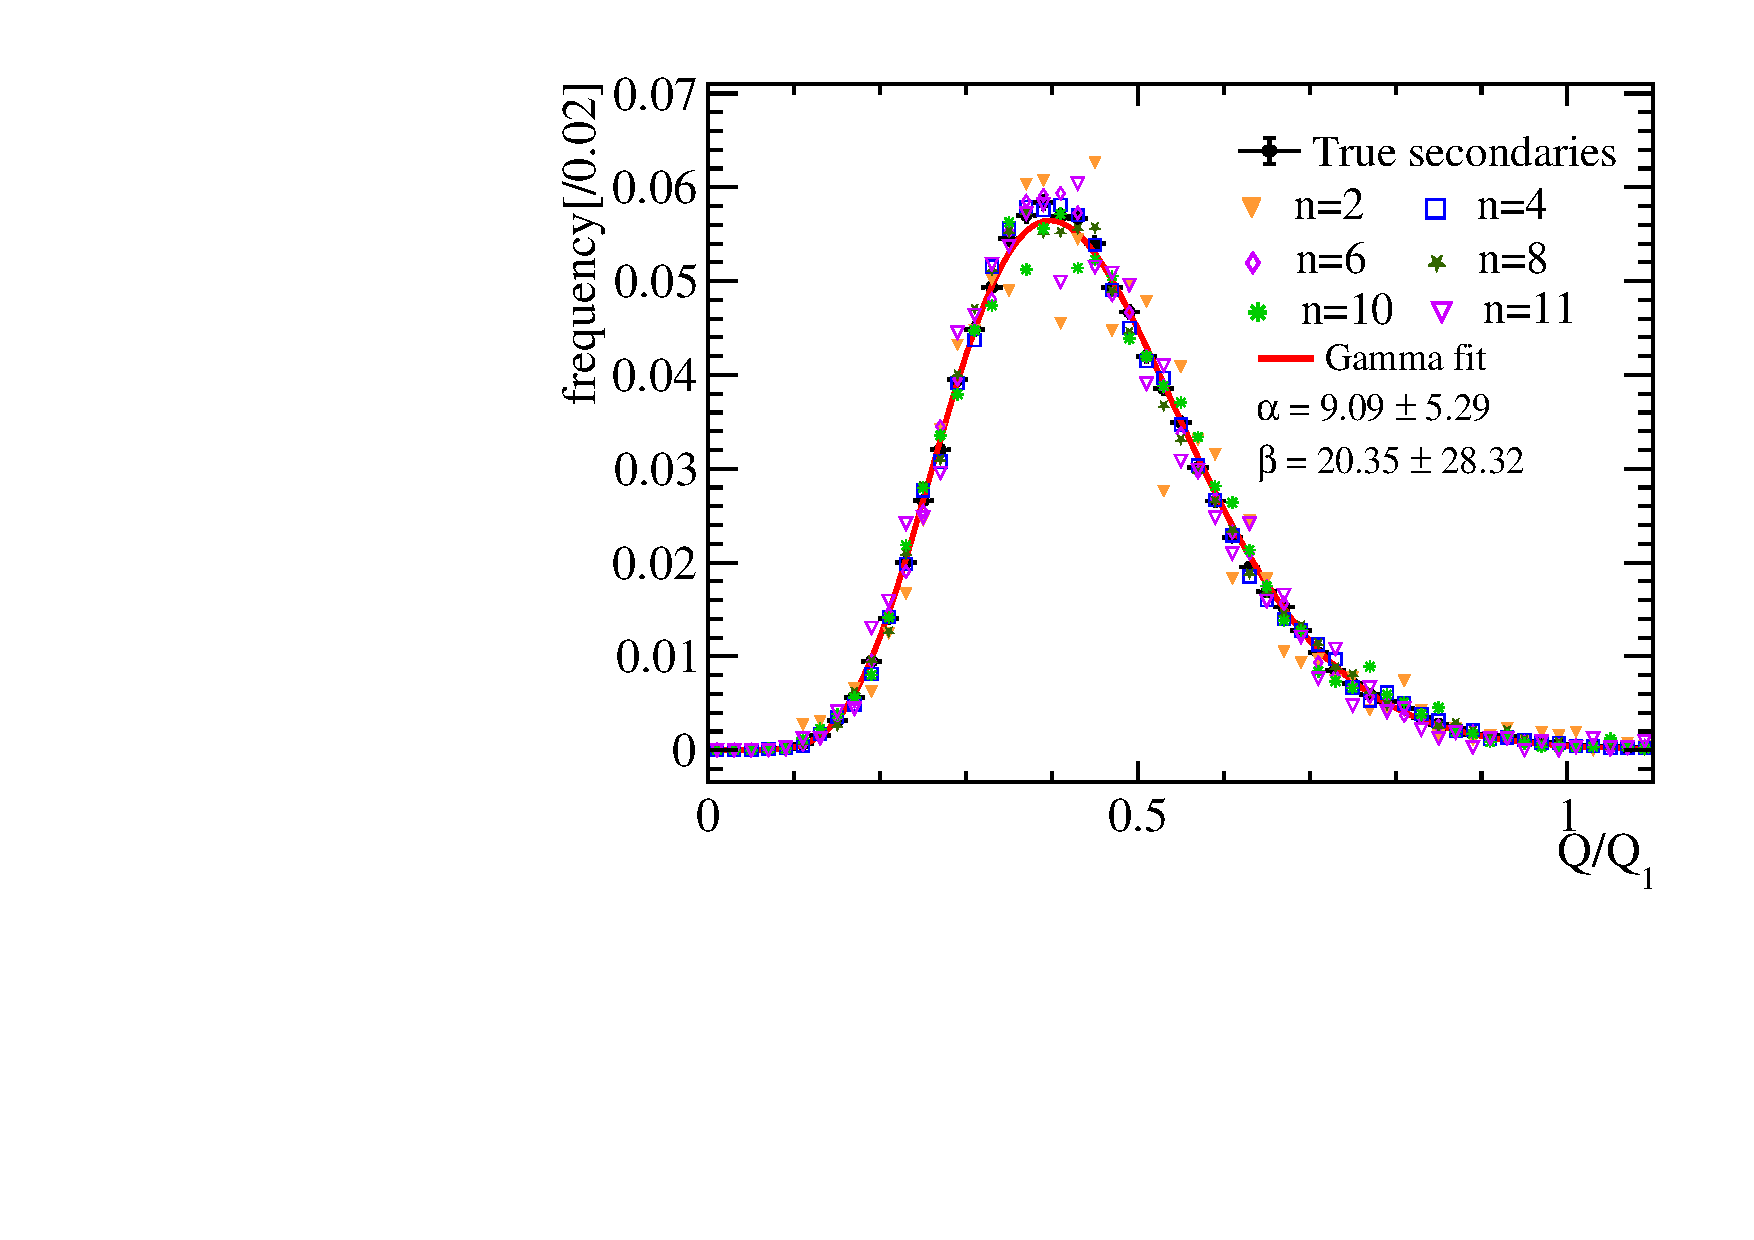
\includegraphics[height=4.65cm]{PMTRelated/GTmodel/singlepefit.pdf}
		\caption{}
		\label{fig:single_fit}
	\end{subfigure}
	\caption{The energy distribution and the charge distribution of MCP to a single true-secondary electron vary with different values of \(n\). \subref{fig:single_pe}: Even when \(n\) takes different values, all the energies of the true secondaries follow the same distribution pattern. \subref{fig:single_fit}: The charge response of MCP to a single true-secondary electron remains the same. Moreover, the fitting with the Gamma distribution \(\varGamma(\alpha',\beta')\) attains an adequate level of goodness. }
	\label{fig:singlepe}
\end{figure}

When we employ such a single \(\varGamma(\alpha', \beta')\) in Equation \eqref{eq:ts_all}, the resulting Poisson-Gamma compound represents a particular instance of the Tweedie distribution $\mathrm{Tw}_{\xi}(\alpha,\beta)$ with \(1 < \xi < 2\) as stated in \cite{1991Tweedie}.
\begin{equation}
	\arraycolsep=1.4pt
	\label{eq:ts_gamma}
	\left.\begin{array}{rl}
		Q_{\text{ts}} & = \sum_{{i}=1}^{n} Q_{i}                 \\
		n             & \sim \mathrm{\pi}(\delta_{\mathrm{ts}}') \\
		Q_{i}         & \sim \varGamma(\alpha', \beta')
	\end{array}\right\} \implies
	Q_{\text{ts}} \sim \mathrm{Tw}_{\xi}(\alpha',\beta')
\end{equation}
A phenomenological joint fit of the \(f_\mathrm{ch}\) Gamma and \(f_\mathrm{ts}\) Tweedie mixture, using Eq.~\eqref{eq:1} and \eqref{eq:ts_gamma}, is adequate for calibrating the SER charge spectrum and measuring \(p_0\) and \(\delta_\text{ts}'\). The relations \(\mu(E_i)\)/\(\sigma(E_i)\) from the voltage division experiment (Sec.~\ref{sec:gain}) and the Furman model help us understand the jumbo charges and justify the phenomenological Gamma - Tweedie mixture. However, they are less useful in practical PMT calibrations.
The number of parameters, two for \(f_\mathrm{ch}\) Gamma and three for \(f_\mathrm{ts}\) Tweedie, can cause difficulties in achieving convergence. This issue can be addressed by applying physical constraints. Usually, $\frac{\alpha'}{\beta'}\approx 0.45Q_1$ and \(\sqrt{\frac{\alpha'}{\beta'^2}}\approx 0.15Q_1\). When the incident energy \(E_0\) is much larger than \(E_{i}\), it is practical to set bounds for them in the ranges of $[0.3,0.7]Q_1$ and $[0.05,0.3]~Q_1$.
We have also examined the chi-square results in the Gamma-Tweedie fitting, and the obtained $\chi^2/\mathrm{ndf}<10$ indicates a good fit. Under these circumstances, we are able to formulate the mathematical model for the SER of the MCP-PMT:
\begin{equation}
	\label{eq:GTmodel}
	f_{\text{MCP-PMT}}(Q) = p_0 \varGamma(Q; \alpha, \beta) + (1-p_0) \mathrm{Tw}_{\xi}(Q; \alpha', \beta')
\end{equation}

\subsection{The gain distribution of PMTs}
We used the charge spectrum of dark noise for gain calibration. As shown in the Fig.~\ref{fig:gain_100range}, we only utilized the information within the first \SI{100}{ns} of each event to ensure obtaining a clean dark noise signal.
For the Dynode-PMTs in JUNO, we deploy the Gamma distribution~($\Gamma(Q;\alpha,\beta)$) for the gain calculation and Gamma-Tweedie distribution~($p_0\Gamma(Q;\alpha,\beta) + (1-p_0)\mathrm{Tw}_{\xi}(Q;\alpha',\beta')$)for MCP-PMTs.
As shown in Fig.~\ref{fig:pmtfit}, for Dynode-PMT, the Gamma distribution can already depict the properties of the main peak extremely clearly. For MCP-PMT, the Gamma-Tweedie distribution can not only clearly describe the long-tail structure, but also demonstrates excellent performance during the fitting process.
In addition to defining the gain of the main peak~($G_p$), we also need to define the average gain~($G_m$) that describes the mean of the entire SER for MCP-PMTs. Therefore, in our work, we have defined the gain of each of the two distributions respectively.
\begin{itemize}
	\item For Dynode-PMTs, $G_m=G_p=\frac{\alpha}{\beta}$
	\item For MCP-PMTs, $G_p=\frac{\alpha}{\beta}$ and $G_m=p_0\frac{\alpha}{\beta}+\lambda\frac{\alpha'}{\beta'}$
\end{itemize}

\begin{figure}[htbp]
	\centering
	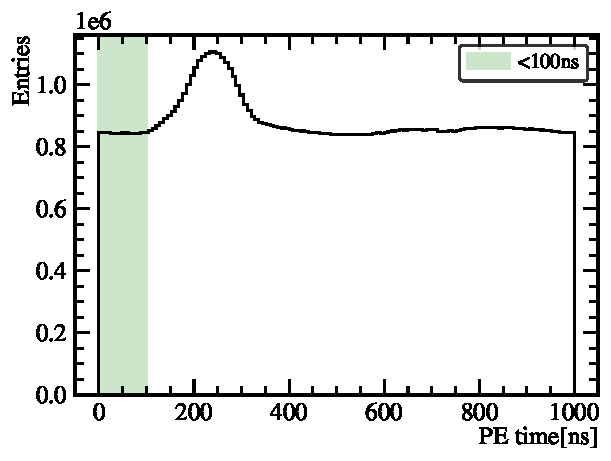
\includegraphics[width=0.5\textwidth]{PMTRelated/Gain_DCR_window.pdf}
	\caption{The range of PE time for gain and calibration. Only the PEs in the first \SI{100}{ns} are used.}
	\label{fig:gain_100range}
\end{figure}

\begin{figure}[htbp]
	\centering
	\begin{subfigure}{0.5\textwidth}
		\centering
		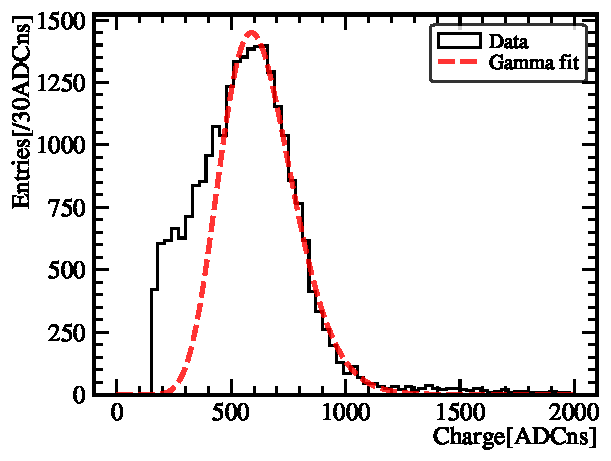
\includegraphics[width=0.9\textwidth]{PMTRelated/Dynode-PMT_fit.pdf}
		\caption{}
		\label{fig:dynode-fit}
	\end{subfigure}%
	\hfill
	\begin{subfigure}{0.5\textwidth}
		\centering
		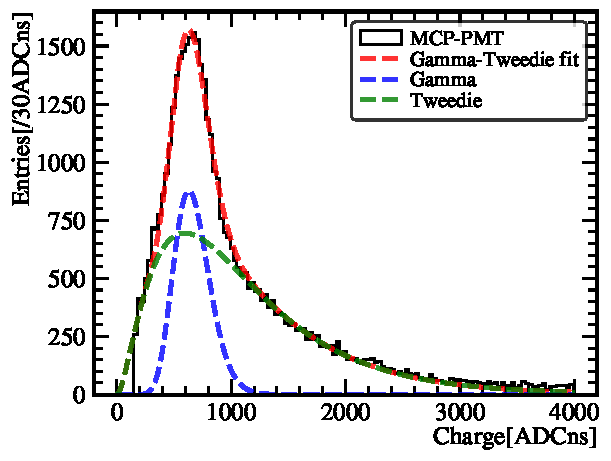
\includegraphics[width=0.9\textwidth]{PMTRelated/MCP-PMT_fit.pdf}
		\caption{}
		\label{fig:mcp-fit}
	\end{subfigure}
	\caption{The gain fit of PMTs. \subref{fig:dynode-fit} shows the Gamma distribution fit of Dynode-PMTs, and \subref{fig:mcp-fit} shows the Gamma-Tweedie fit of MCP-PMTs.}
	\label{fig:pmtfit}
\end{figure}

As illustrated in Fig.~\ref{fig:gmp}, for the two types of PMTs, the fitted $G_p$ values are already aligned quite well. However, regarding $G_m$, the value of MCP-PMT is significantly higher than that of Dynode-PMT. Also, the average gain of MCP-PMTs is much larger than the peak gain. This indicates that in the long-tail structure, $\lambda\frac{\alpha'}{\beta'}$ is greater than $\frac{\alpha}{\beta}$, which is consistent with our experimental conclusion.

\begin{figure}[htbp]
	\centering
	\begin{subfigure}{0.5\textwidth}
		\centering
		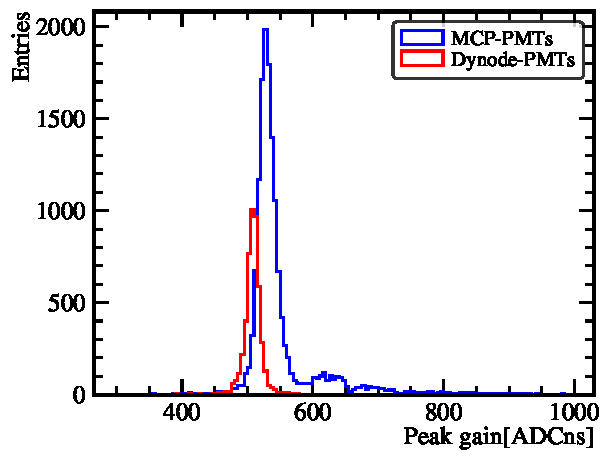
\includegraphics[width=0.9\textwidth]{PMTRelated/gp.pdf}
		\caption{}
		\label{fig:gp}
	\end{subfigure}%
	\hfill
	\begin{subfigure}{0.5\textwidth}
		\centering
		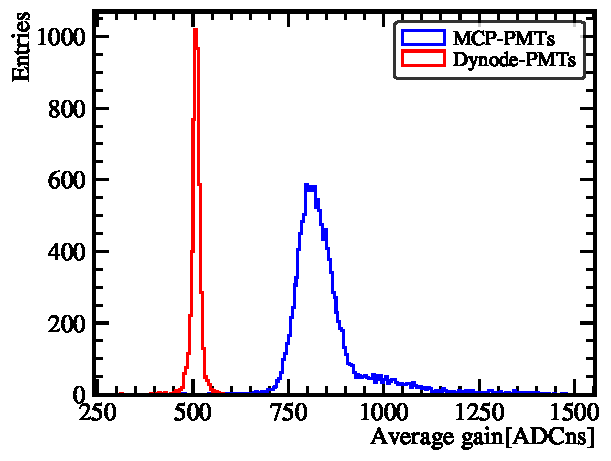
\includegraphics[width=0.9\textwidth]{PMTRelated/gm.pdf}
		\caption{}
		\label{fig:gm}
	\end{subfigure}%
	\hfill
	\begin{subfigure}{0.5\textwidth}
		\centering
		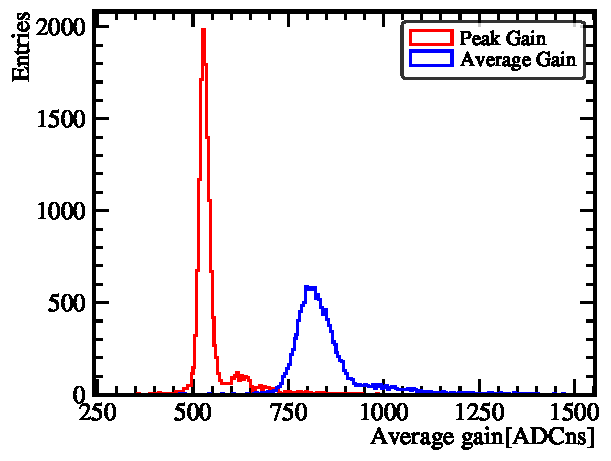
\includegraphics[width=0.9\textwidth]{PMTRelated/mcp-gpm.pdf}
		\caption{}
		\label{fig:gmp_mcp}
	\end{subfigure}
	\caption{The gain distribution of PMTs. \subref{fig:gp} shows the peak gain distribution, \subref{fig:gm} indicated the average gain distribution, and \subref{fig:gmp_mcp} illustrates the peak gain and average gain of MCP-PMTs.}
	\label{fig:gmp}
\end{figure}

\section{The dark count rate}
\label{sec:dcr}
Since we imposed restrictions on the selection of dark noise when performing gain calibration, on this basis, the dark noise count rate~(DCR) of the PMT can be calibrated. The formula used to calculate the DCR is Eq.~\eqref{eq:dcr}. $n_{PE,100}$ is the number of PEs in first \SI{100}{ns} and $n_w$ is the number of events.
\begin{equation}
	DCR=\frac{n_{PE,100}}{n_w*100}
	\label{eq:dcr}
\end{equation}
Taking Run~3279 on February 2nd as an example, the distribution of the DCR obtained from the calibration is shown in the Fig.~\ref{fig:dcr_calib}. It can be seen that the mean dark noise rate of the MCP-PMT is about \SI{33}{kHz}, which is about \SI{5}{kHz} higher than that of the Dynode-PMT. At the same time, from the perspective of the position distribution, the distribution of the DCR is relatively uniform and there is no obvious asymmetry.
\begin{figure}[htbp]
	\centering
	\begin{subfigure}{0.6\textwidth}
		\centering
		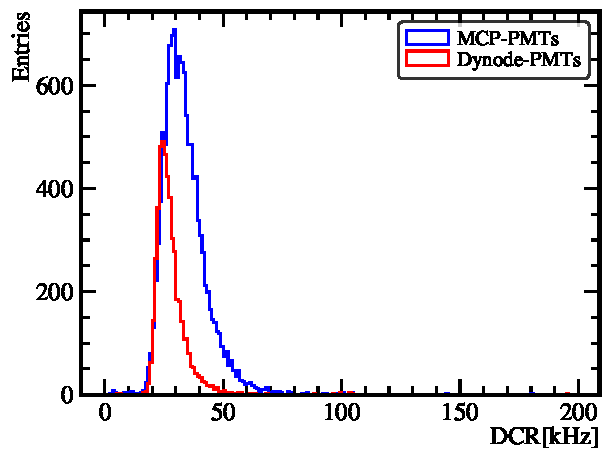
\includegraphics[width=\textwidth]{PMTRelated/dcr_3279.pdf}
		\caption{}
		\label{fig:dcr}
	\end{subfigure}%
	\hfill
	\begin{subfigure}{\textwidth}
		\centering
		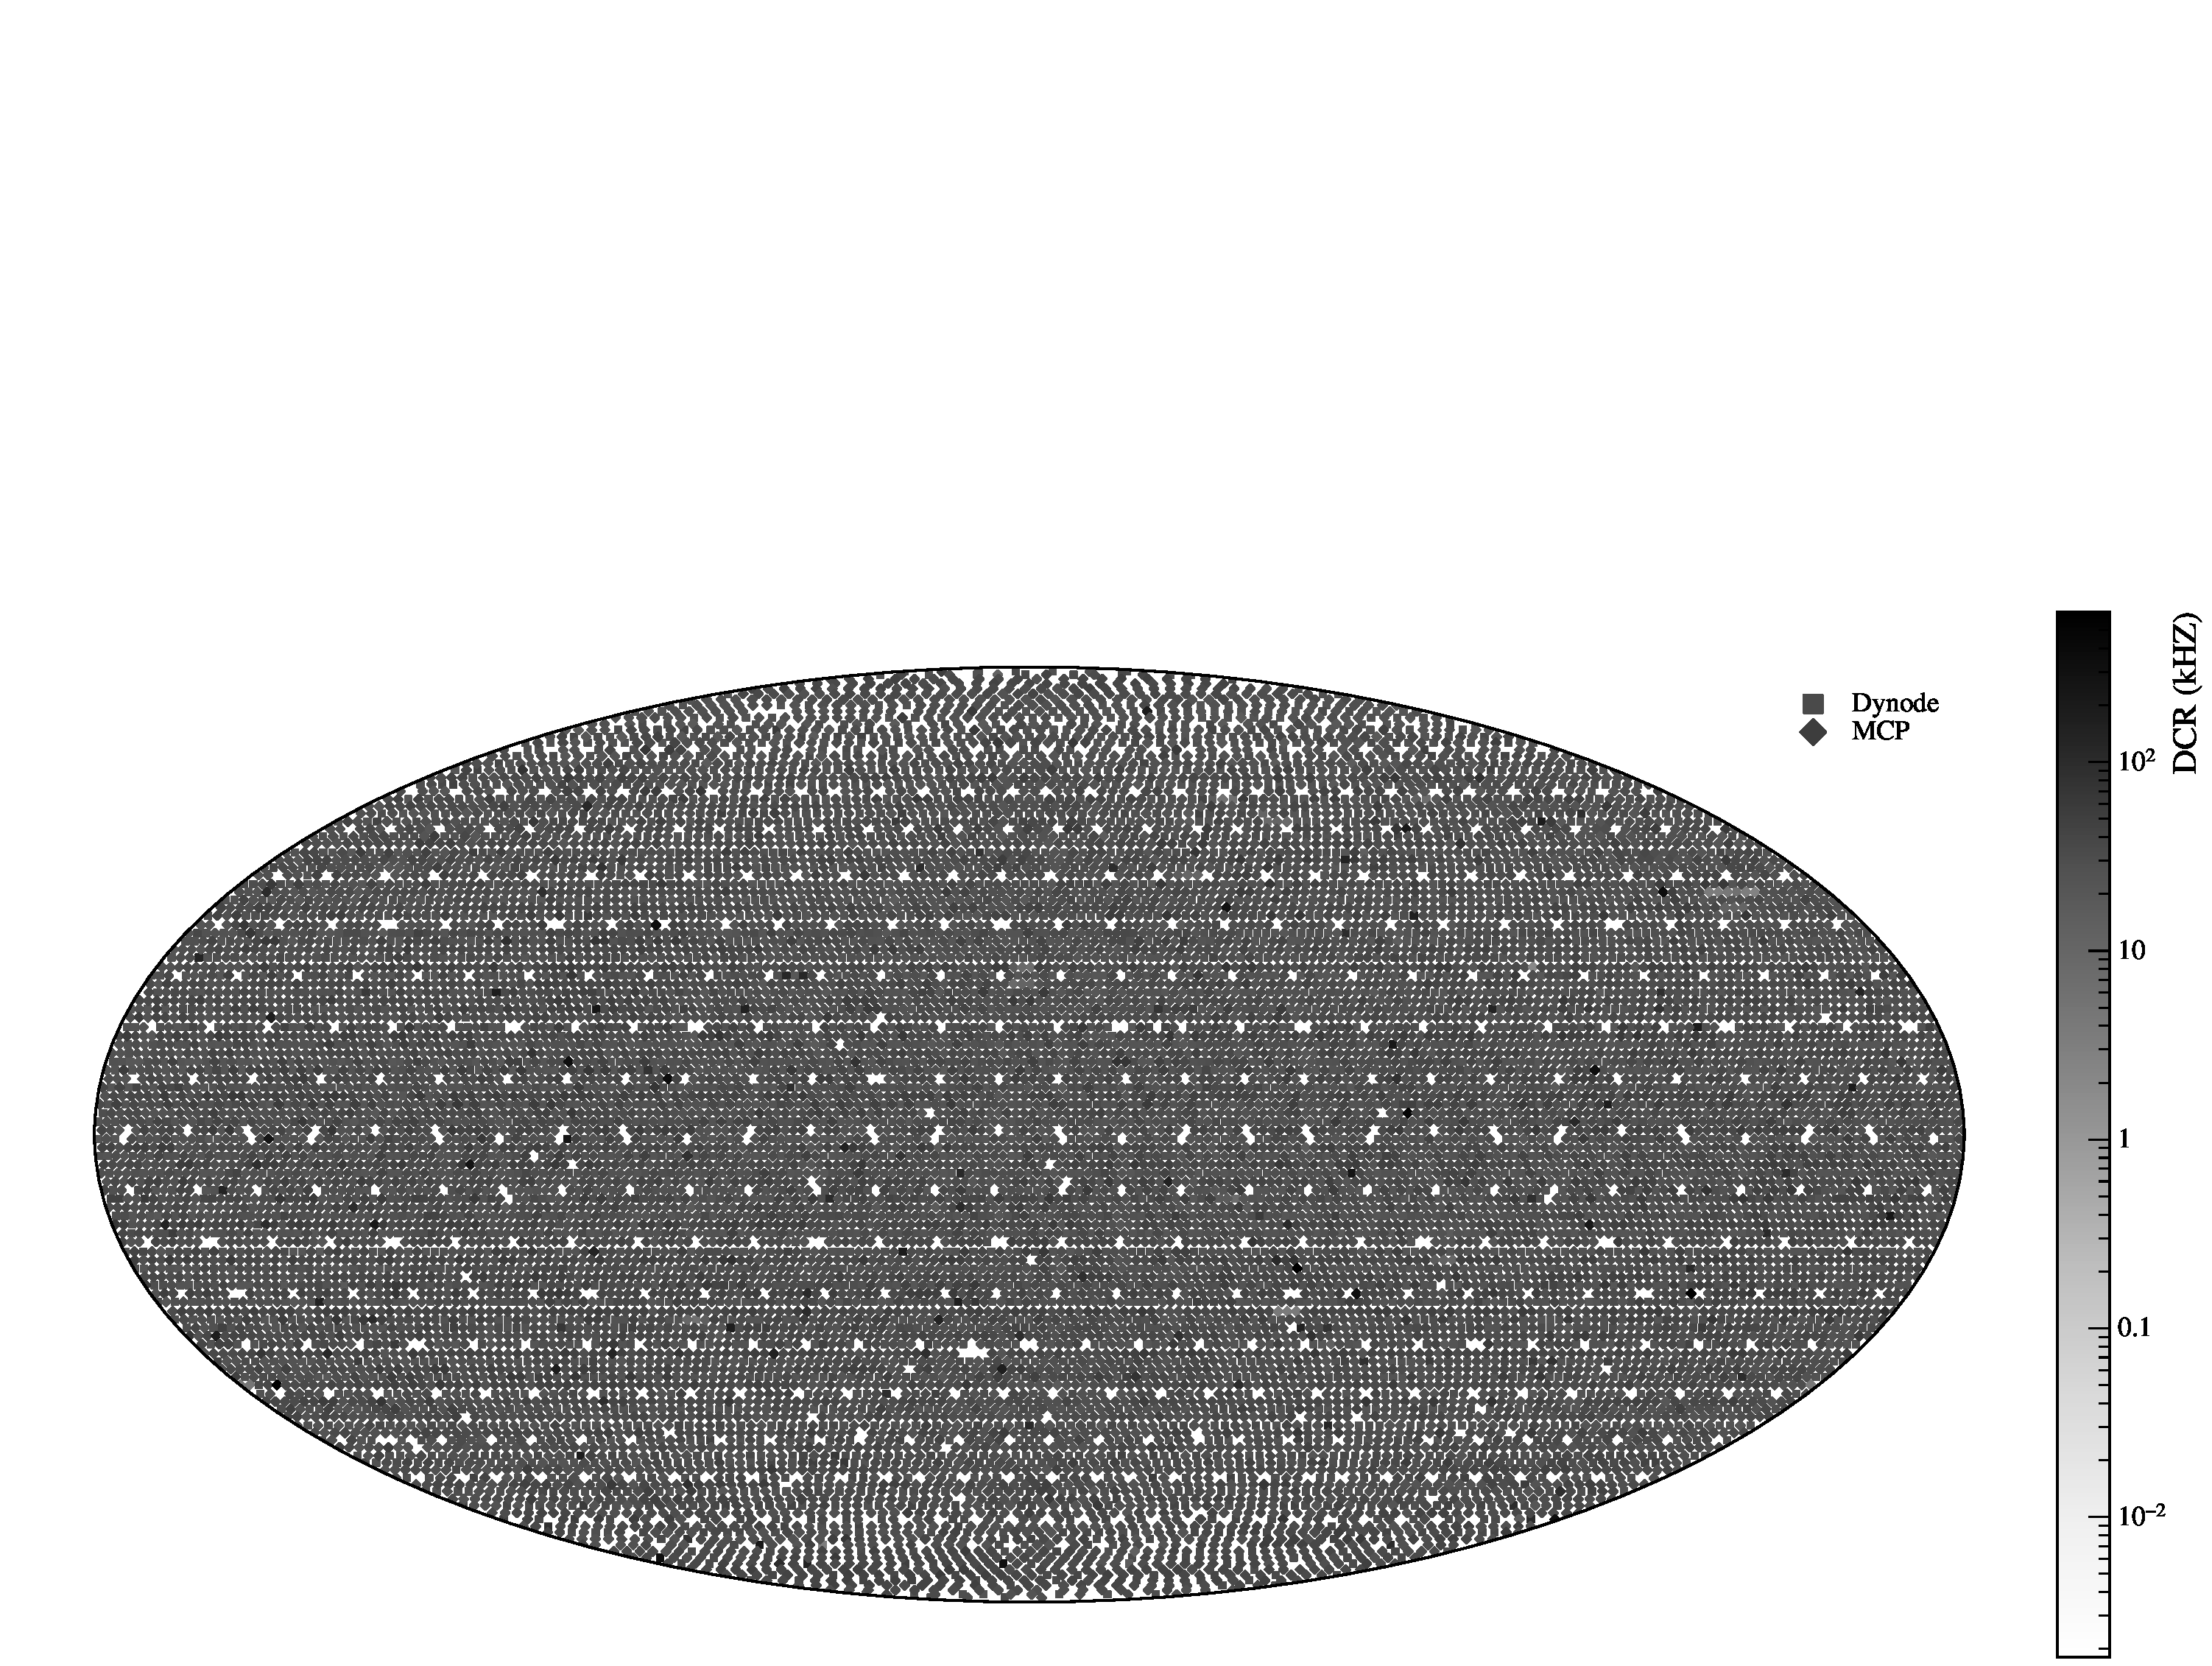
\includegraphics[width=\textwidth]{PMTRelated/dcr_3279_pos.pdf}
		\caption{}
		\label{fig:dcrpos}
	\end{subfigure}
	\caption{The DCR distribution of PMTs. In \subref{fig:dcr}, the blue line shows the DCR of MCP-PMTs and the red one shows that of Dynode-PMTs. \subref{fig:dcrpos} shows the postion distribution of DCR.}
	\label{fig:dcr_calib}
\end{figure}
For each analyzed run, the DCR was calibrated independently. Consequently, the variation law of DCR with the data acquisition time can be straightforwardly investigated, as shown in Fig.~\ref{fig:dcr_time}. It has been observed that as the detector is in operation, the DCR initially increased, then gradually decreased, and ultimately stabilized. Throughout this transformation process, the DCR of the MCP-PMT consistently remained approximately \SI{5}{kHz} higher than that of the Dynode-PMT. Simultaneously, the DCRs of both PMTs consistently exceeded \SI{20}{kHz}. This situation exerted a certain influence on and presents challenges to the Cherenkov reconstruction of the water phase. Thus, it was essential to develop a mathematical model of the dark noise and apply it to the reconstruction.
\begin{figure}[htbp]
	\centering
	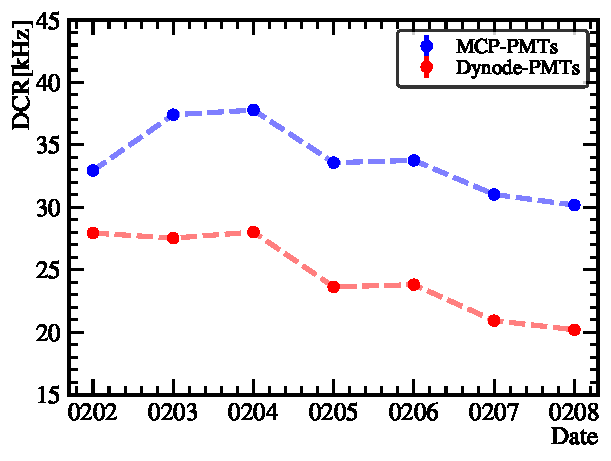
\includegraphics[width=0.5\textwidth]{PMTRelated/dcr_time.pdf}
	\caption{The curve of DCR changing with time.}
	\label{fig:dcr_time}
\end{figure}

\section{The timing calibration}
\label{sec:tts}
In the water phase, the time characteristics are calibrated by laser.
What has a relatively large impact on the subsequent reconstruction are the time starting point of each PMT, that is, the time-offset, and the transit time spread~(TTS) of the PMT. In this work, we use the standard deviation to represent TTS instead of using the full width at half maximum.
The distribution of time-offset is as shown in Fig.~\ref{fig:offset} and that of TTS is as illustrated in Fig.~\ref{fig:tts}. The timing jitter (TTS) of the MCP-PMT is around \SI{10}{ns}, which is significantly higher than that of the Dynode-PMT (around \SI{2.5}{ns}). Therefore, in the reconstruction, the impact of TTS cannot be ignored, and modeling and application are required.
\begin{figure}[htbp]
	\centering
	\begin{subfigure}{0.5\textwidth}
		\centering
		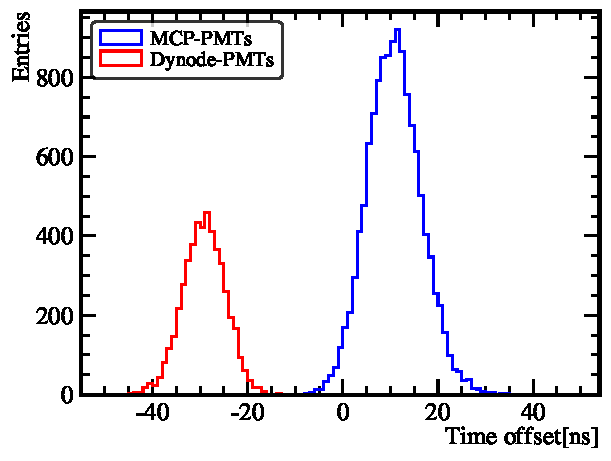
\includegraphics[width=0.9\textwidth]{PMTRelated/offset.pdf}
		\caption{}
		\label{fig:offset}
	\end{subfigure}%
	\hfill
	\begin{subfigure}{0.5\textwidth}
		\centering
		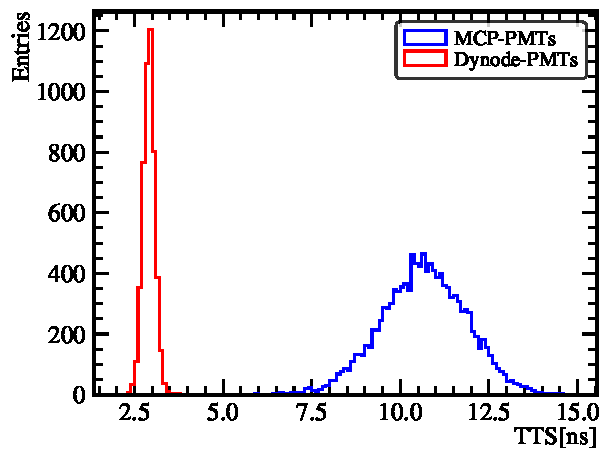
\includegraphics[width=0.9\textwidth]{PMTRelated/TTS.pdf}
		\caption{}
		\label{fig:tts}
	\end{subfigure}
	\caption{The timing characteristics in water phase. \subref{fig:offset} shows the distribution of time-offset and \subref{fig:tts} illustrates the distribution of TTS.}
	\label{fig:timeCailb}
\end{figure}

\section{The Photon Detection Efficiency}
The Photon Detection Efficiency~(PDE, $\varepsilon$) is an important parameter for measuring the photon detection ability of a PMT. Numerically, it is equal to the product of QE and CE. In this work, we directly use the results obtained from the batch tests at Pan-Asia~\cite{JUNO:2022hlz}, as shown in Fig.~\ref{fig:PDE}.
\begin{figure}[htbp]
	\centering
	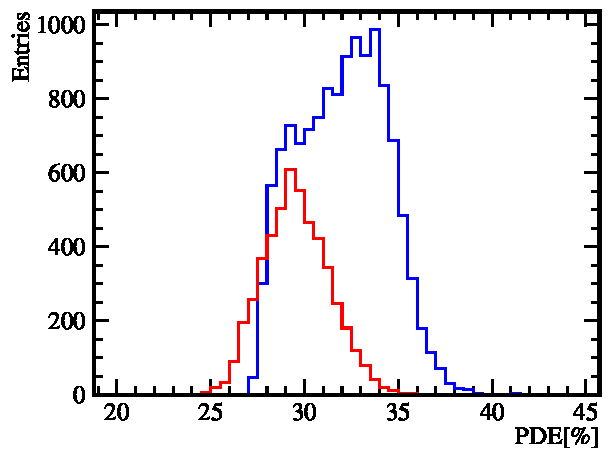
\includegraphics[width=0.5\textwidth]{PMTRelated/PDE.pdf}
	\caption{The distribution of PDE.}
	\label{fig:PDE}
\end{figure}